\documentclass{article}
\usepackage{amsmath}
\usepackage{color,pxfonts,fix-cm}
\usepackage{latexsym}
\usepackage[mathletters]{ucs}
\DeclareUnicodeCharacter{8211}{\textendash}
\DeclareUnicodeCharacter{34}{\textquotedbl}
\DeclareUnicodeCharacter{8220}{\textquotedblleft}
\DeclareUnicodeCharacter{46}{\textperiodcentered}
\DeclareUnicodeCharacter{8221}{\textquotedblright}
\DeclareUnicodeCharacter{58}{$\colon$}
\DeclareUnicodeCharacter{8226}{$\bullet$}
\DeclareUnicodeCharacter{8217}{\textquoteright}
\DeclareUnicodeCharacter{62}{\textgreater}
\DeclareUnicodeCharacter{32}{$\ $}
\usepackage[T1]{fontenc}
\usepackage[utf8x]{inputenc}
\usepackage{pict2e}
\usepackage{wasysym}
\usepackage[english]{babel}
\usepackage{tikz}
\pagestyle{empty}
\usepackage[margin=0in,paperwidth=595pt,paperheight=842pt]{geometry}
\begin{document}
\definecolor{color_29791}{rgb}{0,0,0}
\definecolor{color_157489}{rgb}{0.513726,0.227451,0.035294}
\definecolor{color_139071}{rgb}{0.439216,0.188235,0.627451}
\definecolor{color_214303}{rgb}{0.752941,0,0}
\definecolor{color_35327}{rgb}{0,0.690196,0.313726}
\definecolor{color_155902}{rgb}{0.498039,0.498039,0.498039}
\definecolor{color_245272}{rgb}{0.85098,0.85098,0.85098}
\definecolor{color_37858}{rgb}{0.019608,0.388235,0.756863}
\begin{tikzpicture}[overlay]\path(0pt,0pt);\end{tikzpicture}
\begin{picture}(-5,0)(2.5,0)
\put(519.48,-97.53003){\fontsize{11}{1}\usefont{T1}{cmr}{m}{n}\selectfont\color{color_29791}  }
\put(39.025,-783.975){\fontsize{14}{1}\usefont{T1}{cmr}{m}{n}\selectfont\color{color_29791} }
\put(48.65,-84.95){
\includegraphics[width=467.55pt,height=52.45pt]{latexImage_7044ae2d5aa88d56d597a9257795eea2.png}}
\put(286.13,-114.28){\fontsize{28}{1}\usefont{T1}{cmr}{b}{n}\selectfont\color{color_157489}  }
\put(274.63,-145.3){\fontsize{24}{1}\usefont{T1}{cmr}{b}{n}\selectfont\color{color_157489}A  }
\put(190.85,-176.3){\fontsize{20}{1}\usefont{T1}{cmr}{b}{n}\selectfont\color{color_157489}Micro Project Report  }
\put(271.88,-201.55){\fontsize{16}{1}\usefont{T1}{cmr}{b}{n}\selectfont\color{color_29791}On  }
\put(75.3,-238.83){\fontsize{20}{1}\usefont{T1}{cmr}{b}{n}\selectfont\color{color_139071}“CREDIT CARD FRAUD DETECTION USING      }
\end{picture}
\begin{tikzpicture}[overlay]
\path(0pt,0pt);
\filldraw[color_139071][even odd rule]
(85.3pt, -243.08pt) -- (493.97pt, -243.08pt)
 -- (493.97pt, -243.08pt)
 -- (493.97pt, -241.08pt)
 -- (493.97pt, -241.08pt)
 -- (85.3pt, -241.08pt) -- cycle
;
\end{tikzpicture}
\begin{picture}(-5,0)(2.5,0)
\put(156.58,-262.83){\fontsize{20}{1}\usefont{T1}{cmr}{b}{n}\selectfont\color{color_139071}LOGISTICS REGRESSION” }
\end{picture}
\begin{tikzpicture}[overlay]
\path(0pt,0pt);
\filldraw[color_139071][even odd rule]
(156.58pt, -267.08pt) -- (402.93pt, -267.08pt)
 -- (402.93pt, -267.08pt)
 -- (402.93pt, -265.08pt)
 -- (402.93pt, -265.08pt)
 -- (156.58pt, -265.08pt) -- cycle
;
\end{tikzpicture}
\begin{picture}(-5,0)(2.5,0)
\put(164.58,-290.1){\fontsize{16}{1}\usefont{T1}{cmr}{m}{n}\selectfont\color{color_29791}Submitted in partial fulfilment of the  }
\put(141.08,-318.85){\fontsize{16}{1}\usefont{T1}{cmr}{m}{n}\selectfont\color{color_29791}Requirements for the award of the degree of  }
\put(202.85,-347.6){\fontsize{16}{1}\usefont{T1}{cmr}{b}{n}\selectfont\color{color_214303}Bachelor of Technology  }
\put(275.13,-376.12){\fontsize{16}{1}\usefont{T1}{cmr}{b}{n}\selectfont\color{color_29791}In  }
\put(167.83,-404.87){\fontsize{16}{1}\usefont{T1}{cmr}{b}{n}\selectfont\color{color_214303}Computer Science \& Engineering  }
\put(211.6,-433.12){\fontsize{16}{1}\usefont{T1}{cmr}{b}{n}\selectfont\color{color_214303}CYBER SECURITY  }
\put(273.38,-461.65){\fontsize{16}{1}\usefont{T1}{cmr}{b}{n}\selectfont\color{color_29791}By  }
\put(147.83,-490.4){\fontsize{16}{1}\usefont{T1}{cmr}{b}{n}\selectfont\color{color_35327}KVG ARJUN PRASAD     21R21A6264  }
\put(147.83,-519.4){\fontsize{16}{1}\usefont{T1}{cmr}{b}{n}\selectfont\color{color_35327}V.LUKMAN                        21R21A6260  }
\put(150.08,-548.17){\fontsize{16}{1}\usefont{T1}{cmr}{b}{n}\selectfont\color{color_35327}V.BHANU SRI                   21R21A6262  }
\put(149.83,-577.18){\fontsize{16}{1}\usefont{T1}{cmr}{b}{n}\selectfont\color{color_35327}G.SUDEEP                         22R25A6201  }
\put(284.63,-600.92){\fontsize{16}{1}\usefont{T1}{cmr}{b}{n}\selectfont\color{color_29791}  }
\put(211.6,-628.93){\fontsize{16}{1}\usefont{T1}{cmr}{m}{n}\selectfont\color{color_29791}Under the guidance of  }
\put(200.6,-657.95){\fontsize{16}{1}\usefont{T1}{cmr}{b}{n}\selectfont\color{color_29791}Mr. IRFAN BAGAWAN  }
\put(250.63,-686.7){\fontsize{16}{1}\usefont{T1}{cmr}{b}{n}\selectfont\color{color_29791}Professor  }
\put(284.38,-708.7){\fontsize{14}{1}\usefont{T1}{cmr}{b}{n}\selectfont\color{color_29791}  }
\put(116.05,-738.975){\fontsize{16}{1}\usefont{T1}{cmr}{b}{n}\selectfont\color{color_139071}Department of Computer Science \& Engineering  }
\end{picture}
\newpage
\begin{tikzpicture}[overlay]\path(0pt,0pt);\end{tikzpicture}
\begin{picture}(-5,0)(2.5,0)
\put(519.48,-97.53003){\fontsize{11}{1}\usefont{T1}{cmr}{m}{n}\selectfont\color{color_29791}  }
\put(39.025,-783.975){\fontsize{14}{1}\usefont{T1}{cmr}{m}{n}\selectfont\color{color_29791} }
\put(48.65,-84.95){
\includegraphics[width=467.55pt,height=52.45pt]{latexImage_7044ae2d5aa88d56d597a9257795eea2.png}}
\put(211.6,-116.05){\fontsize{16}{1}\usefont{T1}{cmr}{b}{n}\selectfont\color{color_139071}CYBER SECURITY  }
\put(39.025,-144.3){\fontsize{11}{1}\usefont{T1}{cmr}{m}{n}\selectfont\color{color_29791} 2025    }
\put(284.63,-169.55){\fontsize{16}{1}\usefont{T1}{cmr}{b}{n}\selectfont\color{color_139071}  }
\put(115.8,-197.8){\fontsize{16}{1}\usefont{T1}{cmr}{b}{n}\selectfont\color{color_29791}Department of Computer Science \& Engineering  }
\put(211.6,-226.58){\fontsize{16}{1}\usefont{T1}{cmr}{b}{n}\selectfont\color{color_29791}CYBER SECURITY  }
\put(284.63,-250.58){\fontsize{16}{1}\usefont{T1}{cmr}{b}{n}\selectfont\color{color_29791}  }
\put(232.85,-278.58){\fontsize{16}{1}\usefont{T1}{cmr}{b}{n}\selectfont\color{color_29791}CERTIFICATE  }
\end{picture}
\begin{tikzpicture}[overlay]
\path(0pt,0pt);
\filldraw[color_29791][even odd rule]
(232.85pt, -281.83pt) -- (342.4pt, -281.83pt)
 -- (342.4pt, -281.83pt)
 -- (342.4pt, -280.33pt)
 -- (342.4pt, -280.33pt)
 -- (232.85pt, -280.33pt) -- cycle
;
\end{tikzpicture}
\begin{picture}(-5,0)(2.5,0)
\put(290.13,-305.6){\fontsize{18}{1}\usefont{T1}{cmr}{b}{n}\selectfont\color{color_29791}  }
\put(38.275,-335.35){\fontsize{14}{1}\usefont{T1}{cmr}{m}{n}\selectfont\color{color_29791}This is to certify that the project entitled “Credit card fraud detection using logistics }
\put(38.775,-358.35){\fontsize{14}{1}\usefont{T1}{cmr}{b}{n}\selectfont\color{color_29791}regression” has been submitted by KVG ARJUN PRASAD- (21R21A6264) , }
\put(38.775,-381.37){\fontsize{14}{1}\usefont{T1}{cmr}{b}{n}\selectfont\color{color_29791}V.LUKMAN (21R21A6260) , V.BHANU SRI (21R21A6262) and G.SUDEEP }
\put(38.775,-404.37){\fontsize{14}{1}\usefont{T1}{cmr}{b}{n}\selectfont\color{color_29791}(22R25A6201) in partial fulfilment of the requirements for the award of degree of }
\put(38.775,-427.62){\fontsize{14}{1}\usefont{T1}{cmr}{b}{n}\selectfont\color{color_29791}Bachelor of Technology in Computer Science and Engineering – Cyber Security }
\put(38.775,-450.62){\fontsize{14}{1}\usefont{T1}{cmr}{b}{n}\selectfont\color{color_29791}from MLR Institute of Technological affiliated to Jawaharlal Nehru Technological }
\put(38.775,-473.65){\fontsize{14}{1}\usefont{T1}{cmr}{b}{n}\selectfont\color{color_29791}University, Hyderabad. The results embodied in this project have not been }
\put(38.775,-496.65){\fontsize{14}{1}\usefont{T1}{cmr}{b}{n}\selectfont\color{color_29791}submitted to any other University or Institution for the award of any degree or }
\put(38.775,-519.9){\fontsize{14}{1}\usefont{T1}{cmr}{b}{n}\selectfont\color{color_29791}diploma.  }
\put(284.38,-542.9){\fontsize{14}{1}\usefont{T1}{cmr}{m}{n}\selectfont\color{color_29791}  }
\put(164.33,-579.17){\fontsize{14}{1}\usefont{T1}{cmr}{b}{n}\selectfont\color{color_29791}Mr. IRFAN BAGAWAN Internal Guide  }
\put(284.38,-610.42){\fontsize{14}{1}\usefont{T1}{cmr}{b}{n}\selectfont\color{color_29791}  }
\put(38.275,-644.7){\fontsize{14}{1}\usefont{T1}{cmr}{b}{n}\selectfont\color{color_29791}       Mrs ANUSHA REDDY                                               Mr. IRFAN BAGAWAN  }
\put(38.275,-678.95){\fontsize{14}{1}\usefont{T1}{cmr}{b}{n}\selectfont\color{color_29791}            Class Incharge                                                           Project Coordinator  }
\put(287.88,-711.45){\fontsize{14}{1}\usefont{T1}{cmr}{b}{n}\selectfont\color{color_29791}  }
\put(205.6,-746.975){\fontsize{14}{1}\usefont{T1}{cmr}{b}{n}\selectfont\color{color_29791}Mrs. DR. P. SUBHASHINI }
\end{picture}
\newpage
\begin{tikzpicture}[overlay]\path(0pt,0pt);\end{tikzpicture}
\begin{picture}(-5,0)(2.5,0)
\put(519.48,-97.53003){\fontsize{11}{1}\usefont{T1}{cmr}{m}{n}\selectfont\color{color_29791}  }
\put(39.025,-783.975){\fontsize{14}{1}\usefont{T1}{cmr}{m}{n}\selectfont\color{color_29791} }
\put(48.65,-84.95){
\includegraphics[width=467.55pt,height=52.45pt]{latexImage_7044ae2d5aa88d56d597a9257795eea2.png}}
\put(210.1,-114.28){\fontsize{14}{1}\usefont{T1}{cmr}{b}{n}\selectfont\color{color_29791}Head of the Department  }
\put(39.025,-145.55){\fontsize{14}{1}\usefont{T1}{cmr}{b}{n}\selectfont\color{color_29791}    }
\put(285.38,-162.3){\fontsize{20}{1}\usefont{T1}{cmr}{b}{n}\selectfont\color{color_29791}  }
\put(115.8,-197.8){\fontsize{16}{1}\usefont{T1}{cmr}{b}{n}\selectfont\color{color_29791}Department of Computer Science \& Engineering  }
\put(211.6,-235.83){\fontsize{16}{1}\usefont{T1}{cmr}{b}{n}\selectfont\color{color_29791}CYBER SECURITY  }
\put(284.63,-259.58){\fontsize{16}{1}\usefont{T1}{cmr}{b}{n}\selectfont\color{color_29791}  }
\put(226.35,-287.85){\fontsize{16}{1}\usefont{T1}{cmr}{b}{n}\selectfont\color{color_29791}DECLARATION  }
\end{picture}
\begin{tikzpicture}[overlay]
\path(0pt,0pt);
\filldraw[color_29791][even odd rule]
(226.35pt, -291.1pt) -- (345.15pt, -291.1pt)
 -- (345.15pt, -291.1pt)
 -- (345.15pt, -289.6pt)
 -- (345.15pt, -289.6pt)
 -- (226.35pt, -289.6pt) -- cycle
;
\end{tikzpicture}
\begin{picture}(-5,0)(2.5,0)
\put(45.525,-313.1){\fontsize{18}{1}\usefont{T1}{cmr}{b}{n}\selectfont\color{color_29791}  }
\put(38.275,-342.85){\fontsize{14}{1}\usefont{T1}{cmr}{m}{n}\selectfont\color{color_29791}We hereby declare that the project entitled “Credit card fraud detection using logistics }
\put(38.775,-366.35){\fontsize{14}{1}\usefont{T1}{cmr}{b}{n}\selectfont\color{color_29791}regression”  is the work done during the period from October 2024 to July 2025 and }
\put(38.775,-390.12){\fontsize{14}{1}\usefont{T1}{cmr}{m}{n}\selectfont\color{color_29791}is submitted in partial fulfilment of the requirements for the award of degree of Bachelor }
\put(38.775,-413.62){\fontsize{14}{1}\usefont{T1}{cmr}{m}{n}\selectfont\color{color_29791}of Technology in Computer Science and Engineering– Cyber Security from MLR }
\put(38.775,-437.37){\fontsize{14}{1}\usefont{T1}{cmr}{m}{n}\selectfont\color{color_29791}Institute of Technological affiliated to Jawaharlal Nehru Technological University, }
\put(38.775,-460.9){\fontsize{14}{1}\usefont{T1}{cmr}{m}{n}\selectfont\color{color_29791}Hyderabad. The results embodied in this project have not been submitted to any other }
\put(38.775,-484.65){\fontsize{14}{1}\usefont{T1}{cmr}{m}{n}\selectfont\color{color_29791}University or Institution for the award of any degree or diploma.  }
\put(39.025,-515.4){\fontsize{14}{1}\usefont{T1}{cmr}{m}{n}\selectfont\color{color_29791}  }
\put(39.025,-544.67){\fontsize{12}{1}\usefont{T1}{cmr}{m}{n}\selectfont\color{color_29791}  }
\put(39.025,-575.18){\fontsize{12}{1}\usefont{T1}{cmr}{m}{n}\selectfont\color{color_29791}  }
\put(39.025,-605.42){\fontsize{12}{1}\usefont{T1}{cmr}{m}{n}\selectfont\color{color_29791}  }
\put(39.025,-635.95){\fontsize{12}{1}\usefont{T1}{cmr}{m}{n}\selectfont\color{color_29791}  }
\put(327.9,-667.2){\fontsize{12}{1}\usefont{T1}{cmr}{b}{n}\selectfont\color{color_29791}KVG ARJUN PRASAD    21R21A6264 }
\put(373.17,-697.7){\fontsize{12}{1}\usefont{T1}{cmr}{b}{n}\selectfont\color{color_29791}V.LUKMAN        21R21A6260 }
\put(361.4,-728.23){\fontsize{12}{1}\usefont{T1}{cmr}{b}{n}\selectfont\color{color_29791}V.BHANU SRI        21R21A6262 }
\end{picture}
\newpage
\begin{tikzpicture}[overlay]\path(0pt,0pt);\end{tikzpicture}
\begin{picture}(-5,0)(2.5,0)
\put(519.48,-97.53003){\fontsize{11}{1}\usefont{T1}{cmr}{m}{n}\selectfont\color{color_29791}  }
\put(39.025,-783.975){\fontsize{14}{1}\usefont{T1}{cmr}{m}{n}\selectfont\color{color_29791} }
\put(48.65,-84.95){
\includegraphics[width=467.55pt,height=52.45pt]{latexImage_7044ae2d5aa88d56d597a9257795eea2.png}}
\put(378.92,-112.53){\fontsize{12}{1}\usefont{T1}{cmr}{b}{n}\selectfont\color{color_29791}G.SUDEEP        22R25A6201 }
\put(39.025,-144.8){\fontsize{14}{1}\usefont{T1}{cmr}{b}{n}\selectfont\color{color_29791}    }
\put(530.22,-161.55){\fontsize{14}{1}\usefont{T1}{cmr}{b}{n}\selectfont\color{color_29791}  }
\put(115.8,-191.55){\fontsize{16}{1}\usefont{T1}{cmr}{b}{n}\selectfont\color{color_29791}Department of Computer Science \& Engineering  }
\put(211.6,-220.58){\fontsize{16}{1}\usefont{T1}{cmr}{b}{n}\selectfont\color{color_29791}CYBER SECURITY  }
\put(284.63,-244.33){\fontsize{16}{1}\usefont{T1}{cmr}{b}{n}\selectfont\color{color_29791}  }
\put(192.85,-272.58){\fontsize{16}{1}\usefont{T1}{cmr}{b}{n}\selectfont\color{color_29791}ACKNOWLEDGEMENT  }
\end{picture}
\begin{tikzpicture}[overlay]
\path(0pt,0pt);
\filldraw[color_29791][even odd rule]
(192.85pt, -275.83pt) -- (372.43pt, -275.83pt)
 -- (372.43pt, -275.83pt)
 -- (372.43pt, -274.33pt)
 -- (372.43pt, -274.33pt)
 -- (192.85pt, -274.33pt) -- cycle
;
\end{tikzpicture}
\begin{picture}(-5,0)(2.5,0)
\put(39.025,-292.6){\fontsize{12}{1}\usefont{T1}{cmr}{m}{n}\selectfont\color{color_29791}  }
\put(38.275,-325.1){\fontsize{14}{1}\usefont{T1}{cmr}{m}{n}\selectfont\color{color_29791}The satisfaction and euphoria that accompany the successful completion of any task }
\put(38.775,-348.85){\fontsize{14}{1}\usefont{T1}{cmr}{m}{n}\selectfont\color{color_29791}would be incomplete without the mention of people who made it possible , whose }
\put(38.775,-372.35){\fontsize{14}{1}\usefont{T1}{cmr}{m}{n}\selectfont\color{color_29791}constant guidance and encouragement crowned our efforts with success. It is a pleasant }
\put(38.775,-396.12){\fontsize{14}{1}\usefont{T1}{cmr}{m}{n}\selectfont\color{color_29791}aspect that we now have the opportunity to express our guidance for all of them. First }
\put(38.775,-419.62){\fontsize{14}{1}\usefont{T1}{cmr}{m}{n}\selectfont\color{color_29791}of all , we would like to express our deep gratitude towards our internal guide Mr. }
\put(38.775,-443.37){\fontsize{14}{1}\usefont{T1}{cmr}{b}{n}\selectfont\color{color_29791}IRFAN BAGAWAN Professor for his support in the completion of our dissertation. We }
\put(38.775,-466.9){\fontsize{14}{1}\usefont{T1}{cmr}{m}{n}\selectfont\color{color_29791}wish to express our sincere thanks to Mrs. DR. P. SUBHASHINI , HOD , Department }
\put(38.775,-490.65){\fontsize{14}{1}\usefont{T1}{cmr}{b}{n}\selectfont\color{color_29791}of CSE  –  CYBER SECURITY for providing the facilities to complete the dissertation. }
\put(38.775,-514.4){\fontsize{14}{1}\usefont{T1}{cmr}{m}{n}\selectfont\color{color_29791}We would like to thank all our faculty and friends for their help and constructive }
\put(38.775,-537.9){\fontsize{14}{1}\usefont{T1}{cmr}{m}{n}\selectfont\color{color_29791}criticism during the project period. Finally, we are very much indebted to our parents }
\put(38.775,-561.67){\fontsize{14}{1}\usefont{T1}{cmr}{m}{n}\selectfont\color{color_29791}for their moral support and encouragement to achieve goals.  }
\put(529.73,-590.68){\fontsize{12}{1}\usefont{T1}{cmr}{m}{n}\selectfont\color{color_29791}  }
\put(529.73,-621.17){\fontsize{12}{1}\usefont{T1}{cmr}{m}{n}\selectfont\color{color_29791}  }
\put(39.025,-651.45){\fontsize{12}{1}\usefont{T1}{cmr}{m}{n}\selectfont\color{color_29791}  }
\put(529.73,-681.95){\fontsize{12}{1}\usefont{T1}{cmr}{m}{n}\selectfont\color{color_29791}  }
\put(294.63,-717.23){\fontsize{14}{1}\usefont{T1}{cmr}{b}{n}\selectfont\color{color_29791}KVG ARJUN PRASAD    21R21A6264 }
\put(347.4,-743.475){\fontsize{14}{1}\usefont{T1}{cmr}{b}{n}\selectfont\color{color_29791}V.LUKMAN        21R21A6260 }
\end{picture}
\newpage
\begin{tikzpicture}[overlay]\path(0pt,0pt);\end{tikzpicture}
\begin{picture}(-5,0)(2.5,0)
\put(519.48,-97.53003){\fontsize{11}{1}\usefont{T1}{cmr}{m}{n}\selectfont\color{color_29791}  }
\put(39.025,-783.975){\fontsize{14}{1}\usefont{T1}{cmr}{m}{n}\selectfont\color{color_29791} }
\put(48.65,-84.95){
\includegraphics[width=467.55pt,height=52.45pt]{latexImage_7044ae2d5aa88d56d597a9257795eea2.png}}
\put(297.63,-114.28){\fontsize{14}{1}\usefont{T1}{cmr}{b}{n}\selectfont\color{color_29791}       V.BHANU SRI        21R21A6262 }
\put(354.15,-140.55){\fontsize{14}{1}\usefont{T1}{cmr}{b}{n}\selectfont\color{color_29791}G.SUDEEP        22R25A6201 }
\put(39.025,-165.55){\fontsize{16}{1}\usefont{T1}{cmr}{b}{n}\selectfont\color{color_29791}    }
\put(285.38,-182.3){\fontsize{20}{1}\usefont{T1}{cmr}{b}{n}\selectfont\color{color_29791}  }
\put(115.8,-206.08){\fontsize{16}{1}\usefont{T1}{cmr}{b}{n}\selectfont\color{color_29791}Department of Computer Science \& Engineering  }
\put(211.6,-235.08){\fontsize{16}{1}\usefont{T1}{cmr}{b}{n}\selectfont\color{color_29791}CYBER SECURITY  }
\put(284.63,-258.82){\fontsize{16}{1}\usefont{T1}{cmr}{b}{n}\selectfont\color{color_29791}  }
\put(239.1,-287.08){\fontsize{16}{1}\usefont{T1}{cmr}{b}{n}\selectfont\color{color_29791}ABSTRACT  }
\end{picture}
\begin{tikzpicture}[overlay]
\path(0pt,0pt);
\filldraw[color_29791][even odd rule]
(239.1pt, -290.35pt) -- (326.15pt, -290.35pt)
 -- (326.15pt, -290.35pt)
 -- (326.15pt, -288.85pt)
 -- (326.15pt, -288.85pt)
 -- (239.1pt, -288.85pt) -- cycle
;
\end{tikzpicture}
\begin{picture}(-5,0)(2.5,0)
\put(39.025,-316.1){\fontsize{20}{1}\usefont{T1}{cmr}{b}{n}\selectfont\color{color_29791}  }
\put(38.275,-344.6){\fontsize{14}{1}\usefont{T1}{cmr}{m}{n}\selectfont\color{color_29791}In this micro project, we present a Credit Card Fraud Detection System using Logistic }
\put(38.775,-368.35){\fontsize{14}{1}\usefont{T1}{cmr}{m}{n}\selectfont\color{color_29791}Regression, which aims to distinguish between legitimate and fraudulent transactions }
\put(38.775,-391.87){\fontsize{14}{1}\usefont{T1}{cmr}{m}{n}\selectfont\color{color_29791}using machine learning techniques. The project focuses on analyzing transaction data to }
\put(38.775,-415.62){\fontsize{14}{1}\usefont{T1}{cmr}{m}{n}\selectfont\color{color_29791}identify suspicious activities based on patterns and statistical features.   }
\put(38.275,-444.87){\fontsize{14}{1}\usefont{T1}{cmr}{m}{n}\selectfont\color{color_29791}Our project utilizes Python and various data science libraries such as pandas, NumPy, }
\put(38.275,-468.4){\fontsize{14}{1}\usefont{T1}{cmr}{m}{n}\selectfont\color{color_29791}scikit-learn, seaborn, and matplotlib to preprocess the data, build, train, and evaluate the }
\put(38.275,-492.15){\fontsize{14}{1}\usefont{T1}{cmr}{m}{n}\selectfont\color{color_29791}model. The model is trained on a real-world dataset containing both genuine and }
\put(38.275,-515.65){\fontsize{14}{1}\usefont{T1}{cmr}{m}{n}\selectfont\color{color_29791}fraudulent credit card transactions.   }
\put(39.025,-544.92){\fontsize{14}{1}\usefont{T1}{cmr}{m}{n}\selectfont\color{color_29791}Through this project, we aim to provide an educational experience for students to }
\put(39.525,-568.68){\fontsize{14}{1}\usefont{T1}{cmr}{m}{n}\selectfont\color{color_29791}explore the practical applications of machine learning in cybersecurity and fraud }
\put(39.525,-592.17){\fontsize{14}{1}\usefont{T1}{cmr}{m}{n}\selectfont\color{color_29791}prevention. The system analyzes input transaction data and provides predictions on }
\put(39.525,-615.93){\fontsize{14}{1}\usefont{T1}{cmr}{m}{n}\selectfont\color{color_29791}whether a transaction is legitimate or potentially fraudulent.   }
\put(38.275,-644.95){\fontsize{14}{1}\usefont{T1}{cmr}{m}{n}\selectfont\color{color_29791}By applying effective preprocessing techniques, handling data imbalance, and tuning }
\put(38.775,-668.7){\fontsize{14}{1}\usefont{T1}{cmr}{m}{n}\selectfont\color{color_29791}model parameters, we strive to enhance the accuracy of our model. This micro project }
\put(38.775,-692.2){\fontsize{14}{1}\usefont{T1}{cmr}{m}{n}\selectfont\color{color_29791}encourages students to explore the concept of binary classification, understand }
\put(38.775,-715.95){\fontsize{14}{1}\usefont{T1}{cmr}{m}{n}\selectfont\color{color_29791}performance metrics such as precision and recall, and gain hands-on experience in }
\put(38.775,-739.725){\fontsize{14}{1}\usefont{T1}{cmr}{m}{n}\selectfont\color{color_29791}model training and validation.   }
\end{picture}
\newpage
\begin{tikzpicture}[overlay]\path(0pt,0pt);\end{tikzpicture}
\begin{picture}(-5,0)(2.5,0)
\put(519.48,-97.53003){\fontsize{11}{1}\usefont{T1}{cmr}{m}{n}\selectfont\color{color_29791}  }
\put(39.025,-783.975){\fontsize{14}{1}\usefont{T1}{cmr}{m}{n}\selectfont\color{color_29791} }
\put(48.65,-84.95){
\includegraphics[width=467.55pt,height=52.45pt]{latexImage_7044ae2d5aa88d56d597a9257795eea2.png}}
\put(38.275,-114.28){\fontsize{14}{1}\usefont{T1}{cmr}{m}{n}\selectfont\color{color_29791}Additionally, it promotes analytical thinking by encouraging future improvements, such }
\put(38.275,-137.8){\fontsize{14}{1}\usefont{T1}{cmr}{m}{n}\selectfont\color{color_29791}as using more advanced algorithms or real-time detection mechanisms. Overall, the }
\put(38.275,-161.55){\fontsize{14}{1}\usefont{T1}{cmr}{m}{n}\selectfont\color{color_29791}credit card fraud detection micro project offers a practical learning platform to delve }
\put(38.275,-185.05){\fontsize{14}{1}\usefont{T1}{cmr}{m}{n}\selectfont\color{color_29791}into the domains of machine learning, data science, and financial security, strengthening }
\put(38.275,-208.83){\fontsize{14}{1}\usefont{T1}{cmr}{m}{n}\selectfont\color{color_29791}the foundational knowledge of aspiring developers and data analysts. }
\put(39.025,-238.08){\fontsize{12}{1}\usefont{T1}{cmr}{m}{n}\selectfont\color{color_29791}    }
\put(39.025,-254.82){\fontsize{16}{1}\usefont{T1}{cmr}{b}{n}\selectfont\color{color_29791}  }
\put(173.08,-284.33){\fontsize{16}{1}\usefont{T1}{cmr}{b}{n}\selectfont\color{color_29791}LIST OF FIGURES \& TABLES  }
\put(284.63,-309.6){\fontsize{16}{1}\usefont{T1}{cmr}{b}{n}\selectfont\color{color_29791}  }
\put(60.275,-336.6){\fontsize{14}{1}\usefont{T1}{cmr}{m}{n}\selectfont\color{color_29791}FIGURE NO  NAME OF THE FIGURE  PAGE NO  }
\end{picture}
\begin{tikzpicture}[overlay]
\path(0pt,0pt);
\filldraw[color_29791][even odd rule]
(39.275pt, -317.85pt) -- (39.775pt, -317.85pt)
 -- (39.775pt, -317.85pt)
 -- (39.775pt, -313.85pt)
 -- (39.775pt, -313.85pt)
 -- (39.275pt, -313.85pt) -- cycle
;
\filldraw[color_29791][even odd rule]
(39.275pt, -314.35pt) -- (39.775pt, -314.35pt)
 -- (39.775pt, -314.35pt)
 -- (39.775pt, -313.85pt)
 -- (39.775pt, -313.85pt)
 -- (39.275pt, -313.85pt) -- cycle
;
\filldraw[color_29791][even odd rule]
(39.775pt, -314.35pt) -- (154.825pt, -314.35pt)
 -- (154.825pt, -314.35pt)
 -- (154.825pt, -313.85pt)
 -- (154.825pt, -313.85pt)
 -- (39.775pt, -313.85pt) -- cycle
;
\filldraw[color_29791][even odd rule]
(154.83pt, -317.85pt) -- (155.33pt, -317.85pt)
 -- (155.33pt, -317.85pt)
 -- (155.33pt, -314.35pt)
 -- (155.33pt, -314.35pt)
 -- (154.83pt, -314.35pt) -- cycle
;
\filldraw[color_29791][even odd rule]
(154.83pt, -314.35pt) -- (155.33pt, -314.35pt)
 -- (155.33pt, -314.35pt)
 -- (155.33pt, -313.85pt)
 -- (155.33pt, -313.85pt)
 -- (154.83pt, -313.85pt) -- cycle
;
\filldraw[color_29791][even odd rule]
(155.33pt, -314.35pt) -- (431.21pt, -314.35pt)
 -- (431.21pt, -314.35pt)
 -- (431.21pt, -313.85pt)
 -- (431.21pt, -313.85pt)
 -- (155.33pt, -313.85pt) -- cycle
;
\filldraw[color_29791][even odd rule]
(431.2pt, -317.85pt) -- (431.7pt, -317.85pt)
 -- (431.7pt, -317.85pt)
 -- (431.7pt, -314.35pt)
 -- (431.7pt, -314.35pt)
 -- (431.2pt, -314.35pt) -- cycle
;
\filldraw[color_29791][even odd rule]
(431.2pt, -314.35pt) -- (431.7pt, -314.35pt)
 -- (431.7pt, -314.35pt)
 -- (431.7pt, -313.85pt)
 -- (431.7pt, -313.85pt)
 -- (431.2pt, -313.85pt) -- cycle
;
\filldraw[color_29791][even odd rule]
(431.7pt, -314.35pt) -- (526.475pt, -314.35pt)
 -- (526.475pt, -314.35pt)
 -- (526.475pt, -313.85pt)
 -- (526.475pt, -313.85pt)
 -- (431.7pt, -313.85pt) -- cycle
;
\filldraw[color_29791][even odd rule]
(526.48pt, -317.85pt) -- (526.98pt, -317.85pt)
 -- (526.98pt, -317.85pt)
 -- (526.98pt, -313.85pt)
 -- (526.98pt, -313.85pt)
 -- (526.48pt, -313.85pt) -- cycle
;
\filldraw[color_29791][even odd rule]
(526.48pt, -314.35pt) -- (526.98pt, -314.35pt)
 -- (526.98pt, -314.35pt)
 -- (526.98pt, -313.85pt)
 -- (526.98pt, -313.85pt)
 -- (526.48pt, -313.85pt) -- cycle
;
\filldraw[color_29791][even odd rule]
(39.275pt, -346.85pt) -- (39.775pt, -346.85pt)
 -- (39.775pt, -346.85pt)
 -- (39.775pt, -317.85pt)
 -- (39.775pt, -317.85pt)
 -- (39.275pt, -317.85pt) -- cycle
;
\filldraw[color_29791][even odd rule]
(154.83pt, -346.85pt) -- (155.33pt, -346.85pt)
 -- (155.33pt, -346.85pt)
 -- (155.33pt, -317.85pt)
 -- (155.33pt, -317.85pt)
 -- (154.83pt, -317.85pt) -- cycle
;
\filldraw[color_29791][even odd rule]
(431.2pt, -346.85pt) -- (431.7pt, -346.85pt)
 -- (431.7pt, -346.85pt)
 -- (431.7pt, -317.85pt)
 -- (431.7pt, -317.85pt)
 -- (431.2pt, -317.85pt) -- cycle
;
\filldraw[color_29791][even odd rule]
(526.48pt, -346.85pt) -- (526.98pt, -346.85pt)
 -- (526.98pt, -346.85pt)
 -- (526.98pt, -317.85pt)
 -- (526.98pt, -317.85pt)
 -- (526.48pt, -317.85pt) -- cycle
;
\begin{scope}
\clip
(39.775pt, -379.87pt) -- (154.825pt, -379.87pt)
 -- (154.825pt, -379.87pt)
 -- (154.825pt, -350.845pt)
 -- (154.825pt, -350.845pt)
 -- (39.775pt, -350.845pt) -- cycle
;
\begin{scope}
\clip
(39.775pt, -379.87pt) -- (154.825pt, -379.87pt)
 -- (154.825pt, -379.87pt)
 -- (154.825pt, -350.845pt)
 -- (154.825pt, -350.845pt)
 -- (39.775pt, -350.845pt) -- cycle
;
\end{scope}
\end{scope}
\end{tikzpicture}
\begin{picture}(-5,0)(2.5,0)
\put(93.8,-369.35){\fontsize{14}{1}\usefont{T1}{cmr}{m}{n}\selectfont\color{color_29791}1  SYSTEM ARCHITECTURE  15  }
\end{picture}
\begin{tikzpicture}[overlay]
\path(0pt,0pt);
\filldraw[color_29791][even odd rule]
(39.275pt, -350.85pt) -- (39.775pt, -350.85pt)
 -- (39.775pt, -350.85pt)
 -- (39.775pt, -346.85pt)
 -- (39.775pt, -346.85pt)
 -- (39.275pt, -346.85pt) -- cycle
;
\filldraw[color_29791][even odd rule]
(39.775pt, -347.35pt) -- (154.825pt, -347.35pt)
 -- (154.825pt, -347.35pt)
 -- (154.825pt, -346.85pt)
 -- (154.825pt, -346.85pt)
 -- (39.775pt, -346.85pt) -- cycle
;
\filldraw[color_29791][even odd rule]
(154.83pt, -350.85pt) -- (155.33pt, -350.85pt)
 -- (155.33pt, -350.85pt)
 -- (155.33pt, -346.85pt)
 -- (155.33pt, -346.85pt)
 -- (154.83pt, -346.85pt) -- cycle
;
\filldraw[color_29791][even odd rule]
(155.33pt, -347.35pt) -- (431.21pt, -347.35pt)
 -- (431.21pt, -347.35pt)
 -- (431.21pt, -346.85pt)
 -- (431.21pt, -346.85pt)
 -- (155.33pt, -346.85pt) -- cycle
;
\filldraw[color_29791][even odd rule]
(431.2pt, -350.85pt) -- (431.7pt, -350.85pt)
 -- (431.7pt, -350.85pt)
 -- (431.7pt, -346.85pt)
 -- (431.7pt, -346.85pt)
 -- (431.2pt, -346.85pt) -- cycle
;
\filldraw[color_29791][even odd rule]
(431.7pt, -347.35pt) -- (526.475pt, -347.35pt)
 -- (526.475pt, -347.35pt)
 -- (526.475pt, -346.85pt)
 -- (526.475pt, -346.85pt)
 -- (431.7pt, -346.85pt) -- cycle
;
\filldraw[color_29791][even odd rule]
(526.48pt, -350.85pt) -- (526.98pt, -350.85pt)
 -- (526.98pt, -350.85pt)
 -- (526.98pt, -346.85pt)
 -- (526.98pt, -346.85pt)
 -- (526.48pt, -346.85pt) -- cycle
;
\filldraw[color_29791][even odd rule]
(39.275pt, -379.87pt) -- (39.775pt, -379.87pt)
 -- (39.775pt, -379.87pt)
 -- (39.775pt, -350.845pt)
 -- (39.775pt, -350.845pt)
 -- (39.275pt, -350.845pt) -- cycle
;
\filldraw[color_29791][even odd rule]
(154.83pt, -379.87pt) -- (155.33pt, -379.87pt)
 -- (155.33pt, -379.87pt)
 -- (155.33pt, -350.845pt)
 -- (155.33pt, -350.845pt)
 -- (154.83pt, -350.845pt) -- cycle
;
\filldraw[color_29791][even odd rule]
(431.2pt, -379.87pt) -- (431.7pt, -379.87pt)
 -- (431.7pt, -379.87pt)
 -- (431.7pt, -350.845pt)
 -- (431.7pt, -350.845pt)
 -- (431.2pt, -350.845pt) -- cycle
;
\filldraw[color_29791][even odd rule]
(526.48pt, -379.87pt) -- (526.98pt, -379.87pt)
 -- (526.98pt, -379.87pt)
 -- (526.98pt, -350.845pt)
 -- (526.98pt, -350.845pt)
 -- (526.48pt, -350.845pt) -- cycle
;
\begin{scope}
\clip
(39.775pt, -417.37pt) -- (154.825pt, -417.37pt)
 -- (154.825pt, -417.37pt)
 -- (154.825pt, -383.87pt)
 -- (154.825pt, -383.87pt)
 -- (39.775pt, -383.87pt) -- cycle
;
\begin{scope}
\clip
(39.775pt, -417.37pt) -- (154.825pt, -417.37pt)
 -- (154.825pt, -417.37pt)
 -- (154.825pt, -383.87pt)
 -- (154.825pt, -383.87pt)
 -- (39.775pt, -383.87pt) -- cycle
;
\end{scope}
\end{scope}
\end{tikzpicture}
\begin{picture}(-5,0)(2.5,0)
\put(93.8,-404.87){\fontsize{14}{1}\usefont{T1}{cmr}{m}{n}\selectfont\color{color_29791}2  }
\put(160.58,-396.37){\fontsize{14}{1}\usefont{T1}{cmr}{m}{n}\selectfont\color{color_29791}DESIGN FLOW OF CREDICT CARD }
\put(160.58,-413.12){\fontsize{14}{1}\usefont{T1}{cmr}{m}{n}\selectfont\color{color_29791}FRAUD DETECTION  }
\put(471.95,-404.87){\fontsize{14}{1}\usefont{T1}{cmr}{m}{n}\selectfont\color{color_29791}17  }
\end{picture}
\begin{tikzpicture}[overlay]
\path(0pt,0pt);
\filldraw[color_29791][even odd rule]
(39.275pt, -383.87pt) -- (39.775pt, -383.87pt)
 -- (39.775pt, -383.87pt)
 -- (39.775pt, -379.87pt)
 -- (39.775pt, -379.87pt)
 -- (39.275pt, -379.87pt) -- cycle
;
\filldraw[color_29791][even odd rule]
(39.775pt, -380.37pt) -- (154.825pt, -380.37pt)
 -- (154.825pt, -380.37pt)
 -- (154.825pt, -379.87pt)
 -- (154.825pt, -379.87pt)
 -- (39.775pt, -379.87pt) -- cycle
;
\filldraw[color_29791][even odd rule]
(154.83pt, -383.87pt) -- (155.33pt, -383.87pt)
 -- (155.33pt, -383.87pt)
 -- (155.33pt, -379.87pt)
 -- (155.33pt, -379.87pt)
 -- (154.83pt, -379.87pt) -- cycle
;
\filldraw[color_29791][even odd rule]
(155.33pt, -380.37pt) -- (431.21pt, -380.37pt)
 -- (431.21pt, -380.37pt)
 -- (431.21pt, -379.87pt)
 -- (431.21pt, -379.87pt)
 -- (155.33pt, -379.87pt) -- cycle
;
\filldraw[color_29791][even odd rule]
(431.2pt, -383.87pt) -- (431.7pt, -383.87pt)
 -- (431.7pt, -383.87pt)
 -- (431.7pt, -379.87pt)
 -- (431.7pt, -379.87pt)
 -- (431.2pt, -379.87pt) -- cycle
;
\filldraw[color_29791][even odd rule]
(431.7pt, -380.37pt) -- (526.475pt, -380.37pt)
 -- (526.475pt, -380.37pt)
 -- (526.475pt, -379.87pt)
 -- (526.475pt, -379.87pt)
 -- (431.7pt, -379.87pt) -- cycle
;
\filldraw[color_29791][even odd rule]
(526.48pt, -383.87pt) -- (526.98pt, -383.87pt)
 -- (526.98pt, -383.87pt)
 -- (526.98pt, -379.87pt)
 -- (526.98pt, -379.87pt)
 -- (526.48pt, -379.87pt) -- cycle
;
\filldraw[color_29791][even odd rule]
(39.275pt, -417.37pt) -- (39.775pt, -417.37pt)
 -- (39.775pt, -417.37pt)
 -- (39.775pt, -383.87pt)
 -- (39.775pt, -383.87pt)
 -- (39.275pt, -383.87pt) -- cycle
;
\filldraw[color_29791][even odd rule]
(154.83pt, -417.37pt) -- (155.33pt, -417.37pt)
 -- (155.33pt, -417.37pt)
 -- (155.33pt, -383.87pt)
 -- (155.33pt, -383.87pt)
 -- (154.83pt, -383.87pt) -- cycle
;
\filldraw[color_29791][even odd rule]
(431.2pt, -417.37pt) -- (431.7pt, -417.37pt)
 -- (431.7pt, -417.37pt)
 -- (431.7pt, -383.87pt)
 -- (431.7pt, -383.87pt)
 -- (431.2pt, -383.87pt) -- cycle
;
\filldraw[color_29791][even odd rule]
(526.48pt, -417.37pt) -- (526.98pt, -417.37pt)
 -- (526.98pt, -417.37pt)
 -- (526.98pt, -383.87pt)
 -- (526.98pt, -383.87pt)
 -- (526.48pt, -383.87pt) -- cycle
;
\begin{scope}
\clip
(39.775pt, -450.37pt) -- (154.825pt, -450.37pt)
 -- (154.825pt, -450.37pt)
 -- (154.825pt, -421.37pt)
 -- (154.825pt, -421.37pt)
 -- (39.775pt, -421.37pt) -- cycle
;
\begin{scope}
\clip
(39.775pt, -450.37pt) -- (154.825pt, -450.37pt)
 -- (154.825pt, -450.37pt)
 -- (154.825pt, -421.37pt)
 -- (154.825pt, -421.37pt)
 -- (39.775pt, -421.37pt) -- cycle
;
\end{scope}
\end{scope}
\end{tikzpicture}
\begin{picture}(-5,0)(2.5,0)
\put(93.8,-440.12){\fontsize{14}{1}\usefont{T1}{cmr}{m}{n}\selectfont\color{color_29791}3  SEQUENCE DIAGRAM  18  }
\end{picture}
\begin{tikzpicture}[overlay]
\path(0pt,0pt);
\filldraw[color_29791][even odd rule]
(39.275pt, -421.37pt) -- (39.775pt, -421.37pt)
 -- (39.775pt, -421.37pt)
 -- (39.775pt, -417.37pt)
 -- (39.775pt, -417.37pt)
 -- (39.275pt, -417.37pt) -- cycle
;
\filldraw[color_29791][even odd rule]
(39.775pt, -417.87pt) -- (154.825pt, -417.87pt)
 -- (154.825pt, -417.87pt)
 -- (154.825pt, -417.37pt)
 -- (154.825pt, -417.37pt)
 -- (39.775pt, -417.37pt) -- cycle
;
\filldraw[color_29791][even odd rule]
(154.83pt, -421.37pt) -- (155.33pt, -421.37pt)
 -- (155.33pt, -421.37pt)
 -- (155.33pt, -417.37pt)
 -- (155.33pt, -417.37pt)
 -- (154.83pt, -417.37pt) -- cycle
;
\filldraw[color_29791][even odd rule]
(155.33pt, -417.87pt) -- (431.21pt, -417.87pt)
 -- (431.21pt, -417.87pt)
 -- (431.21pt, -417.37pt)
 -- (431.21pt, -417.37pt)
 -- (155.33pt, -417.37pt) -- cycle
;
\filldraw[color_29791][even odd rule]
(431.2pt, -421.37pt) -- (431.7pt, -421.37pt)
 -- (431.7pt, -421.37pt)
 -- (431.7pt, -417.37pt)
 -- (431.7pt, -417.37pt)
 -- (431.2pt, -417.37pt) -- cycle
;
\filldraw[color_29791][even odd rule]
(431.7pt, -417.87pt) -- (526.475pt, -417.87pt)
 -- (526.475pt, -417.87pt)
 -- (526.475pt, -417.37pt)
 -- (526.475pt, -417.37pt)
 -- (431.7pt, -417.37pt) -- cycle
;
\filldraw[color_29791][even odd rule]
(526.48pt, -421.37pt) -- (526.98pt, -421.37pt)
 -- (526.98pt, -421.37pt)
 -- (526.98pt, -417.37pt)
 -- (526.98pt, -417.37pt)
 -- (526.48pt, -417.37pt) -- cycle
;
\filldraw[color_29791][even odd rule]
(39.275pt, -450.37pt) -- (39.775pt, -450.37pt)
 -- (39.775pt, -450.37pt)
 -- (39.775pt, -421.37pt)
 -- (39.775pt, -421.37pt)
 -- (39.275pt, -421.37pt) -- cycle
;
\filldraw[color_29791][even odd rule]
(154.83pt, -450.37pt) -- (155.33pt, -450.37pt)
 -- (155.33pt, -450.37pt)
 -- (155.33pt, -421.37pt)
 -- (155.33pt, -421.37pt)
 -- (154.83pt, -421.37pt) -- cycle
;
\filldraw[color_29791][even odd rule]
(431.2pt, -450.37pt) -- (431.7pt, -450.37pt)
 -- (431.7pt, -450.37pt)
 -- (431.7pt, -421.37pt)
 -- (431.7pt, -421.37pt)
 -- (431.2pt, -421.37pt) -- cycle
;
\filldraw[color_29791][even odd rule]
(526.48pt, -450.37pt) -- (526.98pt, -450.37pt)
 -- (526.98pt, -450.37pt)
 -- (526.98pt, -421.37pt)
 -- (526.98pt, -421.37pt)
 -- (526.48pt, -421.37pt) -- cycle
;
\begin{scope}
\clip
(39.775pt, -483.4pt) -- (154.825pt, -483.4pt)
 -- (154.825pt, -483.4pt)
 -- (154.825pt, -454.375pt)
 -- (154.825pt, -454.375pt)
 -- (39.775pt, -454.375pt) -- cycle
;
\begin{scope}
\clip
(39.775pt, -483.4pt) -- (154.825pt, -483.4pt)
 -- (154.825pt, -483.4pt)
 -- (154.825pt, -454.375pt)
 -- (154.825pt, -454.375pt)
 -- (39.775pt, -454.375pt) -- cycle
;
\end{scope}
\end{scope}
\end{tikzpicture}
\begin{picture}(-5,0)(2.5,0)
\put(93.8,-472.9){\fontsize{14}{1}\usefont{T1}{cmr}{m}{n}\selectfont\color{color_29791}4  PROCESS OF THE TRAINING MODEL  24  }
\end{picture}
\begin{tikzpicture}[overlay]
\path(0pt,0pt);
\filldraw[color_29791][even odd rule]
(39.275pt, -454.37pt) -- (39.775pt, -454.37pt)
 -- (39.775pt, -454.37pt)
 -- (39.775pt, -450.37pt)
 -- (39.775pt, -450.37pt)
 -- (39.275pt, -450.37pt) -- cycle
;
\filldraw[color_29791][even odd rule]
(39.775pt, -450.87pt) -- (154.825pt, -450.87pt)
 -- (154.825pt, -450.87pt)
 -- (154.825pt, -450.37pt)
 -- (154.825pt, -450.37pt)
 -- (39.775pt, -450.37pt) -- cycle
;
\filldraw[color_29791][even odd rule]
(154.83pt, -454.37pt) -- (155.33pt, -454.37pt)
 -- (155.33pt, -454.37pt)
 -- (155.33pt, -450.37pt)
 -- (155.33pt, -450.37pt)
 -- (154.83pt, -450.37pt) -- cycle
;
\filldraw[color_29791][even odd rule]
(155.33pt, -450.87pt) -- (431.21pt, -450.87pt)
 -- (431.21pt, -450.87pt)
 -- (431.21pt, -450.37pt)
 -- (431.21pt, -450.37pt)
 -- (155.33pt, -450.37pt) -- cycle
;
\filldraw[color_29791][even odd rule]
(431.2pt, -454.37pt) -- (431.7pt, -454.37pt)
 -- (431.7pt, -454.37pt)
 -- (431.7pt, -450.37pt)
 -- (431.7pt, -450.37pt)
 -- (431.2pt, -450.37pt) -- cycle
;
\filldraw[color_29791][even odd rule]
(431.7pt, -450.87pt) -- (526.475pt, -450.87pt)
 -- (526.475pt, -450.87pt)
 -- (526.475pt, -450.37pt)
 -- (526.475pt, -450.37pt)
 -- (431.7pt, -450.37pt) -- cycle
;
\filldraw[color_29791][even odd rule]
(526.48pt, -454.37pt) -- (526.98pt, -454.37pt)
 -- (526.98pt, -454.37pt)
 -- (526.98pt, -450.37pt)
 -- (526.98pt, -450.37pt)
 -- (526.48pt, -450.37pt) -- cycle
;
\filldraw[color_29791][even odd rule]
(39.275pt, -483.4pt) -- (39.775pt, -483.4pt)
 -- (39.775pt, -483.4pt)
 -- (39.775pt, -454.375pt)
 -- (39.775pt, -454.375pt)
 -- (39.275pt, -454.375pt) -- cycle
;
\filldraw[color_29791][even odd rule]
(154.83pt, -483.4pt) -- (155.33pt, -483.4pt)
 -- (155.33pt, -483.4pt)
 -- (155.33pt, -454.375pt)
 -- (155.33pt, -454.375pt)
 -- (154.83pt, -454.375pt) -- cycle
;
\filldraw[color_29791][even odd rule]
(431.2pt, -483.4pt) -- (431.7pt, -483.4pt)
 -- (431.7pt, -483.4pt)
 -- (431.7pt, -454.375pt)
 -- (431.7pt, -454.375pt)
 -- (431.2pt, -454.375pt) -- cycle
;
\filldraw[color_29791][even odd rule]
(526.48pt, -483.4pt) -- (526.98pt, -483.4pt)
 -- (526.98pt, -483.4pt)
 -- (526.98pt, -454.375pt)
 -- (526.98pt, -454.375pt)
 -- (526.48pt, -454.375pt) -- cycle
;
\begin{scope}
\clip
(39.775pt, -516.4pt) -- (154.825pt, -516.4pt)
 -- (154.825pt, -516.4pt)
 -- (154.825pt, -487.4pt)
 -- (154.825pt, -487.4pt)
 -- (39.775pt, -487.4pt) -- cycle
;
\begin{scope}
\clip
(39.775pt, -516.4pt) -- (154.825pt, -516.4pt)
 -- (154.825pt, -516.4pt)
 -- (154.825pt, -487.4pt)
 -- (154.825pt, -487.4pt)
 -- (39.775pt, -487.4pt) -- cycle
;
\end{scope}
\end{scope}
\end{tikzpicture}
\begin{picture}(-5,0)(2.5,0)
\put(93.8,-505.9){\fontsize{14}{1}\usefont{T1}{cmr}{m}{n}\selectfont\color{color_29791}5  CODE FOR TRAINING  25  }
\end{picture}
\begin{tikzpicture}[overlay]
\path(0pt,0pt);
\filldraw[color_29791][even odd rule]
(39.275pt, -487.4pt) -- (39.775pt, -487.4pt)
 -- (39.775pt, -487.4pt)
 -- (39.775pt, -483.4pt)
 -- (39.775pt, -483.4pt)
 -- (39.275pt, -483.4pt) -- cycle
;
\filldraw[color_29791][even odd rule]
(39.775pt, -483.9pt) -- (154.825pt, -483.9pt)
 -- (154.825pt, -483.9pt)
 -- (154.825pt, -483.4pt)
 -- (154.825pt, -483.4pt)
 -- (39.775pt, -483.4pt) -- cycle
;
\filldraw[color_29791][even odd rule]
(154.83pt, -487.4pt) -- (155.33pt, -487.4pt)
 -- (155.33pt, -487.4pt)
 -- (155.33pt, -483.4pt)
 -- (155.33pt, -483.4pt)
 -- (154.83pt, -483.4pt) -- cycle
;
\filldraw[color_29791][even odd rule]
(155.33pt, -483.9pt) -- (431.21pt, -483.9pt)
 -- (431.21pt, -483.9pt)
 -- (431.21pt, -483.4pt)
 -- (431.21pt, -483.4pt)
 -- (155.33pt, -483.4pt) -- cycle
;
\filldraw[color_29791][even odd rule]
(431.2pt, -487.4pt) -- (431.7pt, -487.4pt)
 -- (431.7pt, -487.4pt)
 -- (431.7pt, -483.4pt)
 -- (431.7pt, -483.4pt)
 -- (431.2pt, -483.4pt) -- cycle
;
\filldraw[color_29791][even odd rule]
(431.7pt, -483.9pt) -- (526.475pt, -483.9pt)
 -- (526.475pt, -483.9pt)
 -- (526.475pt, -483.4pt)
 -- (526.475pt, -483.4pt)
 -- (431.7pt, -483.4pt) -- cycle
;
\filldraw[color_29791][even odd rule]
(526.48pt, -487.4pt) -- (526.98pt, -487.4pt)
 -- (526.98pt, -487.4pt)
 -- (526.98pt, -483.4pt)
 -- (526.98pt, -483.4pt)
 -- (526.48pt, -483.4pt) -- cycle
;
\filldraw[color_29791][even odd rule]
(39.275pt, -516.4pt) -- (39.775pt, -516.4pt)
 -- (39.775pt, -516.4pt)
 -- (39.775pt, -487.4pt)
 -- (39.775pt, -487.4pt)
 -- (39.275pt, -487.4pt) -- cycle
;
\filldraw[color_29791][even odd rule]
(154.83pt, -516.4pt) -- (155.33pt, -516.4pt)
 -- (155.33pt, -516.4pt)
 -- (155.33pt, -487.4pt)
 -- (155.33pt, -487.4pt)
 -- (154.83pt, -487.4pt) -- cycle
;
\filldraw[color_29791][even odd rule]
(431.2pt, -516.4pt) -- (431.7pt, -516.4pt)
 -- (431.7pt, -516.4pt)
 -- (431.7pt, -487.4pt)
 -- (431.7pt, -487.4pt)
 -- (431.2pt, -487.4pt) -- cycle
;
\filldraw[color_29791][even odd rule]
(526.48pt, -516.4pt) -- (526.98pt, -516.4pt)
 -- (526.98pt, -516.4pt)
 -- (526.98pt, -487.4pt)
 -- (526.98pt, -487.4pt)
 -- (526.48pt, -487.4pt) -- cycle
;
\begin{scope}
\clip
(39.775pt, -553.92pt) -- (154.825pt, -553.92pt)
 -- (154.825pt, -553.92pt)
 -- (154.825pt, -520.395pt)
 -- (154.825pt, -520.395pt)
 -- (39.775pt, -520.395pt) -- cycle
;
\begin{scope}
\clip
(39.775pt, -553.92pt) -- (154.825pt, -553.92pt)
 -- (154.825pt, -553.92pt)
 -- (154.825pt, -520.395pt)
 -- (154.825pt, -520.395pt)
 -- (39.775pt, -520.395pt) -- cycle
;
\end{scope}
\end{scope}
\end{tikzpicture}
\begin{picture}(-5,0)(2.5,0)
\put(93.8,-541.15){\fontsize{14}{1}\usefont{T1}{cmr}{m}{n}\selectfont\color{color_29791}6  }
\put(160.58,-532.9){\fontsize{14}{1}\usefont{T1}{cmr}{m}{n}\selectfont\color{color_29791}TENSORFLOW GRAPH SHOWING }
\put(160.58,-549.67){\fontsize{14}{1}\usefont{T1}{cmr}{m}{n}\selectfont\color{color_29791}ACCURACY  }
\put(471.95,-541.15){\fontsize{14}{1}\usefont{T1}{cmr}{m}{n}\selectfont\color{color_29791}25  }
\end{picture}
\begin{tikzpicture}[overlay]
\path(0pt,0pt);
\filldraw[color_29791][even odd rule]
(39.275pt, -520.4pt) -- (39.775pt, -520.4pt)
 -- (39.775pt, -520.4pt)
 -- (39.775pt, -516.4pt)
 -- (39.775pt, -516.4pt)
 -- (39.275pt, -516.4pt) -- cycle
;
\filldraw[color_29791][even odd rule]
(39.775pt, -516.9pt) -- (154.825pt, -516.9pt)
 -- (154.825pt, -516.9pt)
 -- (154.825pt, -516.4pt)
 -- (154.825pt, -516.4pt)
 -- (39.775pt, -516.4pt) -- cycle
;
\filldraw[color_29791][even odd rule]
(154.83pt, -520.4pt) -- (155.33pt, -520.4pt)
 -- (155.33pt, -520.4pt)
 -- (155.33pt, -516.4pt)
 -- (155.33pt, -516.4pt)
 -- (154.83pt, -516.4pt) -- cycle
;
\filldraw[color_29791][even odd rule]
(155.33pt, -516.9pt) -- (431.21pt, -516.9pt)
 -- (431.21pt, -516.9pt)
 -- (431.21pt, -516.4pt)
 -- (431.21pt, -516.4pt)
 -- (155.33pt, -516.4pt) -- cycle
;
\filldraw[color_29791][even odd rule]
(431.2pt, -520.4pt) -- (431.7pt, -520.4pt)
 -- (431.7pt, -520.4pt)
 -- (431.7pt, -516.4pt)
 -- (431.7pt, -516.4pt)
 -- (431.2pt, -516.4pt) -- cycle
;
\filldraw[color_29791][even odd rule]
(431.7pt, -516.9pt) -- (526.475pt, -516.9pt)
 -- (526.475pt, -516.9pt)
 -- (526.475pt, -516.4pt)
 -- (526.475pt, -516.4pt)
 -- (431.7pt, -516.4pt) -- cycle
;
\filldraw[color_29791][even odd rule]
(526.48pt, -520.4pt) -- (526.98pt, -520.4pt)
 -- (526.98pt, -520.4pt)
 -- (526.98pt, -516.4pt)
 -- (526.98pt, -516.4pt)
 -- (526.48pt, -516.4pt) -- cycle
;
\filldraw[color_29791][even odd rule]
(39.275pt, -553.92pt) -- (39.775pt, -553.92pt)
 -- (39.775pt, -553.92pt)
 -- (39.775pt, -520.395pt)
 -- (39.775pt, -520.395pt)
 -- (39.275pt, -520.395pt) -- cycle
;
\filldraw[color_29791][even odd rule]
(154.83pt, -553.92pt) -- (155.33pt, -553.92pt)
 -- (155.33pt, -553.92pt)
 -- (155.33pt, -520.395pt)
 -- (155.33pt, -520.395pt)
 -- (154.83pt, -520.395pt) -- cycle
;
\filldraw[color_29791][even odd rule]
(431.2pt, -553.92pt) -- (431.7pt, -553.92pt)
 -- (431.7pt, -553.92pt)
 -- (431.7pt, -520.395pt)
 -- (431.7pt, -520.395pt)
 -- (431.2pt, -520.395pt) -- cycle
;
\filldraw[color_29791][even odd rule]
(526.48pt, -553.92pt) -- (526.98pt, -553.92pt)
 -- (526.98pt, -553.92pt)
 -- (526.98pt, -520.395pt)
 -- (526.98pt, -520.395pt)
 -- (526.48pt, -520.395pt) -- cycle
;
\begin{scope}
\clip
(39.775pt, -591.42pt) -- (154.825pt, -591.42pt)
 -- (154.825pt, -591.42pt)
 -- (154.825pt, -557.92pt)
 -- (154.825pt, -557.92pt)
 -- (39.775pt, -557.92pt) -- cycle
;
\begin{scope}
\clip
(39.775pt, -591.42pt) -- (154.825pt, -591.42pt)
 -- (154.825pt, -591.42pt)
 -- (154.825pt, -557.92pt)
 -- (154.825pt, -557.92pt)
 -- (39.775pt, -557.92pt) -- cycle
;
\end{scope}
\end{scope}
\end{tikzpicture}
\begin{picture}(-5,0)(2.5,0)
\put(93.8,-578.92){\fontsize{14}{1}\usefont{T1}{cmr}{m}{n}\selectfont\color{color_29791}7  }
\put(160.58,-570.43){\fontsize{14}{1}\usefont{T1}{cmr}{m}{n}\selectfont\color{color_29791}RUNNING CODE FOR PREDECTION OF }
\put(160.58,-587.17){\fontsize{14}{1}\usefont{T1}{cmr}{m}{n}\selectfont\color{color_29791}OUTPUT  }
\put(471.95,-578.92){\fontsize{14}{1}\usefont{T1}{cmr}{m}{n}\selectfont\color{color_29791}26  }
\end{picture}
\begin{tikzpicture}[overlay]
\path(0pt,0pt);
\filldraw[color_29791][even odd rule]
(39.275pt, -557.92pt) -- (39.775pt, -557.92pt)
 -- (39.775pt, -557.92pt)
 -- (39.775pt, -553.92pt)
 -- (39.775pt, -553.92pt)
 -- (39.275pt, -553.92pt) -- cycle
;
\filldraw[color_29791][even odd rule]
(39.775pt, -554.42pt) -- (154.825pt, -554.42pt)
 -- (154.825pt, -554.42pt)
 -- (154.825pt, -553.92pt)
 -- (154.825pt, -553.92pt)
 -- (39.775pt, -553.92pt) -- cycle
;
\filldraw[color_29791][even odd rule]
(154.83pt, -557.92pt) -- (155.33pt, -557.92pt)
 -- (155.33pt, -557.92pt)
 -- (155.33pt, -553.92pt)
 -- (155.33pt, -553.92pt)
 -- (154.83pt, -553.92pt) -- cycle
;
\filldraw[color_29791][even odd rule]
(155.33pt, -554.42pt) -- (431.21pt, -554.42pt)
 -- (431.21pt, -554.42pt)
 -- (431.21pt, -553.92pt)
 -- (431.21pt, -553.92pt)
 -- (155.33pt, -553.92pt) -- cycle
;
\filldraw[color_29791][even odd rule]
(431.2pt, -557.92pt) -- (431.7pt, -557.92pt)
 -- (431.7pt, -557.92pt)
 -- (431.7pt, -553.92pt)
 -- (431.7pt, -553.92pt)
 -- (431.2pt, -553.92pt) -- cycle
;
\filldraw[color_29791][even odd rule]
(431.7pt, -554.42pt) -- (526.475pt, -554.42pt)
 -- (526.475pt, -554.42pt)
 -- (526.475pt, -553.92pt)
 -- (526.475pt, -553.92pt)
 -- (431.7pt, -553.92pt) -- cycle
;
\filldraw[color_29791][even odd rule]
(526.48pt, -557.92pt) -- (526.98pt, -557.92pt)
 -- (526.98pt, -557.92pt)
 -- (526.98pt, -553.92pt)
 -- (526.98pt, -553.92pt)
 -- (526.48pt, -553.92pt) -- cycle
;
\filldraw[color_29791][even odd rule]
(39.275pt, -591.42pt) -- (39.775pt, -591.42pt)
 -- (39.775pt, -591.42pt)
 -- (39.775pt, -557.92pt)
 -- (39.775pt, -557.92pt)
 -- (39.275pt, -557.92pt) -- cycle
;
\filldraw[color_29791][even odd rule]
(154.83pt, -591.42pt) -- (155.33pt, -591.42pt)
 -- (155.33pt, -591.42pt)
 -- (155.33pt, -557.92pt)
 -- (155.33pt, -557.92pt)
 -- (154.83pt, -557.92pt) -- cycle
;
\filldraw[color_29791][even odd rule]
(431.2pt, -591.42pt) -- (431.7pt, -591.42pt)
 -- (431.7pt, -591.42pt)
 -- (431.7pt, -557.92pt)
 -- (431.7pt, -557.92pt)
 -- (431.2pt, -557.92pt) -- cycle
;
\filldraw[color_29791][even odd rule]
(526.48pt, -591.42pt) -- (526.98pt, -591.42pt)
 -- (526.98pt, -591.42pt)
 -- (526.98pt, -557.92pt)
 -- (526.98pt, -557.92pt)
 -- (526.48pt, -557.92pt) -- cycle
;
\begin{scope}
\clip
(39.775pt, -624.42pt) -- (154.825pt, -624.42pt)
 -- (154.825pt, -624.42pt)
 -- (154.825pt, -595.42pt)
 -- (154.825pt, -595.42pt)
 -- (39.775pt, -595.42pt) -- cycle
;
\begin{scope}
\clip
(39.775pt, -624.42pt) -- (154.825pt, -624.42pt)
 -- (154.825pt, -624.42pt)
 -- (154.825pt, -595.42pt)
 -- (154.825pt, -595.42pt)
 -- (39.775pt, -595.42pt) -- cycle
;
\end{scope}
\end{scope}
\end{tikzpicture}
\begin{picture}(-5,0)(2.5,0)
\put(93.8,-614.17){\fontsize{14}{1}\usefont{T1}{cmr}{m}{n}\selectfont\color{color_29791}8  RESULT OF REAL OR FRAUDULENT 26  }
\end{picture}
\begin{tikzpicture}[overlay]
\path(0pt,0pt);
\filldraw[color_29791][even odd rule]
(39.275pt, -595.42pt) -- (39.775pt, -595.42pt)
 -- (39.775pt, -595.42pt)
 -- (39.775pt, -591.42pt)
 -- (39.775pt, -591.42pt)
 -- (39.275pt, -591.42pt) -- cycle
;
\filldraw[color_29791][even odd rule]
(39.775pt, -591.92pt) -- (154.825pt, -591.92pt)
 -- (154.825pt, -591.92pt)
 -- (154.825pt, -591.42pt)
 -- (154.825pt, -591.42pt)
 -- (39.775pt, -591.42pt) -- cycle
;
\filldraw[color_29791][even odd rule]
(154.83pt, -595.42pt) -- (155.33pt, -595.42pt)
 -- (155.33pt, -595.42pt)
 -- (155.33pt, -591.42pt)
 -- (155.33pt, -591.42pt)
 -- (154.83pt, -591.42pt) -- cycle
;
\filldraw[color_29791][even odd rule]
(155.33pt, -591.92pt) -- (431.21pt, -591.92pt)
 -- (431.21pt, -591.92pt)
 -- (431.21pt, -591.42pt)
 -- (431.21pt, -591.42pt)
 -- (155.33pt, -591.42pt) -- cycle
;
\filldraw[color_29791][even odd rule]
(431.2pt, -595.42pt) -- (431.7pt, -595.42pt)
 -- (431.7pt, -595.42pt)
 -- (431.7pt, -591.42pt)
 -- (431.7pt, -591.42pt)
 -- (431.2pt, -591.42pt) -- cycle
;
\filldraw[color_29791][even odd rule]
(431.7pt, -591.92pt) -- (526.475pt, -591.92pt)
 -- (526.475pt, -591.92pt)
 -- (526.475pt, -591.42pt)
 -- (526.475pt, -591.42pt)
 -- (431.7pt, -591.42pt) -- cycle
;
\filldraw[color_29791][even odd rule]
(526.48pt, -595.42pt) -- (526.98pt, -595.42pt)
 -- (526.98pt, -595.42pt)
 -- (526.98pt, -591.42pt)
 -- (526.98pt, -591.42pt)
 -- (526.48pt, -591.42pt) -- cycle
;
\filldraw[color_29791][even odd rule]
(39.275pt, -624.42pt) -- (39.775pt, -624.42pt)
 -- (39.775pt, -624.42pt)
 -- (39.775pt, -595.42pt)
 -- (39.775pt, -595.42pt)
 -- (39.275pt, -595.42pt) -- cycle
;
\filldraw[color_29791][even odd rule]
(39.275pt, -624.92pt) -- (39.775pt, -624.92pt)
 -- (39.775pt, -624.92pt)
 -- (39.775pt, -624.42pt)
 -- (39.775pt, -624.42pt)
 -- (39.275pt, -624.42pt) -- cycle
;
\filldraw[color_29791][even odd rule]
(39.275pt, -624.92pt) -- (39.775pt, -624.92pt)
 -- (39.775pt, -624.92pt)
 -- (39.775pt, -624.42pt)
 -- (39.775pt, -624.42pt)
 -- (39.275pt, -624.42pt) -- cycle
;
\filldraw[color_29791][even odd rule]
(39.775pt, -624.92pt) -- (154.825pt, -624.92pt)
 -- (154.825pt, -624.92pt)
 -- (154.825pt, -624.42pt)
 -- (154.825pt, -624.42pt)
 -- (39.775pt, -624.42pt) -- cycle
;
\filldraw[color_29791][even odd rule]
(154.83pt, -624.42pt) -- (155.33pt, -624.42pt)
 -- (155.33pt, -624.42pt)
 -- (155.33pt, -595.42pt)
 -- (155.33pt, -595.42pt)
 -- (154.83pt, -595.42pt) -- cycle
;
\filldraw[color_29791][even odd rule]
(154.83pt, -624.92pt) -- (155.33pt, -624.92pt)
 -- (155.33pt, -624.92pt)
 -- (155.33pt, -624.42pt)
 -- (155.33pt, -624.42pt)
 -- (154.83pt, -624.42pt) -- cycle
;
\filldraw[color_29791][even odd rule]
(155.33pt, -624.92pt) -- (431.21pt, -624.92pt)
 -- (431.21pt, -624.92pt)
 -- (431.21pt, -624.42pt)
 -- (431.21pt, -624.42pt)
 -- (155.33pt, -624.42pt) -- cycle
;
\filldraw[color_29791][even odd rule]
(431.2pt, -624.42pt) -- (431.7pt, -624.42pt)
 -- (431.7pt, -624.42pt)
 -- (431.7pt, -595.42pt)
 -- (431.7pt, -595.42pt)
 -- (431.2pt, -595.42pt) -- cycle
;
\filldraw[color_29791][even odd rule]
(431.2pt, -624.92pt) -- (431.7pt, -624.92pt)
 -- (431.7pt, -624.92pt)
 -- (431.7pt, -624.42pt)
 -- (431.7pt, -624.42pt)
 -- (431.2pt, -624.42pt) -- cycle
;
\filldraw[color_29791][even odd rule]
(431.7pt, -624.92pt) -- (526.475pt, -624.92pt)
 -- (526.475pt, -624.92pt)
 -- (526.475pt, -624.42pt)
 -- (526.475pt, -624.42pt)
 -- (431.7pt, -624.42pt) -- cycle
;
\filldraw[color_29791][even odd rule]
(526.48pt, -624.42pt) -- (526.98pt, -624.42pt)
 -- (526.98pt, -624.42pt)
 -- (526.98pt, -595.42pt)
 -- (526.98pt, -595.42pt)
 -- (526.48pt, -595.42pt) -- cycle
;
\filldraw[color_29791][even odd rule]
(526.48pt, -624.92pt) -- (526.98pt, -624.92pt)
 -- (526.98pt, -624.92pt)
 -- (526.98pt, -624.42pt)
 -- (526.98pt, -624.42pt)
 -- (526.48pt, -624.42pt) -- cycle
;
\filldraw[color_29791][even odd rule]
(526.48pt, -624.92pt) -- (526.98pt, -624.92pt)
 -- (526.98pt, -624.92pt)
 -- (526.98pt, -624.42pt)
 -- (526.98pt, -624.42pt)
 -- (526.48pt, -624.42pt) -- cycle
;
\end{tikzpicture}
\begin{picture}(-5,0)(2.5,0)
\put(39.025,-637.45){\fontsize{14}{1}\usefont{T1}{cmr}{m}{n}\selectfont\color{color_29791}  }
\put(60.275,-659.95){\fontsize{12}{1}\usefont{T1}{cmr}{m}{n}\selectfont\color{color_29791}TABLE NO  NAME OF TABLE  PAGE NO  }
\end{picture}
\begin{tikzpicture}[overlay]
\path(0pt,0pt);
\filldraw[color_29791][even odd rule]
(39.275pt, -642.2pt) -- (39.775pt, -642.2pt)
 -- (39.775pt, -642.2pt)
 -- (39.775pt, -641.7pt)
 -- (39.775pt, -641.7pt)
 -- (39.275pt, -641.7pt) -- cycle
;
\filldraw[color_29791][even odd rule]
(39.275pt, -642.2pt) -- (39.775pt, -642.2pt)
 -- (39.775pt, -642.2pt)
 -- (39.775pt, -641.7pt)
 -- (39.775pt, -641.7pt)
 -- (39.275pt, -641.7pt) -- cycle
;
\filldraw[color_29791][even odd rule]
(39.775pt, -642.2pt) -- (138.825pt, -642.2pt)
 -- (138.825pt, -642.2pt)
 -- (138.825pt, -641.7pt)
 -- (138.825pt, -641.7pt)
 -- (39.775pt, -641.7pt) -- cycle
;
\filldraw[color_29791][even odd rule]
(138.83pt, -642.2pt) -- (139.33pt, -642.2pt)
 -- (139.33pt, -642.2pt)
 -- (139.33pt, -641.7pt)
 -- (139.33pt, -641.7pt)
 -- (138.83pt, -641.7pt) -- cycle
;
\filldraw[color_29791][even odd rule]
(139.33pt, -642.2pt) -- (437.71pt, -642.2pt)
 -- (437.71pt, -642.2pt)
 -- (437.71pt, -641.7pt)
 -- (437.71pt, -641.7pt)
 -- (139.33pt, -641.7pt) -- cycle
;
\filldraw[color_29791][even odd rule]
(437.7pt, -642.2pt) -- (438.2pt, -642.2pt)
 -- (438.2pt, -642.2pt)
 -- (438.2pt, -641.7pt)
 -- (438.2pt, -641.7pt)
 -- (437.7pt, -641.7pt) -- cycle
;
\filldraw[color_29791][even odd rule]
(438.2pt, -642.2pt) -- (526.475pt, -642.2pt)
 -- (526.475pt, -642.2pt)
 -- (526.475pt, -641.7pt)
 -- (526.475pt, -641.7pt)
 -- (438.2pt, -641.7pt) -- cycle
;
\filldraw[color_29791][even odd rule]
(526.48pt, -642.2pt) -- (526.98pt, -642.2pt)
 -- (526.98pt, -642.2pt)
 -- (526.98pt, -641.7pt)
 -- (526.98pt, -641.7pt)
 -- (526.48pt, -641.7pt) -- cycle
;
\filldraw[color_29791][even odd rule]
(526.48pt, -642.2pt) -- (526.98pt, -642.2pt)
 -- (526.98pt, -642.2pt)
 -- (526.98pt, -641.7pt)
 -- (526.98pt, -641.7pt)
 -- (526.48pt, -641.7pt) -- cycle
;
\filldraw[color_29791][even odd rule]
(39.275pt, -670.95pt) -- (39.775pt, -670.95pt)
 -- (39.775pt, -670.95pt)
 -- (39.775pt, -642.2pt)
 -- (39.775pt, -642.2pt)
 -- (39.275pt, -642.2pt) -- cycle
;
\filldraw[color_29791][even odd rule]
(138.83pt, -670.95pt) -- (139.33pt, -670.95pt)
 -- (139.33pt, -670.95pt)
 -- (139.33pt, -642.2pt)
 -- (139.33pt, -642.2pt)
 -- (138.83pt, -642.2pt) -- cycle
;
\filldraw[color_29791][even odd rule]
(437.7pt, -670.95pt) -- (438.2pt, -670.95pt)
 -- (438.2pt, -670.95pt)
 -- (438.2pt, -642.2pt)
 -- (438.2pt, -642.2pt)
 -- (437.7pt, -642.2pt) -- cycle
;
\filldraw[color_29791][even odd rule]
(526.48pt, -670.95pt) -- (526.98pt, -670.95pt)
 -- (526.98pt, -670.95pt)
 -- (526.98pt, -642.2pt)
 -- (526.98pt, -642.2pt)
 -- (526.48pt, -642.2pt) -- cycle
;
\begin{scope}
\clip
(39.775pt, -700.2pt) -- (138.825pt, -700.2pt)
 -- (138.825pt, -700.2pt)
 -- (138.825pt, -671.45pt)
 -- (138.825pt, -671.45pt)
 -- (39.775pt, -671.45pt) -- cycle
;
\begin{scope}
\clip
(39.775pt, -700.2pt) -- (138.825pt, -700.2pt)
 -- (138.825pt, -700.2pt)
 -- (138.825pt, -671.45pt)
 -- (138.825pt, -671.45pt)
 -- (39.775pt, -671.45pt) -- cycle
;
\end{scope}
\end{scope}
\end{tikzpicture}
\begin{picture}(-5,0)(2.5,0)
\put(86.3,-689.45){\fontsize{12}{1}\usefont{T1}{cmr}{m}{n}\selectfont\color{color_29791}1  CONFIDENCE SCORE FOR 5 Transactions 24  }
\end{picture}
\begin{tikzpicture}[overlay]
\path(0pt,0pt);
\filldraw[color_29791][even odd rule]
(39.275pt, -671.45pt) -- (39.775pt, -671.45pt)
 -- (39.775pt, -671.45pt)
 -- (39.775pt, -670.95pt)
 -- (39.775pt, -670.95pt)
 -- (39.275pt, -670.95pt) -- cycle
;
\filldraw[color_29791][even odd rule]
(39.775pt, -671.45pt) -- (138.825pt, -671.45pt)
 -- (138.825pt, -671.45pt)
 -- (138.825pt, -670.95pt)
 -- (138.825pt, -670.95pt)
 -- (39.775pt, -670.95pt) -- cycle
;
\filldraw[color_29791][even odd rule]
(138.83pt, -671.45pt) -- (139.33pt, -671.45pt)
 -- (139.33pt, -671.45pt)
 -- (139.33pt, -670.95pt)
 -- (139.33pt, -670.95pt)
 -- (138.83pt, -670.95pt) -- cycle
;
\filldraw[color_29791][even odd rule]
(139.33pt, -671.45pt) -- (437.71pt, -671.45pt)
 -- (437.71pt, -671.45pt)
 -- (437.71pt, -670.95pt)
 -- (437.71pt, -670.95pt)
 -- (139.33pt, -670.95pt) -- cycle
;
\filldraw[color_29791][even odd rule]
(437.7pt, -671.45pt) -- (438.2pt, -671.45pt)
 -- (438.2pt, -671.45pt)
 -- (438.2pt, -670.95pt)
 -- (438.2pt, -670.95pt)
 -- (437.7pt, -670.95pt) -- cycle
;
\filldraw[color_29791][even odd rule]
(438.2pt, -671.45pt) -- (526.475pt, -671.45pt)
 -- (526.475pt, -671.45pt)
 -- (526.475pt, -670.95pt)
 -- (526.475pt, -670.95pt)
 -- (438.2pt, -670.95pt) -- cycle
;
\filldraw[color_29791][even odd rule]
(526.48pt, -671.45pt) -- (526.98pt, -671.45pt)
 -- (526.98pt, -671.45pt)
 -- (526.98pt, -670.95pt)
 -- (526.98pt, -670.95pt)
 -- (526.48pt, -670.95pt) -- cycle
;
\filldraw[color_29791][even odd rule]
(39.275pt, -700.2pt) -- (39.775pt, -700.2pt)
 -- (39.775pt, -700.2pt)
 -- (39.775pt, -671.45pt)
 -- (39.775pt, -671.45pt)
 -- (39.275pt, -671.45pt) -- cycle
;
\filldraw[color_29791][even odd rule]
(138.83pt, -700.2pt) -- (139.33pt, -700.2pt)
 -- (139.33pt, -700.2pt)
 -- (139.33pt, -671.45pt)
 -- (139.33pt, -671.45pt)
 -- (138.83pt, -671.45pt) -- cycle
;
\filldraw[color_29791][even odd rule]
(437.7pt, -700.2pt) -- (438.2pt, -700.2pt)
 -- (438.2pt, -700.2pt)
 -- (438.2pt, -671.45pt)
 -- (438.2pt, -671.45pt)
 -- (437.7pt, -671.45pt) -- cycle
;
\filldraw[color_29791][even odd rule]
(526.48pt, -700.2pt) -- (526.98pt, -700.2pt)
 -- (526.98pt, -700.2pt)
 -- (526.98pt, -671.45pt)
 -- (526.98pt, -671.45pt)
 -- (526.48pt, -671.45pt) -- cycle
;
\begin{scope}
\clip
(39.775pt, -729.73pt) -- (138.825pt, -729.73pt)
 -- (138.825pt, -729.73pt)
 -- (138.825pt, -700.705pt)
 -- (138.825pt, -700.705pt)
 -- (39.775pt, -700.705pt) -- cycle
;
\begin{scope}
\clip
(39.775pt, -729.73pt) -- (138.825pt, -729.73pt)
 -- (138.825pt, -729.73pt)
 -- (138.825pt, -700.705pt)
 -- (138.825pt, -700.705pt)
 -- (39.775pt, -700.705pt) -- cycle
;
\end{scope}
\end{scope}
\end{tikzpicture}
\begin{picture}(-5,0)(2.5,0)
\put(86.3,-718.72){\fontsize{12}{1}\usefont{T1}{cmr}{m}{n}\selectfont\color{color_29791}2  MEDIAN AND AVERAGE SCORES  24  }
\end{picture}
\begin{tikzpicture}[overlay]
\path(0pt,0pt);
\filldraw[color_29791][even odd rule]
(39.275pt, -700.7pt) -- (39.775pt, -700.7pt)
 -- (39.775pt, -700.7pt)
 -- (39.775pt, -700.2pt)
 -- (39.775pt, -700.2pt)
 -- (39.275pt, -700.2pt) -- cycle
;
\filldraw[color_29791][even odd rule]
(39.775pt, -700.7pt) -- (138.825pt, -700.7pt)
 -- (138.825pt, -700.7pt)
 -- (138.825pt, -700.2pt)
 -- (138.825pt, -700.2pt)
 -- (39.775pt, -700.2pt) -- cycle
;
\filldraw[color_29791][even odd rule]
(138.83pt, -700.7pt) -- (139.33pt, -700.7pt)
 -- (139.33pt, -700.7pt)
 -- (139.33pt, -700.2pt)
 -- (139.33pt, -700.2pt)
 -- (138.83pt, -700.2pt) -- cycle
;
\filldraw[color_29791][even odd rule]
(139.33pt, -700.7pt) -- (437.71pt, -700.7pt)
 -- (437.71pt, -700.7pt)
 -- (437.71pt, -700.2pt)
 -- (437.71pt, -700.2pt)
 -- (139.33pt, -700.2pt) -- cycle
;
\filldraw[color_29791][even odd rule]
(437.7pt, -700.7pt) -- (438.2pt, -700.7pt)
 -- (438.2pt, -700.7pt)
 -- (438.2pt, -700.2pt)
 -- (438.2pt, -700.2pt)
 -- (437.7pt, -700.2pt) -- cycle
;
\filldraw[color_29791][even odd rule]
(438.2pt, -700.7pt) -- (526.475pt, -700.7pt)
 -- (526.475pt, -700.7pt)
 -- (526.475pt, -700.2pt)
 -- (526.475pt, -700.2pt)
 -- (438.2pt, -700.2pt) -- cycle
;
\filldraw[color_29791][even odd rule]
(526.48pt, -700.7pt) -- (526.98pt, -700.7pt)
 -- (526.98pt, -700.7pt)
 -- (526.98pt, -700.2pt)
 -- (526.98pt, -700.2pt)
 -- (526.48pt, -700.2pt) -- cycle
;
\filldraw[color_29791][even odd rule]
(39.275pt, -729.73pt) -- (39.775pt, -729.73pt)
 -- (39.775pt, -729.73pt)
 -- (39.775pt, -700.705pt)
 -- (39.775pt, -700.705pt)
 -- (39.275pt, -700.705pt) -- cycle
;
\filldraw[color_29791][even odd rule]
(39.275pt, -730.23pt) -- (39.775pt, -730.23pt)
 -- (39.775pt, -730.23pt)
 -- (39.775pt, -729.73pt)
 -- (39.775pt, -729.73pt)
 -- (39.275pt, -729.73pt) -- cycle
;
\filldraw[color_29791][even odd rule]
(39.275pt, -730.23pt) -- (39.775pt, -730.23pt)
 -- (39.775pt, -730.23pt)
 -- (39.775pt, -729.73pt)
 -- (39.775pt, -729.73pt)
 -- (39.275pt, -729.73pt) -- cycle
;
\filldraw[color_29791][even odd rule]
(39.775pt, -730.23pt) -- (138.825pt, -730.23pt)
 -- (138.825pt, -730.23pt)
 -- (138.825pt, -729.73pt)
 -- (138.825pt, -729.73pt)
 -- (39.775pt, -729.73pt) -- cycle
;
\filldraw[color_29791][even odd rule]
(138.83pt, -729.73pt) -- (139.33pt, -729.73pt)
 -- (139.33pt, -729.73pt)
 -- (139.33pt, -700.705pt)
 -- (139.33pt, -700.705pt)
 -- (138.83pt, -700.705pt) -- cycle
;
\filldraw[color_29791][even odd rule]
(138.83pt, -730.23pt) -- (139.33pt, -730.23pt)
 -- (139.33pt, -730.23pt)
 -- (139.33pt, -729.73pt)
 -- (139.33pt, -729.73pt)
 -- (138.83pt, -729.73pt) -- cycle
;
\filldraw[color_29791][even odd rule]
(139.33pt, -730.23pt) -- (437.71pt, -730.23pt)
 -- (437.71pt, -730.23pt)
 -- (437.71pt, -729.73pt)
 -- (437.71pt, -729.73pt)
 -- (139.33pt, -729.73pt) -- cycle
;
\filldraw[color_29791][even odd rule]
(437.7pt, -729.73pt) -- (438.2pt, -729.73pt)
 -- (438.2pt, -729.73pt)
 -- (438.2pt, -700.705pt)
 -- (438.2pt, -700.705pt)
 -- (437.7pt, -700.705pt) -- cycle
;
\filldraw[color_29791][even odd rule]
(437.7pt, -730.23pt) -- (438.2pt, -730.23pt)
 -- (438.2pt, -730.23pt)
 -- (438.2pt, -729.73pt)
 -- (438.2pt, -729.73pt)
 -- (437.7pt, -729.73pt) -- cycle
;
\filldraw[color_29791][even odd rule]
(438.2pt, -730.23pt) -- (526.475pt, -730.23pt)
 -- (526.475pt, -730.23pt)
 -- (526.475pt, -729.73pt)
 -- (526.475pt, -729.73pt)
 -- (438.2pt, -729.73pt) -- cycle
;
\filldraw[color_29791][even odd rule]
(526.48pt, -729.73pt) -- (526.98pt, -729.73pt)
 -- (526.98pt, -729.73pt)
 -- (526.98pt, -700.705pt)
 -- (526.98pt, -700.705pt)
 -- (526.48pt, -700.705pt) -- cycle
;
\filldraw[color_29791][even odd rule]
(526.48pt, -730.23pt) -- (526.98pt, -730.23pt)
 -- (526.98pt, -730.23pt)
 -- (526.98pt, -729.73pt)
 -- (526.98pt, -729.73pt)
 -- (526.48pt, -729.73pt) -- cycle
;
\filldraw[color_29791][even odd rule]
(526.48pt, -730.23pt) -- (526.98pt, -730.23pt)
 -- (526.98pt, -730.23pt)
 -- (526.98pt, -729.73pt)
 -- (526.98pt, -729.73pt)
 -- (526.48pt, -729.73pt) -- cycle
;
\end{tikzpicture}
\begin{picture}(-5,0)(2.5,0)
\put(39.025,-742.725){\fontsize{16}{1}\usefont{T1}{cmr}{b}{n}\selectfont\color{color_29791}  }
\end{picture}
\newpage
\begin{tikzpicture}[overlay]\path(0pt,0pt);\end{tikzpicture}
\begin{picture}(-5,0)(2.5,0)
\put(519.48,-97.53003){\fontsize{11}{1}\usefont{T1}{cmr}{m}{n}\selectfont\color{color_29791}  }
\put(39.025,-783.975){\fontsize{14}{1}\usefont{T1}{cmr}{m}{n}\selectfont\color{color_29791} }
\put(48.65,-84.95){
\includegraphics[width=467.55pt,height=52.45pt]{latexImage_7044ae2d5aa88d56d597a9257795eea2.png}}
\put(39.025,-114.28){\fontsize{16}{1}\usefont{T1}{cmr}{b}{n}\selectfont\color{color_29791}    }
\put(39.025,-131.05){\fontsize{16}{1}\usefont{T1}{cmr}{b}{n}\selectfont\color{color_29791}  }
\put(256.88,-168.05){\fontsize{16}{1}\usefont{T1}{cmr}{b}{n}\selectfont\color{color_29791}INDEX  }
\put(39.025,-187.3){\fontsize{14}{1}\usefont{T1}{cmr}{b}{n}\selectfont\color{color_29791}S. No  Content  Page. No  }
\put(39.025,-212.08){\fontsize{14}{1}\usefont{T1}{cmr}{m}{n}\selectfont\color{color_29791}1 Certificate    }
\put(39.025,-236.83){\fontsize{14}{1}\usefont{T1}{cmr}{m}{n}\selectfont\color{color_29791}2 Declaration    }
\put(39.025,-261.57){\fontsize{14}{1}\usefont{T1}{cmr}{m}{n}\selectfont\color{color_29791}3 Acknowledgement    }
\put(39.025,-286.32){\fontsize{14}{1}\usefont{T1}{cmr}{m}{n}\selectfont\color{color_29791}4 Abstract    }
\put(39.025,-311.1){\fontsize{11}{1}\usefont{T1}{cmr}{m}{n}\selectfont\color{color_29791}   List of Figures and Tables    }
\put(39.025,-335.85){\fontsize{14}{1}\usefont{T1}{cmr}{m}{n}\selectfont\color{color_29791}      }
\put(39.025,-360.6){\fontsize{11}{1}\usefont{T1}{cmr}{m}{n}\selectfont\color{color_29791}   Chapter 1    }
\put(39.025,-385.37){\fontsize{11}{1}\usefont{T1}{cmr}{m}{n}\selectfont\color{color_29791}   Introduction    }
\put(39.025,-410.12){\fontsize{11}{1}\usefont{T1}{cmr}{m}{n}\selectfont\color{color_29791}   1.1 Overview  1  }
\put(39.025,-434.87){\fontsize{11}{1}\usefont{T1}{cmr}{m}{n}\selectfont\color{color_29791}   1.2 Purpose of the project  2  }
\put(39.025,-459.4){\fontsize{11}{1}\usefont{T1}{cmr}{m}{n}\selectfont\color{color_29791}   1.3 Motivation  3  }
\put(39.025,-484.15){\fontsize{14}{1}\usefont{T1}{cmr}{m}{n}\selectfont\color{color_29791}      }
\put(39.775,-508.9){\fontsize{14}{1}\usefont{T1}{cmr}{m}{n}\selectfont\color{color_29791}  Chapter 7 }
\put(39.775,-533.65){\fontsize{14}{1}\usefont{T1}{cmr}{m}{n}\selectfont\color{color_29791}  Literature Survey    4 }
\put(39.775,-558.42){\fontsize{14}{1}\usefont{T1}{cmr}{m}{n}\selectfont\color{color_29791}  2.1 Existing System 5 }
\put(39.775,-583.17){\fontsize{14}{1}\usefont{T1}{cmr}{m}{n}\selectfont\color{color_29791}  2.2 Limitations of Existing System 5 }
\put(39.775,-607.92){\fontsize{14}{1}\usefont{T1}{cmr}{m}{n}\selectfont\color{color_29791}       Chapter 3     Proposed System    7 }
\put(39.775,-632.7){\fontsize{14}{1}\usefont{T1}{cmr}{m}{n}\selectfont\color{color_29791}  3.1 Proposed System 7 }
\put(39.775,-657.45){\fontsize{14}{1}\usefont{T1}{cmr}{m}{n}\selectfont\color{color_29791}  3.2 Objectives of Proposed System 10 }
\put(39.775,-682.2){\fontsize{14}{1}\usefont{T1}{cmr}{m}{n}\selectfont\color{color_29791}  3.3 System Requirements    10 }
\put(39.775,-706.95){\fontsize{14}{1}\usefont{T1}{cmr}{m}{n}\selectfont\color{color_29791}  3.3.1 Software Requirements 10 }
\put(39.775,-731.72){\fontsize{14}{1}\usefont{T1}{cmr}{m}{n}\selectfont\color{color_29791}   3.3.2 Hardware Requirements 10 }
\put(39.775,-756.475){\fontsize{14}{1}\usefont{T1}{cmr}{m}{n}\selectfont\color{color_29791}  3.3.3 Functional Requirements 10 }
\end{picture}
\newpage
\begin{tikzpicture}[overlay]\path(0pt,0pt);\end{tikzpicture}
\begin{picture}(-5,0)(2.5,0)
\put(519.48,-97.53003){\fontsize{11}{1}\usefont{T1}{cmr}{m}{n}\selectfont\color{color_29791}  }
\put(39.025,-783.975){\fontsize{14}{1}\usefont{T1}{cmr}{m}{n}\selectfont\color{color_29791} }
\put(48.65,-84.95){
\includegraphics[width=467.55pt,height=52.45pt]{latexImage_7044ae2d5aa88d56d597a9257795eea2.png}}
\put(39.775,-114.28){\fontsize{14}{1}\usefont{T1}{cmr}{m}{n}\selectfont\color{color_29791}  3.3.4 Non-Functional Requirements 11 }
\put(39.775,-139.05){\fontsize{14}{1}\usefont{T1}{cmr}{m}{n}\selectfont\color{color_29791}  3.4 Concepts Used in the Proposed System 11 }
\put(39.775,-163.8){\fontsize{14}{1}\usefont{T1}{cmr}{m}{n}\selectfont\color{color_29791}  3.5 Data Set Used in the Proposed System 12 }
\put(39.025,-188.3){\fontsize{14}{1}\usefont{T1}{cmr}{m}{n}\selectfont\color{color_29791} }
\put(39.025,-219.08){\fontsize{14}{1}\usefont{T1}{cmr}{m}{n}\selectfont\color{color_29791}      }
\put(39.025,-243.83){\fontsize{14}{1}\usefont{T1}{cmr}{m}{n}\selectfont\color{color_29791}      }
\put(39.025,-268.58){\fontsize{11}{1}\usefont{T1}{cmr}{m}{n}\selectfont\color{color_29791}   Chapter 4    }
\put(39.025,-293.35){\fontsize{11}{1}\usefont{T1}{cmr}{m}{n}\selectfont\color{color_29791}   System Design    }
\put(39.025,-318.1){\fontsize{11}{1}\usefont{T1}{cmr}{m}{n}\selectfont\color{color_29791}   4.1 Components/ Users in the Proposed System  14  }
\put(39.025,-342.85){\fontsize{11}{1}\usefont{T1}{cmr}{m}{n}\selectfont\color{color_29791}   4.2 Proposed System Architecture  15  }
\put(39.025,-367.6){\fontsize{11}{1}\usefont{T1}{cmr}{m}{n}\selectfont\color{color_29791}   4.3 UML Diagrams    }
\put(39.025,-392.37){\fontsize{11}{1}\usefont{T1}{cmr}{m}{n}\selectfont\color{color_29791}   4.3.1 Use Case Diagram  16  }
\put(39.025,-416.87){\fontsize{11}{1}\usefont{T1}{cmr}{m}{n}\selectfont\color{color_29791}   4.3.2 Sequence Diagram  17  }
\put(39.025,-441.62){\fontsize{14}{1}\usefont{T1}{cmr}{m}{n}\selectfont\color{color_29791}      }
\put(39.025,-466.4){\fontsize{11}{1}\usefont{T1}{cmr}{m}{n}\selectfont\color{color_29791}   Chapter 5    }
\put(39.025,-491.15){\fontsize{11}{1}\usefont{T1}{cmr}{m}{n}\selectfont\color{color_29791}   Implementation    }
\put(39.025,-515.9){\fontsize{11}{1}\usefont{T1}{cmr}{m}{n}\selectfont\color{color_29791}   5.1 Source Code  19  }
\put(39.025,-540.65){\fontsize{14}{1}\usefont{T1}{cmr}{m}{n}\selectfont\color{color_29791}      }
\put(39.025,-565.42){\fontsize{11}{1}\usefont{T1}{cmr}{m}{n}\selectfont\color{color_29791}   Chapter 6    }
\put(39.025,-590.17){\fontsize{11}{1}\usefont{T1}{cmr}{m}{n}\selectfont\color{color_29791}   6.1 Results  24  }
\put(39.025,-614.92){\fontsize{14}{1}\usefont{T1}{cmr}{m}{n}\selectfont\color{color_29791}      }
\put(39.025,-639.7){\fontsize{11}{1}\usefont{T1}{cmr}{m}{n}\selectfont\color{color_29791}   Chapter 7    }
\put(39.025,-664.45){\fontsize{11}{1}\usefont{T1}{cmr}{m}{n}\selectfont\color{color_29791}   7.1 Conclusion and future Enhancement                                     27  }
\put(39.025,-689.2){\fontsize{11}{1}\usefont{T1}{cmr}{m}{n}\selectfont\color{color_29791}   7.2 References                                                                             28  }
\put(39.025,-713.95){\fontsize{14}{1}\usefont{T1}{cmr}{m}{n}\selectfont\color{color_29791}      }
\put(284.63,-738.475){\fontsize{16}{1}\usefont{T1}{cmr}{b}{n}\selectfont\color{color_29791}  }
\end{picture}
\newpage
\begin{tikzpicture}[overlay]\path(0pt,0pt);\end{tikzpicture}
\begin{picture}(-5,0)(2.5,0)
\put(519.48,-97.53003){\fontsize{11}{1}\usefont{T1}{cmr}{m}{n}\selectfont\color{color_29791}  }
\put(478.95,-772.225){\fontsize{11}{1}\usefont{T1}{cmr}{m}{n}\selectfont\color{color_29791}1 | P a g e  }
\put(39.025,-788.725){\fontsize{11}{1}\usefont{T1}{cmr}{m}{n}\selectfont\color{color_29791} }
\put(48.65,-84.95){
\includegraphics[width=467.55pt,height=52.45pt]{latexImage_7044ae2d5aa88d56d597a9257795eea2.png}}
\end{picture}
\begin{tikzpicture}[overlay]
\path(0pt,0pt);
\filldraw[color_245272][even odd rule]
(37.55pt, -761.05pt) -- (527.85pt, -761.05pt)
 -- (527.85pt, -761.05pt)
 -- (527.85pt, -761.725pt)
 -- (527.85pt, -761.725pt)
 -- (37.55pt, -761.725pt)
 -- (37.55pt, -761.725pt)
 -- (37.55pt, -761.05pt)
;
\end{tikzpicture}
\begin{picture}(-5,0)(2.5,0)
\put(39.025,-114.28){\fontsize{16}{1}\usefont{T1}{cmr}{b}{n}\selectfont\color{color_29791}  }
\put(237.35,-143.8){\fontsize{16}{1}\usefont{T1}{cmr}{b}{n}\selectfont\color{color_29791}CHAPTER 1  }
\put(218.6,-174.3){\fontsize{16}{1}\usefont{T1}{cmr}{b}{n}\selectfont\color{color_29791}INTRODUCTION  }
\end{picture}
\begin{tikzpicture}[overlay]
\path(0pt,0pt);
\filldraw[color_29791][even odd rule]
(218.6pt, -177.55pt) -- (346.65pt, -177.55pt)
 -- (346.65pt, -177.55pt)
 -- (346.65pt, -176.05pt)
 -- (346.65pt, -176.05pt)
 -- (218.6pt, -176.05pt) -- cycle
;
\end{tikzpicture}
\begin{picture}(-5,0)(2.5,0)
\put(284.63,-207.33){\fontsize{16}{1}\usefont{T1}{cmr}{b}{n}\selectfont\color{color_29791}  }
\put(38.275,-242.83){\fontsize{16}{1}\usefont{T1}{cmr}{b}{n}\selectfont\color{color_29791}1.1 OVERVIEW   }
\put(38.275,-266.83){\fontsize{14}{1}\usefont{T1}{cmr}{m}{n}\selectfont\color{color_29791}Every year, financial institutions lose huge amounts of money due to unauthorized credit }
\put(38.275,-290.6){\fontsize{14}{1}\usefont{T1}{cmr}{m}{n}\selectfont\color{color_29791}card transactions. Moreover, such fraudulent activities damage trust between customers }
\put(38.275,-314.1){\fontsize{14}{1}\usefont{T1}{cmr}{m}{n}\selectfont\color{color_29791}and banks, weakening the financial system's credibility.   }
\put(38.275,-344.85){\fontsize{14}{1}\usefont{T1}{cmr}{m}{n}\selectfont\color{color_29791}Users often find themselves tricked by fake transactions, losing their hard-earned money }
\put(38.775,-368.35){\fontsize{14}{1}\usefont{T1}{cmr}{m}{n}\selectfont\color{color_29791}without even realizing it until it’s too late.   }
\put(38.275,-399.12){\fontsize{14}{1}\usefont{T1}{cmr}{m}{n}\selectfont\color{color_29791}This Fraud Detection software aims to help banks and customers identify suspicious }
\put(38.775,-422.62){\fontsize{14}{1}\usefont{T1}{cmr}{m}{n}\selectfont\color{color_29791}credit card activity. A user can rely on this method to verify whether a transaction is }
\put(38.775,-446.37){\fontsize{14}{1}\usefont{T1}{cmr}{m}{n}\selectfont\color{color_29791}genuine or not.   }
\put(38.275,-477.15){\fontsize{14}{1}\usefont{T1}{cmr}{m}{n}\selectfont\color{color_29791}This tool can also assist financial institutions in their fight against credit card fraud.   }
\put(38.275,-507.65){\fontsize{14}{1}\usefont{T1}{cmr}{m}{n}\selectfont\color{color_29791}Hey there! So, imagine you’re checking your bank statement and you spot a transaction }
\put(38.775,-531.4){\fontsize{14}{1}\usefont{T1}{cmr}{m}{n}\selectfont\color{color_29791}you don’t remember making. Is it real or is someone messing with your card? Well, }
\put(38.775,-554.92){\fontsize{14}{1}\usefont{T1}{cmr}{m}{n}\selectfont\color{color_29791}that’s where our project comes in. We’ve developed a **Credit Card Fraud Detection }
\put(38.775,-578.67){\fontsize{14}{1}\usefont{T1}{cmr}{m}{n}\selectfont\color{color_29791}system using Logistic Regression**, which uses smart algorithms to flag suspicious }
\put(38.775,-602.18){\fontsize{14}{1}\usefont{T1}{cmr}{m}{n}\selectfont\color{color_29791}transactions.   }
\put(38.275,-632.95){\fontsize{14}{1}\usefont{T1}{cmr}{m}{n}\selectfont\color{color_29791}Our system is super easy to use. You just feed in the transaction data, and our intelligent }
\put(38.775,-656.7){\fontsize{14}{1}\usefont{T1}{cmr}{m}{n}\selectfont\color{color_29791}model gets to work. It’s been trained on thousands of real and fake transactions to }
\put(38.775,-680.2){\fontsize{14}{1}\usefont{T1}{cmr}{m}{n}\selectfont\color{color_29791}become a fraud detection expert. We’ve kept it user-friendly with a clean interface, so }
\put(38.775,-703.95){\fontsize{14}{1}\usefont{T1}{cmr}{m}{n}\selectfont\color{color_29791}anyone can try it out.   }
\put(38.275,-734.475){\fontsize{14}{1}\usefont{T1}{cmr}{m}{n}\selectfont\color{color_29791} }
\end{picture}
\newpage
\begin{tikzpicture}[overlay]\path(0pt,0pt);\end{tikzpicture}
\begin{picture}(-5,0)(2.5,0)
\put(519.48,-97.53003){\fontsize{11}{1}\usefont{T1}{cmr}{m}{n}\selectfont\color{color_29791}  }
\put(478.95,-772.225){\fontsize{11}{1}\usefont{T1}{cmr}{m}{n}\selectfont\color{color_29791}2 | P a g e  }
\put(39.025,-788.725){\fontsize{11}{1}\usefont{T1}{cmr}{m}{n}\selectfont\color{color_29791} }
\put(48.65,-84.95){
\includegraphics[width=467.55pt,height=52.45pt]{latexImage_7044ae2d5aa88d56d597a9257795eea2.png}}
\end{picture}
\begin{tikzpicture}[overlay]
\path(0pt,0pt);
\filldraw[color_245272][even odd rule]
(37.55pt, -761.05pt) -- (527.85pt, -761.05pt)
 -- (527.85pt, -761.05pt)
 -- (527.85pt, -761.725pt)
 -- (527.85pt, -761.725pt)
 -- (37.55pt, -761.725pt)
 -- (37.55pt, -761.725pt)
 -- (37.55pt, -761.05pt)
;
\end{tikzpicture}
\begin{picture}(-5,0)(2.5,0)
\put(38.275,-114.28){\fontsize{14}{1}\usefont{T1}{cmr}{m}{n}\selectfont\color{color_29791}So, if you're into machine learning, data science, and cybersecurity, buckle up and join }
\put(38.775,-137.8){\fontsize{14}{1}\usefont{T1}{cmr}{m}{n}\selectfont\color{color_29791}us on this exciting journey into the world of credit card fraud detection.   }
\put(38.275,-168.55){\fontsize{14}{1}\usefont{T1}{cmr}{m}{n}\selectfont\color{color_29791}Let’s stop those sneaky fraudsters together!  }
\put(39.025,-199.05){\fontsize{14}{1}\usefont{T1}{cmr}{m}{n}\selectfont\color{color_29791}  }
\put(39.025,-215.83){\fontsize{14}{1}\usefont{T1}{cmr}{m}{n}\selectfont\color{color_29791} }
\put(38.275,-234.33){\fontsize{16}{1}\usefont{T1}{cmr}{b}{n}\selectfont\color{color_29791}1.2 PURPOSE OF THE PROJECT  }
\put(39.025,-258.33){\fontsize{16}{1}\usefont{T1}{cmr}{b}{n}\selectfont\color{color_29791}  }
\put(39.025,-288.85){\fontsize{14}{1}\usefont{T1}{cmr}{m}{n}\selectfont\color{color_29791}The Credit Card Fraud Detection project's goal is to develop a reliable and efficient }
\put(39.025,-305.6){\fontsize{14}{1}\usefont{T1}{cmr}{m}{n}\selectfont\color{color_29791}system that can detect fraudulent transactions in credit card data. In today's digital era, }
\put(39.025,-322.35){\fontsize{14}{1}\usefont{T1}{cmr}{m}{n}\selectfont\color{color_29791}where financial fraud and cybercrime are increasingly common, it is essential to build }
\put(39.025,-339.1){\fontsize{14}{1}\usefont{T1}{cmr}{m}{n}\selectfont\color{color_29791}technologies that can verify the authenticity of transactions and protect both customers }
\put(39.025,-355.85){\fontsize{14}{1}\usefont{T1}{cmr}{m}{n}\selectfont\color{color_29791}and financial institutions.   }
\put(38.275,-387.12){\fontsize{14}{1}\usefont{T1}{cmr}{m}{n}\selectfont\color{color_29791}The following objectives are addressed by the project: }
\put(38.275,-418.62){\fontsize{14}{1}\usefont{T1}{cmr}{m}{n}\selectfont\color{color_29791} }
\put(38.275,-450.12){\fontsize{14}{1}\usefont{T1}{cmr}{m}{n}\selectfont\color{color_29791}1. Enhance Financial Security: The project aims to contribute to online financial security }
\put(38.775,-466.9){\fontsize{14}{1}\usefont{T1}{cmr}{m}{n}\selectfont\color{color_29791}by detecting and differentiating between legitimate and fraudulent credit card }
\put(38.775,-483.65){\fontsize{14}{1}\usefont{T1}{cmr}{m}{n}\selectfont\color{color_29791}transactions. Ultimately, it helps maintain user trust and financial safety by preventing }
\put(38.775,-500.4){\fontsize{14}{1}\usefont{T1}{cmr}{m}{n}\selectfont\color{color_29791}fraudulent activities, unauthorized payments, and deceptive transactions.   }
\put(38.275,-531.65){\fontsize{14}{1}\usefont{T1}{cmr}{m}{n}\selectfont\color{color_29791}    }
\put(38.275,-563.17){\fontsize{14}{1}\usefont{T1}{cmr}{m}{n}\selectfont\color{color_29791}2. Protect Against Financial Fraud: Credit card fraud can significantly damage a person's }
\put(38.775,-579.93){\fontsize{14}{1}\usefont{T1}{cmr}{m}{n}\selectfont\color{color_29791}or institution's finances. This initiative supports fraud prevention by accurately }
\put(38.775,-596.67){\fontsize{14}{1}\usefont{T1}{cmr}{m}{n}\selectfont\color{color_29791}identifying suspicious transactions, ensuring that banks and customers can protect their }
\put(38.775,-613.43){\fontsize{14}{1}\usefont{T1}{cmr}{m}{n}\selectfont\color{color_29791}financial assets and interact with trustworthy payment systems.   }
\put(38.275,-644.95){\fontsize{14}{1}\usefont{T1}{cmr}{m}{n}\selectfont\color{color_29791} }
\put(38.275,-676.2){\fontsize{14}{1}\usefont{T1}{cmr}{m}{n}\selectfont\color{color_29791}3. Boost Customer Trust: The project aims to provide users with a reliable and }
\put(38.775,-692.95){\fontsize{14}{1}\usefont{T1}{cmr}{m}{n}\selectfont\color{color_29791}transparent banking experience. By spotting fraudulent transactions, it helps customers }
\put(38.775,-709.7){\fontsize{14}{1}\usefont{T1}{cmr}{m}{n}\selectfont\color{color_29791}make informed decisions, avoid financial losses, and have confidence in the legitimacy }
\put(38.775,-726.48){\fontsize{14}{1}\usefont{T1}{cmr}{m}{n}\selectfont\color{color_29791}of their online transactions.   }
\end{picture}
\newpage
\begin{tikzpicture}[overlay]\path(0pt,0pt);\end{tikzpicture}
\begin{picture}(-5,0)(2.5,0)
\put(519.48,-97.53003){\fontsize{11}{1}\usefont{T1}{cmr}{m}{n}\selectfont\color{color_29791}  }
\put(478.95,-772.225){\fontsize{11}{1}\usefont{T1}{cmr}{m}{n}\selectfont\color{color_29791}3 | P a g e  }
\put(39.025,-788.725){\fontsize{11}{1}\usefont{T1}{cmr}{m}{n}\selectfont\color{color_29791} }
\put(48.65,-84.95){
\includegraphics[width=467.55pt,height=52.45pt]{latexImage_7044ae2d5aa88d56d597a9257795eea2.png}}
\end{picture}
\begin{tikzpicture}[overlay]
\path(0pt,0pt);
\filldraw[color_245272][even odd rule]
(37.55pt, -761.05pt) -- (527.85pt, -761.05pt)
 -- (527.85pt, -761.05pt)
 -- (527.85pt, -761.725pt)
 -- (527.85pt, -761.725pt)
 -- (37.55pt, -761.725pt)
 -- (37.55pt, -761.725pt)
 -- (37.55pt, -761.05pt)
;
\end{tikzpicture}
\begin{picture}(-5,0)(2.5,0)
\put(38.275,-114.28){\fontsize{14}{1}\usefont{T1}{cmr}{m}{n}\selectfont\color{color_29791} }
\put(38.275,-145.55){\fontsize{14}{1}\usefont{T1}{cmr}{m}{n}\selectfont\color{color_29791}4. Safeguard Financial Data: Fraudulent credit card activities often violate the privacy }
\put(38.775,-162.3){\fontsize{14}{1}\usefont{T1}{cmr}{m}{n}\selectfont\color{color_29791}of users and institutions. By helping to detect unauthorized transactions, the project }
\put(38.775,-179.05){\fontsize{14}{1}\usefont{T1}{cmr}{m}{n}\selectfont\color{color_29791}assists in the enforcement of security protocols that protect sensitive financial data.   }
\put(38.275,-210.58){\fontsize{14}{1}\usefont{T1}{cmr}{m}{n}\selectfont\color{color_29791} }
\put(38.275,-242.08){\fontsize{14}{1}\usefont{T1}{cmr}{m}{n}\selectfont\color{color_29791}5. Promote Ethical Transactions: The project encourages ethical behavior among }
\put(38.775,-258.82){\fontsize{14}{1}\usefont{T1}{cmr}{m}{n}\selectfont\color{color_29791}financial platforms, merchants, and users by providing a system that identifies }
\put(38.775,-275.58){\fontsize{14}{1}\usefont{T1}{cmr}{m}{n}\selectfont\color{color_29791}fraudulent activities. It promotes accountability and discourages dishonest transactions, }
\put(38.775,-292.35){\fontsize{14}{1}\usefont{T1}{cmr}{m}{n}\selectfont\color{color_29791}benefiting both consumers and financial institutions.   }
\put(38.275,-323.6){\fontsize{14}{1}\usefont{T1}{cmr}{m}{n}\selectfont\color{color_29791} }
\put(38.275,-355.1){\fontsize{14}{1}\usefont{T1}{cmr}{m}{n}\selectfont\color{color_29791}The Credit Card Fraud Detection project's overall aim is to leverage machine learning }
\put(38.775,-371.85){\fontsize{14}{1}\usefont{T1}{cmr}{m}{n}\selectfont\color{color_29791}and data analysis techniques to create a dependable and efficient system that combats }
\put(38.775,-388.62){\fontsize{14}{1}\usefont{T1}{cmr}{m}{n}\selectfont\color{color_29791}financial fraud, enhances online security, and fosters a trustworthy digital environment }
\put(38.775,-405.37){\fontsize{14}{1}\usefont{T1}{cmr}{m}{n}\selectfont\color{color_29791}for both consumers and businesses. }
\put(39.025,-436.62){\fontsize{14}{1}\usefont{T1}{cmr}{m}{n}\selectfont\color{color_29791}  }
\put(38.275,-473.4){\fontsize{16}{1}\usefont{T1}{cmr}{b}{n}\selectfont\color{color_29791}1.3 MOTIVATION  }
\put(39.025,-493.15){\fontsize{12}{1}\usefont{T1}{cmr}{m}{n}\selectfont\color{color_29791}  }
\put(39.025,-525.65){\fontsize{14}{1}\usefont{T1}{cmr}{m}{n}\selectfont\color{color_29791}The Credit Card Fraud Detection project was inspired by the increasing challenges }
\put(39.025,-549.17){\fontsize{14}{1}\usefont{T1}{cmr}{m}{n}\selectfont\color{color_29791}posed by financial fraud, unauthorized transactions, and cybercrimes. With the rise of }
\put(39.025,-572.93){\fontsize{14}{1}\usefont{T1}{cmr}{m}{n}\selectfont\color{color_29791}digital payments, the need for robust fraud detection systems has never been more }
\put(39.025,-596.42){\fontsize{14}{1}\usefont{T1}{cmr}{m}{n}\selectfont\color{color_29791}urgent. This project aims to tackle these issues by developing a system capable of }
\put(39.025,-620.18){\fontsize{14}{1}\usefont{T1}{cmr}{m}{n}\selectfont\color{color_29791}reliably detecting fraudulent credit card transactions. The inspiration for this project can }
\put(39.025,-643.7){\fontsize{14}{1}\usefont{T1}{cmr}{m}{n}\selectfont\color{color_29791}be summarized as follows: }
\put(39.025,-674.45){\fontsize{14}{1}\usefont{T1}{cmr}{m}{n}\selectfont\color{color_29791}1. Consumer Protection: Fraudulent transactions deceive customers, leading them to }
\put(39.025,-698.2){\fontsize{14}{1}\usefont{T1}{cmr}{m}{n}\selectfont\color{color_29791}lose their money and trust in digital transactions. The project aims to protect consumers }
\put(39.025,-721.73){\fontsize{14}{1}\usefont{T1}{cmr}{m}{n}\selectfont\color{color_29791}from fraudulent activities and preserve their confidence in online financial systems by }
\put(39.025,-745.475){\fontsize{14}{1}\usefont{T1}{cmr}{m}{n}\selectfont\color{color_29791}identifying and flagging suspicious transactions.   }
\end{picture}
\newpage
\begin{tikzpicture}[overlay]\path(0pt,0pt);\end{tikzpicture}
\begin{picture}(-5,0)(2.5,0)
\put(519.48,-97.53003){\fontsize{11}{1}\usefont{T1}{cmr}{m}{n}\selectfont\color{color_29791}  }
\put(478.95,-772.225){\fontsize{11}{1}\usefont{T1}{cmr}{m}{n}\selectfont\color{color_29791}4 | P a g e  }
\put(39.025,-788.725){\fontsize{11}{1}\usefont{T1}{cmr}{m}{n}\selectfont\color{color_29791} }
\put(48.65,-84.95){
\includegraphics[width=467.55pt,height=52.45pt]{latexImage_7044ae2d5aa88d56d597a9257795eea2.png}}
\end{picture}
\begin{tikzpicture}[overlay]
\path(0pt,0pt);
\filldraw[color_245272][even odd rule]
(37.55pt, -761.05pt) -- (527.85pt, -761.05pt)
 -- (527.85pt, -761.05pt)
 -- (527.85pt, -761.725pt)
 -- (527.85pt, -761.725pt)
 -- (37.55pt, -761.725pt)
 -- (37.55pt, -761.725pt)
 -- (37.55pt, -761.05pt)
;
\end{tikzpicture}
\begin{picture}(-5,0)(2.5,0)
\put(39.025,-114.28){\fontsize{14}{1}\usefont{T1}{cmr}{m}{n}\selectfont\color{color_29791}2. Financial Integrity: Fraudulent transactions compromise the integrity of financial }
\put(39.025,-137.8){\fontsize{14}{1}\usefont{T1}{cmr}{m}{n}\selectfont\color{color_29791}institutions and their clients. By detecting and preventing fraudulent transactions, the }
\put(39.025,-161.55){\fontsize{14}{1}\usefont{T1}{cmr}{m}{n}\selectfont\color{color_29791}project aims to provide banks and payment platforms the ability to safeguard their }
\put(39.025,-185.05){\fontsize{14}{1}\usefont{T1}{cmr}{m}{n}\selectfont\color{color_29791}operations and maintain the trust of their customers.   }
\put(39.025,-215.83){\fontsize{14}{1}\usefont{T1}{cmr}{m}{n}\selectfont\color{color_29791}3. Online Security: The increasing prevalence of financial fraud is a direct result of weak }
\put(39.025,-239.58){\fontsize{14}{1}\usefont{T1}{cmr}{m}{n}\selectfont\color{color_29791}security systems. The project seeks to improve online security measures by establishing }
\put(39.025,-263.08){\fontsize{14}{1}\usefont{T1}{cmr}{m}{n}\selectfont\color{color_29791}a dependable fraud detection system that creates a safer online environment for users.  }
\put(39.025,-286.83){\fontsize{14}{1}\usefont{T1}{cmr}{m}{n}\selectfont\color{color_29791}4. Protecting Financial Data: Fraudulent activities often violate users' financial privacy, }
\put(39.025,-310.35){\fontsize{14}{1}\usefont{T1}{cmr}{m}{n}\selectfont\color{color_29791}leading to significant losses. The project aims to help protect sensitive data by accurately }
\put(39.025,-334.1){\fontsize{14}{1}\usefont{T1}{cmr}{m}{n}\selectfont\color{color_29791}identifying unauthorized transactions, ensuring the safety of customer financial }
\put(39.025,-357.6){\fontsize{14}{1}\usefont{T1}{cmr}{m}{n}\selectfont\color{color_29791}information.   }
\put(38.275,-388.37){\fontsize{14}{1}\usefont{T1}{cmr}{m}{n}\selectfont\color{color_29791} }
\put(38.275,-419.12){\fontsize{14}{1}\usefont{T1}{cmr}{m}{n}\selectfont\color{color_29791}5. Technological Advancements: The project embraces technological advancements to }
\put(38.775,-442.62){\fontsize{14}{1}\usefont{T1}{cmr}{m}{n}\selectfont\color{color_29791}address real-world financial issues by leveraging the power of machine learning and }
\put(38.775,-466.4){\fontsize{14}{1}\usefont{T1}{cmr}{m}{n}\selectfont\color{color_29791}data analysis. It demonstrates how these technologies can be used to solve problems }
\put(38.775,-489.9){\fontsize{14}{1}\usefont{T1}{cmr}{m}{n}\selectfont\color{color_29791}related to credit card fraud and digital payment security.   }
\put(38.275,-520.65){\fontsize{14}{1}\usefont{T1}{cmr}{m}{n}\selectfont\color{color_29791} }
\put(219.1,-552.92){\fontsize{14}{1}\usefont{T1}{cmr}{m}{n}\selectfont\color{color_29791}     CHAPTER 2  }
\put(195.85,-587.17){\fontsize{16}{1}\usefont{T1}{cmr}{b}{n}\selectfont\color{color_29791}LITERATURE SURVEY  }
\end{picture}
\begin{tikzpicture}[overlay]
\path(0pt,0pt);
\filldraw[color_29791][even odd rule]
(195.85pt, -590.42pt) -- (369.43pt, -590.42pt)
 -- (369.43pt, -590.42pt)
 -- (369.43pt, -588.92pt)
 -- (369.43pt, -588.92pt)
 -- (195.85pt, -588.92pt) -- cycle
;
\end{tikzpicture}
\begin{picture}(-5,0)(2.5,0)
\put(284.63,-612.17){\fontsize{16}{1}\usefont{T1}{cmr}{b}{n}\selectfont\color{color_29791}  }
\put(39.025,-635.2){\fontsize{14}{1}\usefont{T1}{cmr}{m}{n}\selectfont\color{color_29791}We conducted a thorough literature survey by reviewing existing systems. Research }
\put(39.025,-651.95){\fontsize{14}{1}\usefont{T1}{cmr}{m}{n}\selectfont\color{color_29791}papers, journals, and publications have also been referred to in order to prepare this }
\put(39.025,-668.45){\fontsize{14}{1}\usefont{T1}{cmr}{m}{n}\selectfont\color{color_29791}survey.   }
\put(39.025,-699.95){\fontsize{14}{1}\usefont{T1}{cmr}{m}{n}\selectfont\color{color_29791}The literature survey for the Credit Card Fraud Detection using Logistic Regression }
\put(39.025,-716.72){\fontsize{14}{1}\usefont{T1}{cmr}{m}{n}\selectfont\color{color_29791}project reveals that existing techniques such as template matching, deep learning, and }
\put(39.025,-733.475){\fontsize{14}{1}\usefont{T1}{cmr}{m}{n}\selectfont\color{color_29791}transfer learning have been explored. The project aims to build upon this foundation by }
\end{picture}
\newpage
\begin{tikzpicture}[overlay]\path(0pt,0pt);\end{tikzpicture}
\begin{picture}(-5,0)(2.5,0)
\put(519.48,-97.53003){\fontsize{11}{1}\usefont{T1}{cmr}{m}{n}\selectfont\color{color_29791}  }
\put(478.95,-772.225){\fontsize{11}{1}\usefont{T1}{cmr}{m}{n}\selectfont\color{color_29791}5 | P a g e  }
\put(39.025,-788.725){\fontsize{11}{1}\usefont{T1}{cmr}{m}{n}\selectfont\color{color_29791} }
\put(48.65,-84.95){
\includegraphics[width=467.55pt,height=52.45pt]{latexImage_7044ae2d5aa88d56d597a9257795eea2.png}}
\end{picture}
\begin{tikzpicture}[overlay]
\path(0pt,0pt);
\filldraw[color_245272][even odd rule]
(37.55pt, -761.05pt) -- (527.85pt, -761.05pt)
 -- (527.85pt, -761.05pt)
 -- (527.85pt, -761.725pt)
 -- (527.85pt, -761.725pt)
 -- (37.55pt, -761.725pt)
 -- (37.55pt, -761.725pt)
 -- (37.55pt, -761.05pt)
;
\end{tikzpicture}
\begin{picture}(-5,0)(2.5,0)
\put(39.025,-114.28){\fontsize{14}{1}\usefont{T1}{cmr}{m}{n}\selectfont\color{color_29791}utilizing advanced neural network architectures and preprocessing techniques for }
\put(39.025,-131.05){\fontsize{14}{1}\usefont{T1}{cmr}{m}{n}\selectfont\color{color_29791}improved accuracy. }
\put(39.025,-162.3){\fontsize{14}{1}\usefont{T1}{cmr}{m}{n}\selectfont\color{color_29791} }
\put(38.275,-193.8){\fontsize{14}{1}\usefont{T1}{cmr}{b}{n}\selectfont\color{color_29791}2.1 EXISTING SYSTEM  }
\put(39.025,-225.08){\fontsize{14}{1}\usefont{T1}{cmr}{m}{n}\selectfont\color{color_29791} }
\put(39.025,-256.33){\fontsize{14}{1}\usefont{T1}{cmr}{m}{n}\selectfont\color{color_29791}Certainly! Here are a few existing systems related to Credit Card Fraud Detection }
\put(39.025,-273.08){\fontsize{14}{1}\usefont{T1}{cmr}{m}{n}\selectfont\color{color_29791}using Logistic Regression that can serve as predecessors to your project: }
\put(39.025,-304.6){\fontsize{14}{1}\usefont{T1}{cmr}{m}{n}\selectfont\color{color_29791} }
\put(39.025,-336.35){\fontsize{14}{1}\usefont{T1}{cmr}{m}{n}\selectfont\color{color_29791}1. Credit Card Fraud Detection Systems: There are several early fraud detection }
\put(39.025,-352.85){\fontsize{14}{1}\usefont{T1}{cmr}{m}{n}\selectfont\color{color_29791}systems that rely on statistical methods, such as logistic regression, decision trees, and }
\put(39.025,-369.6){\fontsize{14}{1}\usefont{T1}{cmr}{m}{n}\selectfont\color{color_29791}support vector machines (SVM). These systems aim to identify fraudulent transactions }
\put(39.025,-386.37){\fontsize{14}{1}\usefont{T1}{cmr}{m}{n}\selectfont\color{color_29791}by analyzing patterns in transaction data. They are often used by financial institutions }
\put(39.025,-403.12){\fontsize{14}{1}\usefont{T1}{cmr}{m}{n}\selectfont\color{color_29791}to monitor and prevent unauthorized transactions. These systems focus on detecting }
\put(39.025,-419.87){\fontsize{14}{1}\usefont{T1}{cmr}{m}{n}\selectfont\color{color_29791}anomalies in transaction behavior to identify fraudulent activities in real-time. }
\put(39.025,-451.37){\fontsize{14}{1}\usefont{T1}{cmr}{m}{n}\selectfont\color{color_29791} }
\put(39.025,-482.9){\fontsize{14}{1}\usefont{T1}{cmr}{m}{n}\selectfont\color{color_29791}2. Machine Learning-Based Fraud Detection Systems: Modern systems use }
\put(39.025,-499.65){\fontsize{14}{1}\usefont{T1}{cmr}{m}{n}\selectfont\color{color_29791}advanced machine learning algorithms such as logistic regression, decision trees, }
\put(39.025,-516.4){\fontsize{14}{1}\usefont{T1}{cmr}{m}{n}\selectfont\color{color_29791}random forests, and neural networks to detect fraud in credit card transactions. These }
\put(39.025,-533.15){\fontsize{14}{1}\usefont{T1}{cmr}{m}{n}\selectfont\color{color_29791}systems are designed to identify patterns in user behavior and flag any unusual or }
\put(39.025,-549.92){\fontsize{14}{1}\usefont{T1}{cmr}{m}{n}\selectfont\color{color_29791}suspicious activities. They involve feature extraction, data preprocessing, and model }
\put(39.025,-566.67){\fontsize{14}{1}\usefont{T1}{cmr}{m}{n}\selectfont\color{color_29791}training to improve accuracy and reduce false positives. }
\put(39.025,-598.17){\fontsize{14}{1}\usefont{T1}{cmr}{m}{n}\selectfont\color{color_29791} }
\put(38.275,-629.67){\fontsize{14}{1}\usefont{T1}{cmr}{b}{n}\selectfont\color{color_29791}2.2 LIMITATIONS OF EXISTING SYSTEM  }
\put(39.025,-653.2){\fontsize{14}{1}\usefont{T1}{cmr}{b}{n}\selectfont\color{color_29791}  }
\put(39.025,-676.45){\fontsize{14}{1}\usefont{T1}{cmr}{m}{n}\selectfont\color{color_29791}The limitations of existing systems for the current Credit Card Fraud Detection using }
\put(39.025,-693.2){\fontsize{14}{1}\usefont{T1}{cmr}{m}{n}\selectfont\color{color_29791}Logistic Regression project are as follows: }
\put(39.025,-716.47){\fontsize{14}{1}\usefont{T1}{cmr}{m}{n}\selectfont\color{color_29791} }
\end{picture}
\newpage
\begin{tikzpicture}[overlay]\path(0pt,0pt);\end{tikzpicture}
\begin{picture}(-5,0)(2.5,0)
\put(519.48,-97.53003){\fontsize{11}{1}\usefont{T1}{cmr}{m}{n}\selectfont\color{color_29791}  }
\put(478.95,-772.225){\fontsize{11}{1}\usefont{T1}{cmr}{m}{n}\selectfont\color{color_29791}6 | P a g e  }
\put(39.025,-788.725){\fontsize{11}{1}\usefont{T1}{cmr}{m}{n}\selectfont\color{color_29791} }
\put(48.65,-84.95){
\includegraphics[width=467.55pt,height=52.45pt]{latexImage_7044ae2d5aa88d56d597a9257795eea2.png}}
\end{picture}
\begin{tikzpicture}[overlay]
\path(0pt,0pt);
\filldraw[color_245272][even odd rule]
(37.55pt, -761.05pt) -- (527.85pt, -761.05pt)
 -- (527.85pt, -761.05pt)
 -- (527.85pt, -761.725pt)
 -- (527.85pt, -761.725pt)
 -- (37.55pt, -761.725pt)
 -- (37.55pt, -761.725pt)
 -- (37.55pt, -761.05pt)
;
\end{tikzpicture}
\begin{picture}(-5,0)(2.5,0)
\put(39.025,-114.28){\fontsize{14}{1}\usefont{T1}{cmr}{b}{n}\selectfont\color{color_29791}1. Limited Accuracy: Some existing systems may exhibit limited accuracy in }
\put(39.025,-131.05){\fontsize{14}{1}\usefont{T1}{cmr}{m}{n}\selectfont\color{color_29791}detecting fraudulent transactions due to the complexity of distinguishing between }
\put(39.025,-147.8){\fontsize{14}{1}\usefont{T1}{cmr}{m}{n}\selectfont\color{color_29791}legitimate and fraudulent activities, especially when dealing with subtle changes in }
\put(39.025,-164.3){\fontsize{14}{1}\usefont{T1}{cmr}{m}{n}\selectfont\color{color_29791}transaction behavior or sophisticated fraud techniques. }
\put(39.025,-187.8){\fontsize{14}{1}\usefont{T1}{cmr}{m}{n}\selectfont\color{color_29791} }
\put(39.025,-211.08){\fontsize{14}{1}\usefont{T1}{cmr}{m}{n}\selectfont\color{color_29791}2. Lack of Flexibility: Certain systems may lack flexibility in adapting to new or }
\put(39.025,-227.83){\fontsize{14}{1}\usefont{T1}{cmr}{m}{n}\selectfont\color{color_29791}evolving fraud patterns, as they may heavily rely on predefined rules or specific }
\put(39.025,-244.58){\fontsize{14}{1}\usefont{T1}{cmr}{m}{n}\selectfont\color{color_29791}transaction characteristics, making them less effective against new fraud tactics. }
\put(39.025,-267.82){\fontsize{14}{1}\usefont{T1}{cmr}{m}{n}\selectfont\color{color_29791} }
\put(39.025,-291.1){\fontsize{14}{1}\usefont{T1}{cmr}{m}{n}\selectfont\color{color_29791}3. High False Positive Rates: Existing systems may struggle with high false positive }
\put(39.025,-307.85){\fontsize{14}{1}\usefont{T1}{cmr}{m}{n}\selectfont\color{color_29791}rates, incorrectly identifying legitimate transactions as fraudulent. This can result in }
\put(39.025,-324.6){\fontsize{14}{1}\usefont{T1}{cmr}{m}{n}\selectfont\color{color_29791}inconvenience for customers and unnecessary interventions by financial institutions. }
\put(39.025,-347.85){\fontsize{14}{1}\usefont{T1}{cmr}{m}{n}\selectfont\color{color_29791} }
\put(39.025,-371.1){\fontsize{14}{1}\usefont{T1}{cmr}{m}{n}\selectfont\color{color_29791}4. Inadequate Scalability: Some systems may face challenges when scaling up to }
\put(39.025,-387.87){\fontsize{14}{1}\usefont{T1}{cmr}{m}{n}\selectfont\color{color_29791}handle large transaction volumes, leading to slower detection speeds or performance }
\put(39.025,-404.62){\fontsize{14}{1}\usefont{T1}{cmr}{m}{n}\selectfont\color{color_29791}issues during peak transaction times. }
\put(39.025,-427.87){\fontsize{14}{1}\usefont{T1}{cmr}{m}{n}\selectfont\color{color_29791} }
\put(39.025,-451.12){\fontsize{14}{1}\usefont{T1}{cmr}{m}{n}\selectfont\color{color_29791}5. Limited Generalization: Existing systems may not generalize well to unseen fraud }
\put(39.025,-467.9){\fontsize{14}{1}\usefont{T1}{cmr}{m}{n}\selectfont\color{color_29791}patterns or variations in transaction behavior, making them less effective at detecting }
\put(39.025,-484.65){\fontsize{14}{1}\usefont{T1}{cmr}{m}{n}\selectfont\color{color_29791}new types of fraud or emerging fraud techniques. }
\put(39.025,-507.9){\fontsize{14}{1}\usefont{T1}{cmr}{m}{n}\selectfont\color{color_29791} }
\put(39.025,-531.15){\fontsize{14}{1}\usefont{T1}{cmr}{m}{n}\selectfont\color{color_29791}The current project aims to address these limitations by leveraging logistic regression, }
\put(39.025,-547.92){\fontsize{14}{1}\usefont{T1}{cmr}{m}{n}\selectfont\color{color_29791}advanced feature extraction techniques, expanding the dataset, experimenting with }
\put(39.025,-564.67){\fontsize{14}{1}\usefont{T1}{cmr}{m}{n}\selectfont\color{color_29791}preprocessing methods, and continuously refining the model’s performance to improve }
\put(39.025,-581.42){\fontsize{14}{1}\usefont{T1}{cmr}{m}{n}\selectfont\color{color_29791}accuracy, flexibility, and scalability. }
\put(39.025,-604.68){\fontsize{14}{1}\usefont{T1}{cmr}{m}{n}\selectfont\color{color_29791} }
\put(75.05,-627.92){\fontsize{14}{1}\usefont{T1}{cmr}{m}{n}\selectfont\color{color_29791}  }
\put(75.05,-644.7){\fontsize{14}{1}\usefont{T1}{cmr}{m}{n}\selectfont\color{color_29791}  }
\put(39.025,-668.2){\fontsize{14}{1}\usefont{T1}{cmr}{m}{n}\selectfont\color{color_29791} }
\put(39.025,-699.45){\fontsize{14}{1}\usefont{T1}{cmr}{b}{n}\selectfont\color{color_29791}     }
\end{picture}
\newpage
\begin{tikzpicture}[overlay]\path(0pt,0pt);\end{tikzpicture}
\begin{picture}(-5,0)(2.5,0)
\put(519.48,-97.53003){\fontsize{11}{1}\usefont{T1}{cmr}{m}{n}\selectfont\color{color_29791}  }
\put(478.95,-772.225){\fontsize{11}{1}\usefont{T1}{cmr}{m}{n}\selectfont\color{color_29791}7 | P a g e  }
\put(39.025,-788.725){\fontsize{11}{1}\usefont{T1}{cmr}{m}{n}\selectfont\color{color_29791} }
\put(48.65,-84.95){
\includegraphics[width=467.55pt,height=52.45pt]{latexImage_7044ae2d5aa88d56d597a9257795eea2.png}}
\end{picture}
\begin{tikzpicture}[overlay]
\path(0pt,0pt);
\filldraw[color_245272][even odd rule]
(37.55pt, -761.05pt) -- (527.85pt, -761.05pt)
 -- (527.85pt, -761.05pt)
 -- (527.85pt, -761.725pt)
 -- (527.85pt, -761.725pt)
 -- (37.55pt, -761.725pt)
 -- (37.55pt, -761.725pt)
 -- (37.55pt, -761.05pt)
;
\end{tikzpicture}
\begin{picture}(-5,0)(2.5,0)
\put(39.025,-114.28){\fontsize{16}{1}\usefont{T1}{cmr}{b}{n}\selectfont\color{color_29791}  }
\put(157.58,-151.55){\fontsize{16}{1}\usefont{T1}{cmr}{b}{n}\selectfont\color{color_29791}CHAPTER 3 PROPOSED SYSTEM  }
\end{picture}
\begin{tikzpicture}[overlay]
\path(0pt,0pt);
\filldraw[color_29791][even odd rule]
(251.13pt, -154.8pt) -- (407.43pt, -154.8pt)
 -- (407.43pt, -154.8pt)
 -- (407.43pt, -153.3pt)
 -- (407.43pt, -153.3pt)
 -- (251.13pt, -153.3pt) -- cycle
;
\end{tikzpicture}
\begin{picture}(-5,0)(2.5,0)
\put(284.63,-188.05){\fontsize{16}{1}\usefont{T1}{cmr}{b}{n}\selectfont\color{color_29791}  }
\put(38.275,-221.33){\fontsize{14}{1}\usefont{T1}{cmr}{b}{n}\selectfont\color{color_29791}3.1 PROPOSED SYSTEM  }
\put(39.025,-252.83){\fontsize{14}{1}\usefont{T1}{cmr}{m}{n}\selectfont\color{color_29791} }
\put(39.025,-284.07){\fontsize{14}{1}\usefont{T1}{cmr}{m}{n}\selectfont\color{color_29791}Our project aims to build upon these existing systems by utilizing advanced }
\put(39.025,-300.85){\fontsize{14}{1}\usefont{T1}{cmr}{m}{n}\selectfont\color{color_29791}techniques, such as logistic regression models, to improve credit card fraud detection }
\put(39.025,-317.6){\fontsize{14}{1}\usefont{T1}{cmr}{m}{n}\selectfont\color{color_29791}accuracy. By incorporating more robust algorithms, increasing the dataset size, and }
\put(39.025,-334.35){\fontsize{14}{1}\usefont{T1}{cmr}{m}{n}\selectfont\color{color_29791}experimenting with preprocessing techniques, your project strives to enhance the }
\put(39.025,-351.1){\fontsize{14}{1}\usefont{T1}{cmr}{m}{n}\selectfont\color{color_29791}performance and reliability of fraud detection, making it more effective at identifying }
\put(39.025,-367.85){\fontsize{14}{1}\usefont{T1}{cmr}{m}{n}\selectfont\color{color_29791}fraudulent transactions and enhancing online security. }
\put(39.025,-384.62){\fontsize{14}{1}\usefont{T1}{cmr}{m}{n}\selectfont\color{color_29791} }
\put(39.025,-416.62){\fontsize{10.5}{1}\usefont{T1}{cmr}{m}{n}\selectfont\color{color_29791}1. Dataset Collection:   }
\put(39.025,-449.87){\fontsize{14}{1}\usefont{T1}{cmr}{m}{n}\selectfont\color{color_29791}   a. Gather a diverse dataset of legitimate and fraudulent credit card transactions from }
\put(39.025,-466.65){\fontsize{14}{1}\usefont{T1}{cmr}{m}{n}\selectfont\color{color_29791}various sources.   }
\put(39.025,-498.15){\fontsize{14}{1}\usefont{T1}{cmr}{m}{n}\selectfont\color{color_29791}   b. Ensure a balanced representation of different transaction categories, including both }
\put(39.025,-514.9){\fontsize{14}{1}\usefont{T1}{cmr}{m}{n}\selectfont\color{color_29791}legitimate and fraudulent transactions.   }
\put(39.025,-546.42){\fontsize{14}{1}\usefont{T1}{cmr}{m}{n}\selectfont\color{color_29791} }
\put(39.025,-578.67){\fontsize{10.5}{1}\usefont{T1}{cmr}{m}{n}\selectfont\color{color_29791}2. Dataset Preprocessing:   }
\put(39.025,-611.92){\fontsize{14}{1}\usefont{T1}{cmr}{m}{n}\selectfont\color{color_29791}   a. Normalize the dataset to ensure consistent formatting and remove noise.   }
\put(39.025,-643.45){\fontsize{14}{1}\usefont{T1}{cmr}{m}{n}\selectfont\color{color_29791}   b. Split the dataset into training and testing sets.   }
\put(39.025,-674.95){\fontsize{14}{1}\usefont{T1}{cmr}{m}{n}\selectfont\color{color_29791}   c. Handle missing or incomplete data to improve the quality of the dataset.   }
\put(39.025,-706.45){\fontsize{14}{1}\usefont{T1}{cmr}{m}{n}\selectfont\color{color_29791} }
\put(39.025,-738.475){\fontsize{10.5}{1}\usefont{T1}{cmr}{m}{n}\selectfont\color{color_29791}3. Model Selection:   }
\end{picture}
\newpage
\begin{tikzpicture}[overlay]\path(0pt,0pt);\end{tikzpicture}
\begin{picture}(-5,0)(2.5,0)
\put(519.48,-97.53003){\fontsize{11}{1}\usefont{T1}{cmr}{m}{n}\selectfont\color{color_29791}  }
\put(478.95,-772.225){\fontsize{11}{1}\usefont{T1}{cmr}{m}{n}\selectfont\color{color_29791}8 | P a g e  }
\put(39.025,-788.725){\fontsize{11}{1}\usefont{T1}{cmr}{m}{n}\selectfont\color{color_29791} }
\put(48.65,-84.95){
\includegraphics[width=467.55pt,height=52.45pt]{latexImage_7044ae2d5aa88d56d597a9257795eea2.png}}
\end{picture}
\begin{tikzpicture}[overlay]
\path(0pt,0pt);
\filldraw[color_245272][even odd rule]
(37.55pt, -761.05pt) -- (527.85pt, -761.05pt)
 -- (527.85pt, -761.05pt)
 -- (527.85pt, -761.725pt)
 -- (527.85pt, -761.725pt)
 -- (37.55pt, -761.725pt)
 -- (37.55pt, -761.725pt)
 -- (37.55pt, -761.05pt)
;
\end{tikzpicture}
\begin{picture}(-5,0)(2.5,0)
\put(39.025,-114.28){\fontsize{14}{1}\usefont{T1}{cmr}{m}{n}\selectfont\color{color_29791}   a. Choose a suitable machine learning model architecture, such as Logistic }
\put(39.025,-131.05){\fontsize{14}{1}\usefont{T1}{cmr}{m}{n}\selectfont\color{color_29791}Regression, for credit card fraud detection.   }
\put(39.025,-162.55){\fontsize{14}{1}\usefont{T1}{cmr}{m}{n}\selectfont\color{color_29791}   b. Alternatively, explore pre-trained models for transfer learning to enhance the }
\put(39.025,-179.3){\fontsize{14}{1}\usefont{T1}{cmr}{m}{n}\selectfont\color{color_29791}model’s accuracy.   }
\put(39.025,-210.83){\fontsize{14}{1}\usefont{T1}{cmr}{m}{n}\selectfont\color{color_29791} }
\put(39.025,-242.83){\fontsize{10.5}{1}\usefont{T1}{cmr}{m}{n}\selectfont\color{color_29791}4. Model Training:   }
\put(39.025,-276.08){\fontsize{14}{1}\usefont{T1}{cmr}{m}{n}\selectfont\color{color_29791}   a. Configure the model with appropriate features and parameters.   }
\put(39.025,-307.6){\fontsize{14}{1}\usefont{T1}{cmr}{m}{n}\selectfont\color{color_29791}   b. Compile the model with an appropriate loss function and optimizer.   }
\put(39.025,-339.35){\fontsize{14}{1}\usefont{T1}{cmr}{m}{n}\selectfont\color{color_29791}   c. Train the model using the training dataset, monitoring its performance throughout }
\put(39.025,-355.85){\fontsize{14}{1}\usefont{T1}{cmr}{m}{n}\selectfont\color{color_29791}the process.   }
\put(39.025,-387.62){\fontsize{14}{1}\usefont{T1}{cmr}{m}{n}\selectfont\color{color_29791} }
\put(39.025,-419.62){\fontsize{10.5}{1}\usefont{T1}{cmr}{m}{n}\selectfont\color{color_29791}5. Model Evaluation:   }
\put(39.025,-452.87){\fontsize{14}{1}\usefont{T1}{cmr}{m}{n}\selectfont\color{color_29791}   a. Evaluate the model’s performance using the testing dataset.   }
\put(39.025,-484.9){\fontsize{14}{1}\usefont{T1}{cmr}{m}{n}\selectfont\color{color_29791}   b. Calculate evaluation metrics such as accuracy, precision, recall, and F1-score.   }
\put(39.025,-518.15){\fontsize{14}{1}\usefont{T1}{cmr}{m}{n}\selectfont\color{color_29791} }
\put(39.025,-550.42){\fontsize{10.5}{1}\usefont{T1}{cmr}{m}{n}\selectfont\color{color_29791}6. GUI Development:   }
\put(39.025,-583.67){\fontsize{14}{1}\usefont{T1}{cmr}{m}{n}\selectfont\color{color_29791}   a. Create a user-friendly graphical interface (GUI) using a suitable library like React }
\put(39.025,-600.42){\fontsize{14}{1}\usefont{T1}{cmr}{m}{n}\selectfont\color{color_29791}for frontend and Python libraries for backend integration.   }
\put(39.025,-631.95){\fontsize{14}{1}\usefont{T1}{cmr}{m}{n}\selectfont\color{color_29791}   b. Include features such as image upload and display functionalities to allow easy }
\put(39.025,-648.7){\fontsize{14}{1}\usefont{T1}{cmr}{m}{n}\selectfont\color{color_29791}interaction.   }
\put(39.025,-680.2){\fontsize{14}{1}\usefont{T1}{cmr}{m}{n}\selectfont\color{color_29791} }
\put(39.025,-712.2){\fontsize{10.5}{1}\usefont{T1}{cmr}{m}{n}\selectfont\color{color_29791}7. Model Integration with GUI:   }
\end{picture}
\newpage
\begin{tikzpicture}[overlay]\path(0pt,0pt);\end{tikzpicture}
\begin{picture}(-5,0)(2.5,0)
\put(519.48,-97.53003){\fontsize{11}{1}\usefont{T1}{cmr}{m}{n}\selectfont\color{color_29791}  }
\put(478.95,-772.225){\fontsize{11}{1}\usefont{T1}{cmr}{m}{n}\selectfont\color{color_29791}9 | P a g e  }
\put(39.025,-788.725){\fontsize{11}{1}\usefont{T1}{cmr}{m}{n}\selectfont\color{color_29791} }
\put(48.65,-84.95){
\includegraphics[width=467.55pt,height=52.45pt]{latexImage_7044ae2d5aa88d56d597a9257795eea2.png}}
\end{picture}
\begin{tikzpicture}[overlay]
\path(0pt,0pt);
\filldraw[color_245272][even odd rule]
(37.55pt, -761.05pt) -- (527.85pt, -761.05pt)
 -- (527.85pt, -761.05pt)
 -- (527.85pt, -761.725pt)
 -- (527.85pt, -761.725pt)
 -- (37.55pt, -761.725pt)
 -- (37.55pt, -761.725pt)
 -- (37.55pt, -761.05pt)
;
\end{tikzpicture}
\begin{picture}(-5,0)(2.5,0)
\put(39.025,-114.28){\fontsize{14}{1}\usefont{T1}{cmr}{m}{n}\selectfont\color{color_29791}   a. Integrate the credit card fraud detection model into the GUI for real-time }
\put(39.025,-131.05){\fontsize{14}{1}\usefont{T1}{cmr}{m}{n}\selectfont\color{color_29791}predictions.   }
\put(39.025,-162.55){\fontsize{14}{1}\usefont{T1}{cmr}{m}{n}\selectfont\color{color_29791}   b. Allow the model to process transactions and predict whether they are legitimate or }
\put(39.025,-179.3){\fontsize{14}{1}\usefont{T1}{cmr}{m}{n}\selectfont\color{color_29791}fraudulent based on user input.   }
\put(39.025,-210.83){\fontsize{14}{1}\usefont{T1}{cmr}{m}{n}\selectfont\color{color_29791} }
\put(39.025,-242.83){\fontsize{10.5}{1}\usefont{T1}{cmr}{m}{n}\selectfont\color{color_29791}8. User Interaction:   }
\put(39.025,-276.08){\fontsize{14}{1}\usefont{T1}{cmr}{m}{n}\selectfont\color{color_29791}   a. Allow users to input transaction details or upload transaction images through the }
\put(39.025,-292.85){\fontsize{14}{1}\usefont{T1}{cmr}{m}{n}\selectfont\color{color_29791}GUI.   }
\put(39.025,-324.35){\fontsize{14}{1}\usefont{T1}{cmr}{m}{n}\selectfont\color{color_29791}   b. Preprocess the uploaded data to ensure proper format for the fraud detection }
\put(39.025,-341.1){\fontsize{14}{1}\usefont{T1}{cmr}{m}{n}\selectfont\color{color_29791}model.   }
\put(39.025,-372.6){\fontsize{14}{1}\usefont{T1}{cmr}{m}{n}\selectfont\color{color_29791}   c. Display the model’s prediction (fraudulent or legitimate) to the user in real-time.   }
\put(39.025,-404.37){\fontsize{14}{1}\usefont{T1}{cmr}{m}{n}\selectfont\color{color_29791} }
\put(39.025,-436.37){\fontsize{10.5}{1}\usefont{T1}{cmr}{m}{n}\selectfont\color{color_29791}9. Model Enhancement:   }
\put(39.025,-469.65){\fontsize{14}{1}\usefont{T1}{cmr}{m}{n}\selectfont\color{color_29791}   a. Experiment with advanced machine learning algorithms and architectures to }
\put(39.025,-486.4){\fontsize{14}{1}\usefont{T1}{cmr}{m}{n}\selectfont\color{color_29791}improve detection accuracy.   }
\put(39.025,-517.9){\fontsize{14}{1}\usefont{T1}{cmr}{m}{n}\selectfont\color{color_29791}   b. Fine-tune the model based on the results of error analysis and feedback to optimize }
\put(39.025,-534.65){\fontsize{14}{1}\usefont{T1}{cmr}{m}{n}\selectfont\color{color_29791}its performance. }
\put(39.025,-566.18){\fontsize{14}{1}\usefont{T1}{cmr}{m}{n}\selectfont\color{color_29791} }
\put(39.025,-597.68){\fontsize{14}{1}\usefont{T1}{cmr}{m}{n}\selectfont\color{color_29791}Through these implementation steps, the Credit Card Fraud Detection Using Logistic }
\put(39.025,-614.42){\fontsize{14}{1}\usefont{T1}{cmr}{m}{n}\selectfont\color{color_29791}Regression project aims to develop an effective and user-friendly system for detecting }
\put(39.025,-631.2){\fontsize{14}{1}\usefont{T1}{cmr}{m}{n}\selectfont\color{color_29791}fraudulent credit card transactions. The project emphasizes the application of machine }
\put(39.025,-647.95){\fontsize{14}{1}\usefont{T1}{cmr}{m}{n}\selectfont\color{color_29791}learning techniques to address the growing challenge of fraud in online financial }
\put(39.025,-664.7){\fontsize{14}{1}\usefont{T1}{cmr}{m}{n}\selectfont\color{color_29791}systems. }
\end{picture}
\newpage
\begin{tikzpicture}[overlay]\path(0pt,0pt);\end{tikzpicture}
\begin{picture}(-5,0)(2.5,0)
\put(519.48,-97.53003){\fontsize{11}{1}\usefont{T1}{cmr}{m}{n}\selectfont\color{color_29791}  }
\put(473.45,-772.225){\fontsize{11}{1}\usefont{T1}{cmr}{m}{n}\selectfont\color{color_29791}10 | P a g e  }
\put(39.025,-788.725){\fontsize{11}{1}\usefont{T1}{cmr}{m}{n}\selectfont\color{color_29791} }
\put(48.65,-84.95){
\includegraphics[width=467.55pt,height=52.45pt]{latexImage_7044ae2d5aa88d56d597a9257795eea2.png}}
\end{picture}
\begin{tikzpicture}[overlay]
\path(0pt,0pt);
\filldraw[color_245272][even odd rule]
(37.55pt, -761.05pt) -- (527.85pt, -761.05pt)
 -- (527.85pt, -761.05pt)
 -- (527.85pt, -761.725pt)
 -- (527.85pt, -761.725pt)
 -- (37.55pt, -761.725pt)
 -- (37.55pt, -761.725pt)
 -- (37.55pt, -761.05pt)
;
\end{tikzpicture}
\begin{picture}(-5,0)(2.5,0)
\put(38.275,-114.28){\fontsize{14}{1}\usefont{T1}{cmr}{b}{n}\selectfont\color{color_29791}3.2 OBJECTIVES OF PROPOSED SYSTEM  }
\put(39.025,-145.55){\fontsize{14}{1}\usefont{T1}{cmr}{m}{n}\selectfont\color{color_29791}Develop a user-friendly graphical interface for uploading and analyzing credit card }
\put(39.025,-162.3){\fontsize{14}{1}\usefont{T1}{cmr}{m}{n}\selectfont\color{color_29791}transaction data. Train a model to differentiate between legitimate and fraudulent credit }
\put(39.025,-179.05){\fontsize{14}{1}\usefont{T1}{cmr}{m}{n}\selectfont\color{color_29791}card transactions using Logistic Regression.  }
\put(38.275,-205.08){\fontsize{14}{1}\usefont{T1}{cmr}{m}{n}\selectfont\color{color_29791}Enable students to gain practical experience in fraud detection techniques and data }
\put(38.775,-228.83){\fontsize{14}{1}\usefont{T1}{cmr}{m}{n}\selectfont\color{color_29791}analysis. Promote awareness of online security and credit card fraud prevention. }
\put(38.775,-252.33){\fontsize{14}{1}\usefont{T1}{cmr}{m}{n}\selectfont\color{color_29791} }
\put(39.025,-278.08){\fontsize{14}{1}\usefont{T1}{cmr}{m}{n}\selectfont\color{color_29791}Encourage collaboration and teamwork among students by assigning tasks, sharing }
\put(39.025,-294.85){\fontsize{14}{1}\usefont{T1}{cmr}{m}{n}\selectfont\color{color_29791}responsibilities, and coordinating efforts to improve the detection system. }
\put(39.025,-322.35){\fontsize{14}{1}\usefont{T1}{cmr}{b}{n}\selectfont\color{color_29791}  }
\put(38.275,-350.1){\fontsize{14}{1}\usefont{T1}{cmr}{b}{n}\selectfont\color{color_29791}3.3 SYSTEM REQUIREMENTS  }
\put(39.025,-381.37){\fontsize{14}{1}\usefont{T1}{cmr}{b}{n}\selectfont\color{color_29791}  }
\put(38.275,-415.62){\fontsize{14}{1}\usefont{T1}{cmr}{m}{n}\selectfont\color{color_29791}Here are the requirements for developing and deploying the application.  }
\put(38.275,-449.87){\fontsize{14}{1}\usefont{T1}{cmr}{b}{n}\selectfont\color{color_29791}3.3.1 SOFTWARE REQUIREMENTS  }
\put(57.025,-478.65){\fontsize{14}{1}\usefont{T1}{cmr}{m}{n}\selectfont\color{color_29791}• OPERATING SYSTEM :}
\put(227.85,-480.15){\fontsize{9}{1}\usefont{T1}{cmr}{m}{n}\selectfont\color{color_29791}  }
\put(231.85,-478.65){\fontsize{14}{1}\usefont{T1}{cmr}{m}{n}\selectfont\color{color_29791}Windows, Linux \& Mac OS  }
\put(57.025,-500.9){\fontsize{14}{1}\usefont{T1}{cmr}{m}{n}\selectfont\color{color_29791}• LANGUAGES : Python , HTML , CSS, React, Tailwind CSS  }
\put(57.025,-523.15){\fontsize{14}{1}\usefont{T1}{cmr}{m}{n}\selectfont\color{color_29791}• SOFTWARE : Anaconda Navigator , VS Code and Editor , Google colab }
\put(38.275,-558.92){\fontsize{14}{1}\usefont{T1}{cmr}{b}{n}\selectfont\color{color_29791}3.3.2 HARDWARE REQUIREMENTS  }
\put(57.025,-591.92){\fontsize{14}{1}\usefont{T1}{cmr}{m}{n}\selectfont\color{color_29791}• DEVICE :  Laptop / Desktop  }
\put(57.025,-613.92){\fontsize{14}{1}\usefont{T1}{cmr}{m}{n}\selectfont\color{color_29791}• PROCESSOR :  core i3-7}
\put(226.1,-609.42){\fontsize{9}{1}\usefont{T1}{cmr}{m}{n}\selectfont\color{color_29791}th}
\put(233.1,-613.92){\fontsize{14}{1}\usefont{T1}{cmr}{m}{n}\selectfont\color{color_29791} gen and above  }
\put(57.025,-636.95){\fontsize{14}{1}\usefont{T1}{cmr}{m}{n}\selectfont\color{color_29791}• RAM : 4gb and above  }
\put(57.025,-659.2){\fontsize{14}{1}\usefont{T1}{cmr}{m}{n}\selectfont\color{color_29791}• HARD DISK : 256 gb and above  }
\put(38.275,-694.95){\fontsize{14}{1}\usefont{T1}{cmr}{b}{n}\selectfont\color{color_29791}3.3.3 FUNCTIONAL REQUIREMENTS  }
\put(57.025,-723.73){\fontsize{14}{1}\usefont{T1}{cmr}{m}{n}\selectfont\color{color_29791}• The user interface of the software should allow the user to enter transaction data }
\put(75.05,-747.225){\fontsize{14}{1}\usefont{T1}{cmr}{m}{n}\selectfont\color{color_29791}as input and then apply pre-processing techniques to the data. }
\end{picture}
\newpage
\begin{tikzpicture}[overlay]\path(0pt,0pt);\end{tikzpicture}
\begin{picture}(-5,0)(2.5,0)
\put(519.48,-97.53003){\fontsize{11}{1}\usefont{T1}{cmr}{m}{n}\selectfont\color{color_29791}  }
\put(473.45,-772.225){\fontsize{11}{1}\usefont{T1}{cmr}{m}{n}\selectfont\color{color_29791}11 | P a g e  }
\put(39.025,-788.725){\fontsize{11}{1}\usefont{T1}{cmr}{m}{n}\selectfont\color{color_29791} }
\put(48.65,-84.95){
\includegraphics[width=467.55pt,height=52.45pt]{latexImage_7044ae2d5aa88d56d597a9257795eea2.png}}
\end{picture}
\begin{tikzpicture}[overlay]
\path(0pt,0pt);
\filldraw[color_245272][even odd rule]
(37.55pt, -761.05pt) -- (527.85pt, -761.05pt)
 -- (527.85pt, -761.05pt)
 -- (527.85pt, -761.725pt)
 -- (527.85pt, -761.725pt)
 -- (37.55pt, -761.725pt)
 -- (37.55pt, -761.725pt)
 -- (37.55pt, -761.05pt)
;
\end{tikzpicture}
\begin{picture}(-5,0)(2.5,0)
\put(57.025,-114.53){\fontsize{14}{1}\usefont{T1}{cmr}{m}{n}\selectfont\color{color_29791}• The trained model should analyze the input data and classify it based on learned }
\put(75.05,-138.05){\fontsize{14}{1}\usefont{T1}{cmr}{m}{n}\selectfont\color{color_29791}transaction patterns. }
\put(57.025,-165.05){\fontsize{14}{1}\usefont{T1}{cmr}{m}{n}\selectfont\color{color_29791}• After classification, the system should generate the desired output i.e., whether }
\put(75.05,-181.55){\fontsize{14}{1}\usefont{T1}{cmr}{m}{n}\selectfont\color{color_29791}the transaction is genuine or fraudulent. }
\put(39.025,-205.33){\fontsize{14}{1}\usefont{T1}{cmr}{b}{n}\selectfont\color{color_29791}  }
\put(38.275,-237.08){\fontsize{14}{1}\usefont{T1}{cmr}{b}{n}\selectfont\color{color_29791}3.3.4 NON-FUNCTIONAL REQUIREMENTS  }
\put(57.025,-265.83){\fontsize{14}{1}\usefont{T1}{cmr}{m}{n}\selectfont\color{color_29791}• Regardless of the number of attempts, the system should be able to accurately }
\put(75.05,-289.35){\fontsize{14}{1}\usefont{T1}{cmr}{m}{n}\selectfont\color{color_29791}detect fraudulent transactions. }
\put(57.025,-316.35){\fontsize{14}{1}\usefont{T1}{cmr}{m}{n}\selectfont\color{color_29791}• The system should be able to handle any exceptions or invalid inputs properly. }
\put(57.025,-340.35){\fontsize{14}{1}\usefont{T1}{cmr}{m}{n}\selectfont\color{color_29791}• As for the output, the system should be able to provide a faster and reliable }
\put(75.05,-357.1){\fontsize{14}{1}\usefont{T1}{cmr}{m}{n}\selectfont\color{color_29791}prediction. }
\put(39.025,-381.87){\fontsize{14}{1}\usefont{T1}{cmr}{m}{n}\selectfont\color{color_29791}  }
\put(38.275,-413.12){\fontsize{14}{1}\usefont{T1}{cmr}{b}{n}\selectfont\color{color_29791}3.4 CONCEPTS USED IN THE PROPOSED SYSTEM  }
\put(39.025,-436.62){\fontsize{14}{1}\usefont{T1}{cmr}{b}{n}\selectfont\color{color_29791}  }
\put(38.275,-461.15){\fontsize{14}{1}\usefont{T1}{cmr}{m}{n}\selectfont\color{color_29791}The proposed Credit Card Fraud Detection system using Logistic Regression integrates }
\put(38.775,-484.9){\fontsize{14}{1}\usefont{T1}{cmr}{m}{n}\selectfont\color{color_29791}multiple core concepts and methodologies from machine learning and data analytics. }
\put(38.775,-508.4){\fontsize{14}{1}\usefont{T1}{cmr}{m}{n}\selectfont\color{color_29791}These techniques work collectively to enhance the accuracy and reliability of the model }
\put(38.775,-532.15){\fontsize{14}{1}\usefont{T1}{cmr}{m}{n}\selectfont\color{color_29791}in differentiating between legitimate and fraudulent transactions. The key concepts }
\put(38.775,-555.92){\fontsize{14}{1}\usefont{T1}{cmr}{m}{n}\selectfont\color{color_29791}incorporated in this system are as follows:   }
\put(38.275,-586.43){\fontsize{14}{1}\usefont{T1}{cmr}{m}{n}\selectfont\color{color_29791} }
\put(75.05,-617.17){\fontsize{14}{1}\usefont{T1}{cmr}{m}{n}\selectfont\color{color_29791}  }
\put(39.025,-641.7){\fontsize{14}{1}\usefont{T1}{cmr}{m}{n}\selectfont\color{color_29791} }
\put(39.025,-673.2){\fontsize{14}{1}\usefont{T1}{cmr}{m}{n}\selectfont\color{color_29791} }
\put(39.025,-704.45){\fontsize{14}{1}\usefont{T1}{cmr}{m}{n}\selectfont\color{color_29791}•Machine Learning: The system leverages machine learning techniques to train a fraud }
\put(39.025,-721.22){\fontsize{14}{1}\usefont{T1}{cmr}{m}{n}\selectfont\color{color_29791}detection model. These algorithms analyze transaction data to identify hidden patterns }
\end{picture}
\newpage
\begin{tikzpicture}[overlay]\path(0pt,0pt);\end{tikzpicture}
\begin{picture}(-5,0)(2.5,0)
\put(519.48,-97.53003){\fontsize{11}{1}\usefont{T1}{cmr}{m}{n}\selectfont\color{color_29791}  }
\put(473.45,-772.225){\fontsize{11}{1}\usefont{T1}{cmr}{m}{n}\selectfont\color{color_29791}12 | P a g e  }
\put(39.025,-788.725){\fontsize{11}{1}\usefont{T1}{cmr}{m}{n}\selectfont\color{color_29791} }
\put(48.65,-84.95){
\includegraphics[width=467.55pt,height=52.45pt]{latexImage_7044ae2d5aa88d56d597a9257795eea2.png}}
\end{picture}
\begin{tikzpicture}[overlay]
\path(0pt,0pt);
\filldraw[color_245272][even odd rule]
(37.55pt, -761.05pt) -- (527.85pt, -761.05pt)
 -- (527.85pt, -761.05pt)
 -- (527.85pt, -761.725pt)
 -- (527.85pt, -761.725pt)
 -- (37.55pt, -761.725pt)
 -- (37.55pt, -761.725pt)
 -- (37.55pt, -761.05pt)
;
\end{tikzpicture}
\begin{picture}(-5,0)(2.5,0)
\put(39.025,-114.28){\fontsize{14}{1}\usefont{T1}{cmr}{m}{n}\selectfont\color{color_29791}associated with legitimate and fraudulent activities, enabling the system to make }
\put(39.025,-131.05){\fontsize{14}{1}\usefont{T1}{cmr}{m}{n}\selectfont\color{color_29791}accurate predictions on new transactions. }
\put(39.025,-162.3){\fontsize{14}{1}\usefont{T1}{cmr}{m}{n}\selectfont\color{color_29791} }
\put(39.025,-193.55){\fontsize{14}{1}\usefont{T1}{cmr}{m}{n}\selectfont\color{color_29791}•Logistic Regression: Logistic regression, a fundamental machine learning algorithm, }
\put(39.025,-210.33){\fontsize{14}{1}\usefont{T1}{cmr}{m}{n}\selectfont\color{color_29791}is used to classify transactions as genuine or fraudulent. It helps in understanding the }
\put(39.025,-227.08){\fontsize{14}{1}\usefont{T1}{cmr}{m}{n}\selectfont\color{color_29791}relationship between input features and the probability of fraud occurrence, making it }
\put(39.025,-243.83){\fontsize{14}{1}\usefont{T1}{cmr}{m}{n}\selectfont\color{color_29791}suitable for binary classification. }
\put(39.025,-275.07){\fontsize{14}{1}\usefont{T1}{cmr}{m}{n}\selectfont\color{color_29791} }
\put(39.025,-306.6){\fontsize{14}{1}\usefont{T1}{cmr}{m}{n}\selectfont\color{color_29791}•Data Preprocessing: Data preprocessing techniques are applied to ensure the quality }
\put(39.025,-323.35){\fontsize{14}{1}\usefont{T1}{cmr}{m}{n}\selectfont\color{color_29791}and consistency of the dataset. This includes handling missing values, normalization, }
\put(39.025,-340.1){\fontsize{14}{1}\usefont{T1}{cmr}{m}{n}\selectfont\color{color_29791}feature encoding, and splitting the data into training and testing sets for effective model }
\put(39.025,-356.6){\fontsize{14}{1}\usefont{T1}{cmr}{m}{n}\selectfont\color{color_29791}training and evaluation. }
\put(39.025,-388.12){\fontsize{14}{1}\usefont{T1}{cmr}{m}{n}\selectfont\color{color_29791} }
\put(39.025,-419.37){\fontsize{14}{1}\usefont{T1}{cmr}{m}{n}\selectfont\color{color_29791}•Statistical Analysis: Statistical methods are used to evaluate feature correlations and }
\put(39.025,-436.12){\fontsize{14}{1}\usefont{T1}{cmr}{m}{n}\selectfont\color{color_29791}distributions. This assists in identifying the most relevant attributes that influence fraud }
\put(39.025,-452.87){\fontsize{14}{1}\usefont{T1}{cmr}{m}{n}\selectfont\color{color_29791}detection, thereby improving the model's performance and reducing false positives. }
\put(39.025,-484.15){\fontsize{14}{1}\usefont{T1}{cmr}{m}{n}\selectfont\color{color_29791} }
\put(38.275,-515.65){\fontsize{14}{1}\usefont{T1}{cmr}{b}{n}\selectfont\color{color_29791}3.5 DATA SET USED IN THE PROPOSED SYSTEM  }
\put(39.025,-538.9){\fontsize{14}{1}\usefont{T1}{cmr}{b}{n}\selectfont\color{color_29791}  }
\put(38.275,-563.42){\fontsize{14}{1}\usefont{T1}{cmr}{m}{n}\selectfont\color{color_29791}The proposed Credit Card Fraud Detection using Logistic Regression utilizes a carefully }
\put(38.775,-587.17){\fontsize{14}{1}\usefont{T1}{cmr}{m}{n}\selectfont\color{color_29791}curated dataset consisting of legitimate and fraudulent transactions. The dataset serves }
\put(38.775,-610.93){\fontsize{14}{1}\usefont{T1}{cmr}{m}{n}\selectfont\color{color_29791}as the basis for training and evaluating the fraud detection model. The specific details }
\put(38.775,-634.45){\fontsize{14}{1}\usefont{T1}{cmr}{m}{n}\selectfont\color{color_29791}of the dataset used in the proposed system are as follows: }
\put(39.025,-666.7){\fontsize{14}{1}\usefont{T1}{cmr}{m}{n}\selectfont\color{color_29791} }
\put(39.025,-690.95){\fontsize{14}{1}\usefont{T1}{cmr}{m}{n}\selectfont\color{color_29791} }
\put(39.025,-715.45){\fontsize{14}{1}\usefont{T1}{cmr}{m}{n}\selectfont\color{color_29791}• Dataset Size: The dataset includes a significant number of transaction records, ensuring }
\put(39.525,-738.975){\fontsize{14}{1}\usefont{T1}{cmr}{m}{n}\selectfont\color{color_29791}sufficient diversity and coverage of various spending patterns.   }
\end{picture}
\newpage
\begin{tikzpicture}[overlay]\path(0pt,0pt);\end{tikzpicture}
\begin{picture}(-5,0)(2.5,0)
\put(519.48,-97.53003){\fontsize{11}{1}\usefont{T1}{cmr}{m}{n}\selectfont\color{color_29791}  }
\put(473.45,-772.225){\fontsize{11}{1}\usefont{T1}{cmr}{m}{n}\selectfont\color{color_29791}13 | P a g e  }
\put(39.025,-788.725){\fontsize{11}{1}\usefont{T1}{cmr}{m}{n}\selectfont\color{color_29791} }
\put(48.65,-84.95){
\includegraphics[width=467.55pt,height=52.45pt]{latexImage_7044ae2d5aa88d56d597a9257795eea2.png}}
\end{picture}
\begin{tikzpicture}[overlay]
\path(0pt,0pt);
\filldraw[color_245272][even odd rule]
(37.55pt, -761.05pt) -- (527.85pt, -761.05pt)
 -- (527.85pt, -761.05pt)
 -- (527.85pt, -761.725pt)
 -- (527.85pt, -761.725pt)
 -- (37.55pt, -761.725pt)
 -- (37.55pt, -761.725pt)
 -- (37.55pt, -761.05pt)
;
\end{tikzpicture}
\begin{picture}(-5,0)(2.5,0)
\put(39.025,-114.28){\fontsize{14}{1}\usefont{T1}{cmr}{m}{n}\selectfont\color{color_29791} }
\put(39.025,-138.55){\fontsize{14}{1}\usefont{T1}{cmr}{m}{n}\selectfont\color{color_29791}• Legitimate Transactions: The dataset contains numerous records representing genuine }
\put(39.525,-162.3){\fontsize{14}{1}\usefont{T1}{cmr}{m}{n}\selectfont\color{color_29791}transactions carried out by cardholders. These are sourced from real-world banking or }
\put(39.525,-185.8){\fontsize{14}{1}\usefont{T1}{cmr}{m}{n}\selectfont\color{color_29791}financial datasets to ensure accuracy.   }
\put(39.025,-210.33){\fontsize{14}{1}\usefont{T1}{cmr}{m}{n}\selectfont\color{color_29791} }
\put(39.025,-234.58){\fontsize{14}{1}\usefont{T1}{cmr}{m}{n}\selectfont\color{color_29791}• Fraudulent Transactions: The dataset also includes records of fraudulent transactions. }
\put(39.525,-258.33){\fontsize{14}{1}\usefont{T1}{cmr}{m}{n}\selectfont\color{color_29791}These are either collected from cybersecurity reports or simulated to reflect common }
\put(39.525,-281.82){\fontsize{14}{1}\usefont{T1}{cmr}{m}{n}\selectfont\color{color_29791}fraud patterns like high-value, rapid, or foreign transactions.   }
\put(39.025,-306.35){\fontsize{14}{1}\usefont{T1}{cmr}{m}{n}\selectfont\color{color_29791} }
\put(39.025,-330.6){\fontsize{14}{1}\usefont{T1}{cmr}{m}{n}\selectfont\color{color_29791}• Labeling: Each transaction record in the dataset is labeled as either “legitimate” or }
\put(39.525,-354.1){\fontsize{14}{1}\usefont{T1}{cmr}{m}{n}\selectfont\color{color_29791}“fraudulent.” This labeling facilitates supervised learning, enabling the model to learn }
\put(39.525,-377.87){\fontsize{14}{1}\usefont{T1}{cmr}{m}{n}\selectfont\color{color_29791}distinctions between normal and suspicious behavior.   }
\put(39.025,-402.12){\fontsize{14}{1}\usefont{T1}{cmr}{m}{n}\selectfont\color{color_29791} }
\put(39.025,-426.62){\fontsize{14}{1}\usefont{T1}{cmr}{m}{n}\selectfont\color{color_29791}• Data Augmentation: To improve the model's robustness, synthetic variations or noise }
\put(39.525,-450.12){\fontsize{14}{1}\usefont{T1}{cmr}{m}{n}\selectfont\color{color_29791}may be added to the dataset. These techniques simulate real-world scenarios, enhancing }
\put(39.525,-473.9){\fontsize{14}{1}\usefont{T1}{cmr}{m}{n}\selectfont\color{color_29791}the model’s ability to detect fraud under diverse conditions.   }
\put(39.025,-498.15){\fontsize{14}{1}\usefont{T1}{cmr}{m}{n}\selectfont\color{color_29791} }
\put(57.025,-522.65){\fontsize{14}{1}\usefont{T1}{cmr}{b}{n}\selectfont\color{color_29791} }
\put(57.525,-546.17){\fontsize{14}{1}\usefont{T1}{cmr}{m}{n}\selectfont\color{color_29791}By utilizing a comprehensive dataset encompassing both legitimate and fraudulent }
\put(57.525,-569.92){\fontsize{14}{1}\usefont{T1}{cmr}{m}{n}\selectfont\color{color_29791}transactions, the proposed system aims to train a robust fraud detection model that }
\put(57.525,-593.43){\fontsize{14}{1}\usefont{T1}{cmr}{m}{n}\selectfont\color{color_29791}can effectively distinguish between genuine and suspicious activities. The dataset }
\put(57.525,-617.17){\fontsize{14}{1}\usefont{T1}{cmr}{m}{n}\selectfont\color{color_29791}plays a crucial role in providing the necessary examples for the model to learn and }
\put(57.525,-640.95){\fontsize{14}{1}\usefont{T1}{cmr}{m}{n}\selectfont\color{color_29791}generalize its classification capabilities..   }
\put(57.275,-674.45){\fontsize{14}{1}\usefont{T1}{cmr}{m}{n}\selectfont\color{color_29791}Example of Fake and Original Transactions included in Dataset:  }
\end{picture}
\newpage
\begin{tikzpicture}[overlay]\path(0pt,0pt);\end{tikzpicture}
\begin{picture}(-5,0)(2.5,0)
\put(519.48,-97.53003){\fontsize{11}{1}\usefont{T1}{cmr}{m}{n}\selectfont\color{color_29791}  }
\put(473.45,-772.225){\fontsize{11}{1}\usefont{T1}{cmr}{m}{n}\selectfont\color{color_29791}14 | P a g e  }
\put(39.025,-788.725){\fontsize{11}{1}\usefont{T1}{cmr}{m}{n}\selectfont\color{color_29791} }
\put(48.65,-84.95){
\includegraphics[width=467.55pt,height=52.45pt]{latexImage_7044ae2d5aa88d56d597a9257795eea2.png}}
\end{picture}
\begin{tikzpicture}[overlay]
\path(0pt,0pt);
\filldraw[color_245272][even odd rule]
(37.55pt, -761.05pt) -- (527.85pt, -761.05pt)
 -- (527.85pt, -761.05pt)
 -- (527.85pt, -761.725pt)
 -- (527.85pt, -761.725pt)
 -- (37.55pt, -761.725pt)
 -- (37.55pt, -761.725pt)
 -- (37.55pt, -761.05pt)
;
\end{tikzpicture}
\begin{picture}(-5,0)(2.5,0)
\put(57.275,-379.37){\fontsize{14}{1}\usefont{T1}{cmr}{m}{n}\selectfont\color{color_29791}                           }
\put(482.98,-406.87){\fontsize{14}{1}\usefont{T1}{cmr}{m}{n}\selectfont\color{color_29791}  }
\put(291.88,-437.87){\fontsize{12}{1}\usefont{T1}{cmr}{m}{n}\selectfont\color{color_29791}    }
\put(284.38,-454.62){\fontsize{14}{1}\usefont{T1}{cmr}{b}{n}\selectfont\color{color_29791}  }
\put(237.35,-485.9){\fontsize{16}{1}\usefont{T1}{cmr}{b}{n}\selectfont\color{color_29791}CHAPTER 4  }
\put(217.1,-516.15){\fontsize{16}{1}\usefont{T1}{cmr}{b}{n}\selectfont\color{color_29791}SYSTEM DESIGN  }
\end{picture}
\begin{tikzpicture}[overlay]
\path(0pt,0pt);
\filldraw[color_29791][even odd rule]
(217.1pt, -519.4pt) -- (348.4pt, -519.4pt)
 -- (348.4pt, -519.4pt)
 -- (348.4pt, -517.9pt)
 -- (348.4pt, -517.9pt)
 -- (217.1pt, -517.9pt) -- cycle
;
\end{tikzpicture}
\begin{picture}(-5,0)(2.5,0)
\put(284.63,-541.4){\fontsize{16}{1}\usefont{T1}{cmr}{b}{n}\selectfont\color{color_29791}  }
\put(38.275,-564.17){\fontsize{14}{1}\usefont{T1}{cmr}{b}{n}\selectfont\color{color_29791}4.1 COMPONENTS OR USERS IN THE PROPOSED SYSTEM  }
\put(39.025,-580.92){\fontsize{14}{1}\usefont{T1}{cmr}{b}{n}\selectfont\color{color_29791}  }
\put(38.275,-605.42){\fontsize{14}{1}\usefont{T1}{cmr}{m}{n}\selectfont\color{color_29791}The proposed system for Credit Card Fraud Detection using Logistic Regression }
\put(38.775,-629.18){\fontsize{14}{1}\usefont{T1}{cmr}{m}{n}\selectfont\color{color_29791}consists of the following components or users: }
\put(57.025,-661.2){\fontsize{14}{1}\usefont{T1}{cmr}{m}{n}\selectfont\color{color_29791}• Users: The system is designed for general users, including individuals, consumers, }
\put(57.025,-677.95){\fontsize{14}{1}\usefont{T1}{cmr}{m}{n}\selectfont\color{color_29791}and businesses, who want to detect fraudulent credit card transactions. Users }
\put(57.025,-694.7){\fontsize{14}{1}\usefont{T1}{cmr}{m}{n}\selectfont\color{color_29791}interact with the system through the graphical user interface (GUI) to input credit }
\put(57.025,-711.45){\fontsize{14}{1}\usefont{T1}{cmr}{m}{n}\selectfont\color{color_29791}card transaction data and receive the system's fraud detection results. }
\put(57.025,-742.725){\fontsize{14}{1}\usefont{T1}{cmr}{m}{n}\selectfont\color{color_29791} }
\put(144.75,-379.14){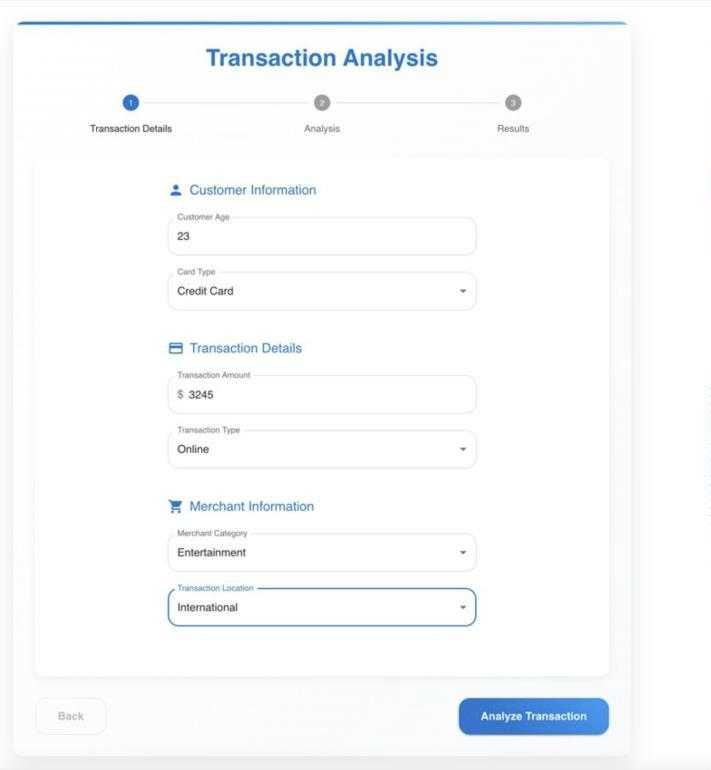
\includegraphics[width=256.25pt,height=277.46pt]{latexImage_0cd97b79fc5eb763f5a45a150ed4bf35.png}}
\end{picture}
\newpage
\begin{tikzpicture}[overlay]\path(0pt,0pt);\end{tikzpicture}
\begin{picture}(-5,0)(2.5,0)
\put(519.48,-97.53003){\fontsize{11}{1}\usefont{T1}{cmr}{m}{n}\selectfont\color{color_29791}  }
\put(473.45,-772.225){\fontsize{11}{1}\usefont{T1}{cmr}{m}{n}\selectfont\color{color_29791}15 | P a g e  }
\put(39.025,-788.725){\fontsize{11}{1}\usefont{T1}{cmr}{m}{n}\selectfont\color{color_29791} }
\put(48.65,-84.95){
\includegraphics[width=467.55pt,height=52.45pt]{latexImage_7044ae2d5aa88d56d597a9257795eea2.png}}
\end{picture}
\begin{tikzpicture}[overlay]
\path(0pt,0pt);
\filldraw[color_245272][even odd rule]
(37.55pt, -761.05pt) -- (527.85pt, -761.05pt)
 -- (527.85pt, -761.05pt)
 -- (527.85pt, -761.725pt)
 -- (527.85pt, -761.725pt)
 -- (37.55pt, -761.725pt)
 -- (37.55pt, -761.725pt)
 -- (37.55pt, -761.05pt)
;
\end{tikzpicture}
\begin{picture}(-5,0)(2.5,0)
\put(57.025,-114.28){\fontsize{14}{1}\usefont{T1}{cmr}{m}{n}\selectfont\color{color_29791}• Graphical User Interface (GUI): The GUI serves as the interface between the users }
\put(57.025,-131.05){\fontsize{14}{1}\usefont{T1}{cmr}{m}{n}\selectfont\color{color_29791}and the system. It provides a user-friendly environment for users to input }
\put(57.025,-147.8){\fontsize{14}{1}\usefont{T1}{cmr}{m}{n}\selectfont\color{color_29791}transaction details, view the data entered, and receive the system's predictions }
\put(57.025,-164.3){\fontsize{14}{1}\usefont{T1}{cmr}{m}{n}\selectfont\color{color_29791}regarding the possibility of fraudulent activity. }
\put(57.025,-195.8){\fontsize{14}{1}\usefont{T1}{cmr}{m}{n}\selectfont\color{color_29791} }
\put(57.025,-227.08){\fontsize{14}{1}\usefont{T1}{cmr}{m}{n}\selectfont\color{color_29791}• Fraud Detection Model: The core component of the system is the fraud detection }
\put(57.025,-243.83){\fontsize{14}{1}\usefont{T1}{cmr}{m}{n}\selectfont\color{color_29791}model. It is trained using logistic regression techniques and is responsible for }
\put(57.025,-260.58){\fontsize{14}{1}\usefont{T1}{cmr}{m}{n}\selectfont\color{color_29791}analyzing the input data to determine whether the transaction is fraudulent or }
\put(57.025,-277.32){\fontsize{14}{1}\usefont{T1}{cmr}{m}{n}\selectfont\color{color_29791}legitimate. The model utilizes data preprocessing techniques and logistic regression }
\put(57.025,-294.1){\fontsize{14}{1}\usefont{T1}{cmr}{m}{n}\selectfont\color{color_29791}to achieve accurate fraud detection. }
\put(57.025,-325.35){\fontsize{14}{1}\usefont{T1}{cmr}{m}{n}\selectfont\color{color_29791} }
\put(57.025,-356.6){\fontsize{14}{1}\usefont{T1}{cmr}{m}{n}\selectfont\color{color_29791}• Dataset: The dataset consists of real credit card transactions, including both }
\put(57.025,-373.37){\fontsize{14}{1}\usefont{T1}{cmr}{m}{n}\selectfont\color{color_29791}legitimate and fraudulent ones, used to train the fraud detection model. It serves as }
\put(57.025,-390.12){\fontsize{14}{1}\usefont{T1}{cmr}{m}{n}\selectfont\color{color_29791}the reference for the model to learn and differentiate between genuine and }
\put(57.025,-406.87){\fontsize{14}{1}\usefont{T1}{cmr}{m}{n}\selectfont\color{color_29791}fraudulent transactions. }
\put(57.025,-438.37){\fontsize{14}{1}\usefont{T1}{cmr}{m}{n}\selectfont\color{color_29791} }
\put(57.025,-469.65){\fontsize{14}{1}\usefont{T1}{cmr}{m}{n}\selectfont\color{color_29791}• Backend Processing: The backend processing component handles the }
\put(57.025,-486.4){\fontsize{14}{1}\usefont{T1}{cmr}{m}{n}\selectfont\color{color_29791}preprocessing of the transaction data, feeds it into the fraud detection model, and }
\put(57.025,-503.15){\fontsize{14}{1}\usefont{T1}{cmr}{m}{n}\selectfont\color{color_29791}processes the model's predictions to provide the final results to the users through the }
\put(57.025,-519.9){\fontsize{14}{1}\usefont{T1}{cmr}{m}{n}\selectfont\color{color_29791}GUI. }
\put(57.025,-551.17){\fontsize{14}{1}\usefont{T1}{cmr}{m}{n}\selectfont\color{color_29791} }
\put(57.025,-582.42){\fontsize{14}{1}\usefont{T1}{cmr}{m}{n}\selectfont\color{color_29791}By integrating these components and involving users as the primary users of the }
\put(57.025,-599.17){\fontsize{14}{1}\usefont{T1}{cmr}{m}{n}\selectfont\color{color_29791}system, the proposed Credit Card Fraud Detection using Logistic Regression aims }
\put(57.025,-615.93){\fontsize{14}{1}\usefont{T1}{cmr}{m}{n}\selectfont\color{color_29791}to provide an effective and user-friendly solution for detecting fraudulent credit }
\put(57.025,-632.7){\fontsize{14}{1}\usefont{T1}{cmr}{m}{n}\selectfont\color{color_29791}card transactions. }
\put(57.025,-663.95){\fontsize{14}{1}\usefont{T1}{cmr}{m}{n}\selectfont\color{color_29791} }
\put(38.275,-695.45){\fontsize{14}{1}\usefont{T1}{cmr}{b}{n}\selectfont\color{color_29791}4.2 PROPOSED SYSTEM ARCHITECTURE  }
\put(39.025,-718.72){\fontsize{14}{1}\usefont{T1}{cmr}{b}{n}\selectfont\color{color_29791}  }
\end{picture}
\newpage
\begin{tikzpicture}[overlay]\path(0pt,0pt);\end{tikzpicture}
\begin{picture}(-5,0)(2.5,0)
\put(519.48,-97.53003){\fontsize{11}{1}\usefont{T1}{cmr}{m}{n}\selectfont\color{color_29791}  }
\put(473.45,-772.225){\fontsize{11}{1}\usefont{T1}{cmr}{m}{n}\selectfont\color{color_29791}16 | P a g e  }
\put(39.025,-788.725){\fontsize{11}{1}\usefont{T1}{cmr}{m}{n}\selectfont\color{color_29791} }
\put(48.65,-84.95){
\includegraphics[width=467.55pt,height=52.45pt]{latexImage_7044ae2d5aa88d56d597a9257795eea2.png}}
\end{picture}
\begin{tikzpicture}[overlay]
\path(0pt,0pt);
\filldraw[color_245272][even odd rule]
(37.55pt, -761.05pt) -- (527.85pt, -761.05pt)
 -- (527.85pt, -761.05pt)
 -- (527.85pt, -761.725pt)
 -- (527.85pt, -761.725pt)
 -- (37.55pt, -761.725pt)
 -- (37.55pt, -761.725pt)
 -- (37.55pt, -761.05pt)
;
\end{tikzpicture}
\begin{picture}(-5,0)(2.5,0)
\put(38.275,-114.28){\fontsize{14}{1}\usefont{T1}{cmr}{m}{n}\selectfont\color{color_29791}The proposed system architecture for the Credit Card Fraud Detection project is }
\put(38.775,-137.8){\fontsize{14}{1}\usefont{T1}{cmr}{m}{n}\selectfont\color{color_29791}designed to effectively differentiate between legitimate and fraudulent transactions. The }
\put(38.775,-161.55){\fontsize{14}{1}\usefont{T1}{cmr}{m}{n}\selectfont\color{color_29791}architecture consists of several key components. Firstly, the user interacts with the }
\put(38.775,-185.05){\fontsize{14}{1}\usefont{T1}{cmr}{m}{n}\selectfont\color{color_29791}system through a user-friendly interface, entering the transaction details for fraud }
\put(38.775,-208.83){\fontsize{14}{1}\usefont{T1}{cmr}{m}{n}\selectfont\color{color_29791}detection. The input data is preprocessed using suitable techniques, such as }
\put(38.775,-232.58){\fontsize{14}{1}\usefont{T1}{cmr}{m}{n}\selectfont\color{color_29791}normalization, }
\put(39.025,-261.33){\fontsize{12}{1}\usefont{T1}{cmr}{m}{n}\selectfont\color{color_29791}  }
\put(500.48,-291.35){\fontsize{12}{1}\usefont{T1}{cmr}{m}{n}\selectfont\color{color_29791}  }
\put(170.33,-319.85){\fontsize{12}{1}\usefont{T1}{cmr}{b}{n}\selectfont\color{color_29791}FIGURE – 1 : SYSTEM ARCHITECTURE  }
\put(284.13,-347.6){\fontsize{12}{1}\usefont{T1}{cmr}{b}{n}\selectfont\color{color_29791}  }
\put(38.275,-380.12){\fontsize{14}{1}\usefont{T1}{cmr}{m}{n}\selectfont\color{color_29791}scaling, and handling missing values. Next, the logistic regression model is loaded, }
\put(38.775,-403.62){\fontsize{14}{1}\usefont{T1}{cmr}{m}{n}\selectfont\color{color_29791}which comprises multiple components to analyze the transaction data, including various }
\put(38.775,-427.37){\fontsize{14}{1}\usefont{T1}{cmr}{m}{n}\selectfont\color{color_29791}layers to process the attributes. The model is compiled with an appropriate optimizer, }
\put(38.775,-450.87){\fontsize{14}{1}\usefont{T1}{cmr}{m}{n}\selectfont\color{color_29791}loss function, and evaluation metrics. The trained model's weights are loaded, enabling }
\put(38.775,-474.65){\fontsize{14}{1}\usefont{T1}{cmr}{m}{n}\selectfont\color{color_29791}accurate fraud predictions. The system then predicts the likelihood of the transaction }
\put(38.775,-498.15){\fontsize{14}{1}\usefont{T1}{cmr}{m}{n}\selectfont\color{color_29791}being fraudulent, outputting the classification result as either "Fraud" or "Genuine."  }
\put(38.775,-521.9){\fontsize{14}{1}\usefont{T1}{cmr}{m}{n}\selectfont\color{color_29791}The proposed architecture ensures an efficient workflow, allowing users to assess the }
\put(38.775,-545.67){\fontsize{14}{1}\usefont{T1}{cmr}{m}{n}\selectfont\color{color_29791}authenticity of credit card transactions and contribute to the prevention of fraud. }
\put(38.275,-579.43){\fontsize{14}{1}\usefont{T1}{cmr}{b}{n}\selectfont\color{color_29791}4.3 UML DIAGRAMS  }
\put(38.275,-606.68){\fontsize{14}{1}\usefont{T1}{cmr}{b}{n}\selectfont\color{color_29791}4.3.1 USE CASE DIAGRAM  }
\put(38.275,-631.45){\fontsize{14}{1}\usefont{T1}{cmr}{m}{n}\selectfont\color{color_29791}In Figure 2, the design flow is clearly represented. Below is a description of the system }
\put(38.775,-648.2){\fontsize{14}{1}\usefont{T1}{cmr}{m}{n}\selectfont\color{color_29791}components and their roles: }
\put(57.025,-681.2){\fontsize{10}{1}\usefont{T1}{cmr}{m}{n}\selectfont\color{color_29791}• Transaction Input: This is the input module of the system, where transaction }
\put(75.05,-697.95){\fontsize{14}{1}\usefont{T1}{cmr}{m}{n}\selectfont\color{color_29791}details are submitted for fraud detection. These details may include information }
\put(75.05,-714.7){\fontsize{14}{1}\usefont{T1}{cmr}{m}{n}\selectfont\color{color_29791}like card number, transaction amount, and merchant details, sourced from e-}
\put(75.05,-731.47){\fontsize{14}{1}\usefont{T1}{cmr}{m}{n}\selectfont\color{color_29791}commerce platforms, banking systems, or payment gateways. }
\end{picture}
\newpage
\begin{tikzpicture}[overlay]\path(0pt,0pt);\end{tikzpicture}
\begin{picture}(-5,0)(2.5,0)
\put(519.48,-97.53003){\fontsize{11}{1}\usefont{T1}{cmr}{m}{n}\selectfont\color{color_29791}  }
\put(473.45,-772.225){\fontsize{11}{1}\usefont{T1}{cmr}{m}{n}\selectfont\color{color_29791}17 | P a g e  }
\put(39.025,-788.725){\fontsize{11}{1}\usefont{T1}{cmr}{m}{n}\selectfont\color{color_29791} }
\put(48.65,-84.95){
\includegraphics[width=467.55pt,height=52.45pt]{latexImage_7044ae2d5aa88d56d597a9257795eea2.png}}
\end{picture}
\begin{tikzpicture}[overlay]
\path(0pt,0pt);
\filldraw[color_245272][even odd rule]
(37.55pt, -761.05pt) -- (527.85pt, -761.05pt)
 -- (527.85pt, -761.05pt)
 -- (527.85pt, -761.725pt)
 -- (527.85pt, -761.725pt)
 -- (37.55pt, -761.725pt)
 -- (37.55pt, -761.725pt)
 -- (37.55pt, -761.05pt)
;
\end{tikzpicture}
\begin{picture}(-5,0)(2.5,0)
\put(57.025,-114.28){\fontsize{10}{1}\usefont{T1}{cmr}{m}{n}\selectfont\color{color_29791}• Preprocessing: In this module, the transaction data is preprocessed and prepared }
\put(75.05,-131.05){\fontsize{14}{1}\usefont{T1}{cmr}{m}{n}\selectfont\color{color_29791}for analysis. This may involve normalizing numerical values, handling missing }
\put(75.05,-147.8){\fontsize{14}{1}\usefont{T1}{cmr}{m}{n}\selectfont\color{color_29791}data, or other steps that ensure the data is in the right format for analysis. }
\put(57.025,-180.55){\fontsize{10}{1}\usefont{T1}{cmr}{m}{n}\selectfont\color{color_29791}• Feature Extraction: In this module, the system extracts relevant features from }
\put(75.05,-197.3){\fontsize{14}{1}\usefont{T1}{cmr}{m}{n}\selectfont\color{color_29791}the transaction data that will be used for detection. These features may include }
\put(75.05,-214.08){\fontsize{14}{1}\usefont{T1}{cmr}{m}{n}\selectfont\color{color_29791}transaction amount, frequency, user behavior patterns, and merchant details. }
\put(57.025,-247.08){\fontsize{10}{1}\usefont{T1}{cmr}{m}{n}\selectfont\color{color_29791}• Machine Learning Model: This is the core of the system, where a logistic }
\put(75.05,-263.82){\fontsize{14}{1}\usefont{T1}{cmr}{m}{n}\selectfont\color{color_29791}regression model is used to analyze the extracted features and compare them to }
\put(75.05,-280.57){\fontsize{14}{1}\usefont{T1}{cmr}{m}{n}\selectfont\color{color_29791}patterns of legitimate transactions. The model is trained to recognize patterns }
\put(75.05,-297.35){\fontsize{14}{1}\usefont{T1}{cmr}{m}{n}\selectfont\color{color_29791}indicative of fraudulent activity. }
\put(57.025,-330.35){\fontsize{10}{1}\usefont{T1}{cmr}{m}{n}\selectfont\color{color_29791}• Decision Making: Based on the output of the logistic regression model, the }
\put(75.05,-347.1){\fontsize{14}{1}\usefont{T1}{cmr}{m}{n}\selectfont\color{color_29791}system makes a decision about the transaction's authenticity. If the transaction is }
\put(75.05,-363.85){\fontsize{14}{1}\usefont{T1}{cmr}{m}{n}\selectfont\color{color_29791}classified as fraudulent, it is flagged for further investigation or immediate action. }
\put(57.025,-396.87){\fontsize{10}{1}\usefont{T1}{cmr}{m}{n}\selectfont\color{color_29791}• Output: The final output of the system is a decision about the transaction’s }
\put(75.05,-413.62){\fontsize{14}{1}\usefont{T1}{cmr}{m}{n}\selectfont\color{color_29791}authenticity, along with a probability score indicating the likelihood of fraud. This }
\put(75.05,-430.37){\fontsize{14}{1}\usefont{T1}{cmr}{m}{n}\selectfont\color{color_29791}output may be presented to users (e.g., bank representatives) or used to trigger }
\put(75.05,-447.12){\fontsize{14}{1}\usefont{T1}{cmr}{m}{n}\selectfont\color{color_29791}further actions within other systems. }
\put(38.275,-479.9){\fontsize{14}{1}\usefont{T1}{cmr}{m}{n}\selectfont\color{color_29791}  }
\put(39.025,-512.9){\fontsize{16}{1}\usefont{T1}{cmr}{m}{n}\selectfont\color{color_29791}  }
\end{picture}
\newpage
\begin{tikzpicture}[overlay]\path(0pt,0pt);\end{tikzpicture}
\begin{picture}(-5,0)(2.5,0)
\put(519.48,-97.53003){\fontsize{11}{1}\usefont{T1}{cmr}{m}{n}\selectfont\color{color_29791}  }
\put(473.45,-772.225){\fontsize{11}{1}\usefont{T1}{cmr}{m}{n}\selectfont\color{color_29791}18 | P a g e  }
\put(39.025,-788.725){\fontsize{11}{1}\usefont{T1}{cmr}{m}{n}\selectfont\color{color_29791} }
\put(48.65,-84.95){
\includegraphics[width=467.55pt,height=52.45pt]{latexImage_7044ae2d5aa88d56d597a9257795eea2.png}}
\end{picture}
\begin{tikzpicture}[overlay]
\path(0pt,0pt);
\filldraw[color_245272][even odd rule]
(37.55pt, -761.05pt) -- (527.85pt, -761.05pt)
 -- (527.85pt, -761.05pt)
 -- (527.85pt, -761.725pt)
 -- (527.85pt, -761.725pt)
 -- (37.55pt, -761.725pt)
 -- (37.55pt, -761.725pt)
 -- (37.55pt, -761.05pt)
;
\end{tikzpicture}
\begin{picture}(-5,0)(2.5,0)
\put(472.45,-352.85){\fontsize{14}{1}\usefont{T1}{cmr}{m}{n}\selectfont\color{color_29791}  }
\put(138.08,-376.62){\fontsize{12}{1}\usefont{T1}{cmr}{b}{n}\selectfont\color{color_29791}FIGURE – 2 : DESIGN FLOW OF Fraud DETECTION  }
\put(39.025,-408.37){\fontsize{14}{1}\usefont{T1}{cmr}{b}{n}\selectfont\color{color_29791}  }
\put(38.275,-442.87){\fontsize{14}{1}\usefont{T1}{cmr}{b}{n}\selectfont\color{color_29791}4.3.2 SEQUENCE DIAGRAM  }
\put(39.025,-474.15){\fontsize{14}{1}\usefont{T1}{cmr}{b}{n}\selectfont\color{color_29791}  }
\put(38.275,-508.15){\fontsize{14}{1}\usefont{T1}{cmr}{b}{n}\selectfont\color{color_29791}The sequence of events for the Credit Card Fraud Detection system: }
\put(57.025,-536.4){\fontsize{14}{1}\usefont{T1}{cmr}{m}{n}\selectfont\color{color_29791}1. User Input: The user initiates the fraud detection process by entering details }
\put(75.05,-560.17){\fontsize{14}{1}\usefont{T1}{cmr}{m}{n}\selectfont\color{color_29791}about a credit card transaction (e.g., transaction amount, user location, etc.). }
\put(57.025,-588.43){\fontsize{14}{1}\usefont{T1}{cmr}{m}{n}\selectfont\color{color_29791}2. Data Validation: The system receives the input data and validates it to ensure it }
\put(75.05,-612.17){\fontsize{14}{1}\usefont{T1}{cmr}{m}{n}\selectfont\color{color_29791}is properly formatted and contains all necessary information. }
\put(57.025,-640.45){\fontsize{14}{1}\usefont{T1}{cmr}{m}{n}\selectfont\color{color_29791}3. Feature Extraction: The system extracts relevant features from the transaction }
\put(75.05,-663.95){\fontsize{14}{1}\usefont{T1}{cmr}{m}{n}\selectfont\color{color_29791}details (e.g., transaction amount, time, and user behavior). }
\put(57.025,-692.45){\fontsize{14}{1}\usefont{T1}{cmr}{m}{n}\selectfont\color{color_29791}4. Preprocessing: The system preprocesses the transaction data by normalizing or }
\put(75.05,-715.95){\fontsize{14}{1}\usefont{T1}{cmr}{m}{n}\selectfont\color{color_29791}s}
\put(100.75,-352.48){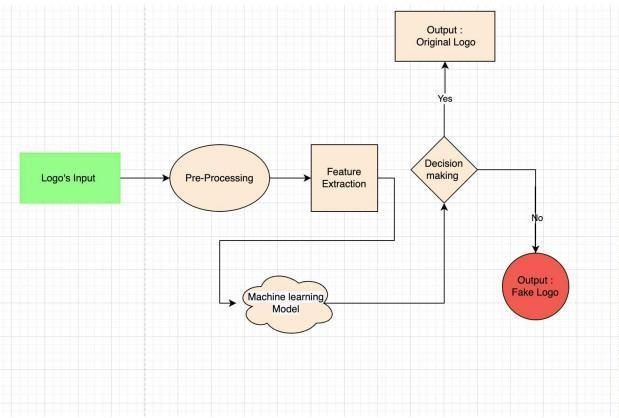
\includegraphics[width=371.4pt,height=250.8pt]{latexImage_3fcfd75b11393531efcbdf7b69970cdb.png}}
\end{picture}
\newpage
\begin{tikzpicture}[overlay]\path(0pt,0pt);\end{tikzpicture}
\begin{picture}(-5,0)(2.5,0)
\put(519.48,-97.53003){\fontsize{11}{1}\usefont{T1}{cmr}{m}{n}\selectfont\color{color_29791}  }
\put(473.45,-772.225){\fontsize{11}{1}\usefont{T1}{cmr}{m}{n}\selectfont\color{color_29791}19 | P a g e  }
\put(39.025,-788.725){\fontsize{11}{1}\usefont{T1}{cmr}{m}{n}\selectfont\color{color_29791} }
\put(48.65,-84.95){
\includegraphics[width=467.55pt,height=52.45pt]{latexImage_7044ae2d5aa88d56d597a9257795eea2.png}}
\end{picture}
\begin{tikzpicture}[overlay]
\path(0pt,0pt);
\filldraw[color_245272][even odd rule]
(37.55pt, -761.05pt) -- (527.85pt, -761.05pt)
 -- (527.85pt, -761.05pt)
 -- (527.85pt, -761.725pt)
 -- (527.85pt, -761.725pt)
 -- (37.55pt, -761.725pt)
 -- (37.55pt, -761.725pt)
 -- (37.55pt, -761.05pt)
;
\end{tikzpicture}
\begin{picture}(-5,0)(2.5,0)
\put(57.025,-114.28){\fontsize{14}{1}\usefont{T1}{cmr}{m}{n}\selectfont\color{color_29791}5. Model Prediction: The preprocessed data is passed through the trained fraud }
\put(75.05,-137.8){\fontsize{14}{1}\usefont{T1}{cmr}{m}{n}\selectfont\color{color_29791}detection model. }
\put(57.025,-166.05){\fontsize{14}{1}\usefont{T1}{cmr}{m}{n}\selectfont\color{color_29791}6. Generate Prediction: The model analyzes the data and generates predictions on }
\put(75.05,-189.8){\fontsize{14}{1}\usefont{T1}{cmr}{m}{n}\selectfont\color{color_29791}whether the transaction is legitimate or fraudulent. }
\put(57.025,-218.08){\fontsize{14}{1}\usefont{T1}{cmr}{m}{n}\selectfont\color{color_29791}7. Receive Prediction Results: The system receives the prediction results from the }
\put(75.05,-241.83){\fontsize{14}{1}\usefont{T1}{cmr}{m}{n}\selectfont\color{color_29791}model. }
\put(57.025,-270.07){\fontsize{14}{1}\usefont{T1}{cmr}{m}{n}\selectfont\color{color_29791}8. Output the Result: The system sends the fraud detection result to the user or }
\put(75.05,-293.85){\fontsize{14}{1}\usefont{T1}{cmr}{m}{n}\selectfont\color{color_29791}relevant system, indicating whether the transaction is classified as fraudulent or }
\put(75.05,-317.35){\fontsize{14}{1}\usefont{T1}{cmr}{m}{n}\selectfont\color{color_29791}not. }
\put(57.025,-345.6){\fontsize{14}{1}\usefont{T1}{cmr}{m}{n}\selectfont\color{color_29791}9. User Receives Result: The user or administrator receives the fraud detection }
\put(75.05,-369.35){\fontsize{14}{1}\usefont{T1}{cmr}{m}{n}\selectfont\color{color_29791}result from the system. }
\put(57.025,-397.62){\fontsize{14}{1}\usefont{T1}{cmr}{m}{n}\selectfont\color{color_29791}10. Repeat Process: The process repeats as the user can initiate fraud detection for }
\put(75.05,-421.37){\fontsize{14}{1}\usefont{T1}{cmr}{m}{n}\selectfont\color{color_29791}additional transactions. }
\put(38.275,-449.62){\fontsize{14}{1}\usefont{T1}{cmr}{m}{n}\selectfont\color{color_29791} Please note that a sequence diagram is typically created using diagramming tools or }
\put(38.775,-473.15){\fontsize{14}{1}\usefont{T1}{cmr}{m}{n}\selectfont\color{color_29791}software such as UML tools (e.g., Lucidchart, Draw.io, Visual Paradigm) to provide a }
\put(38.775,-496.9){\fontsize{14}{1}\usefont{T1}{cmr}{m}{n}\selectfont\color{color_29791}visual representation of the sequence of interactions between objects and components }
\put(38.775,-520.65){\fontsize{14}{1}\usefont{T1}{cmr}{m}{n}\selectfont\color{color_29791}in the system, allowing for better understanding of the flow of actions in the credit card }
\put(38.775,-544.15){\fontsize{14}{1}\usefont{T1}{cmr}{b}{n}\selectfont\color{color_29791}fraud detection process. }
\put(386.18,-699.2){\fontsize{12}{1}\usefont{T1}{cmr}{b}{n}\selectfont\color{color_29791}  }
\put(184.83,-724.72){\fontsize{12}{1}\usefont{T1}{cmr}{b}{n}\selectfont\color{color_29791}FIGURE-3 : SEQUENCE DIAGRAM  }
\put(39.025,-752.225){\fontsize{14}{1}\usefont{T1}{cmr}{b}{n}\selectfont\color{color_29791} }
\put(182.2,-699.09){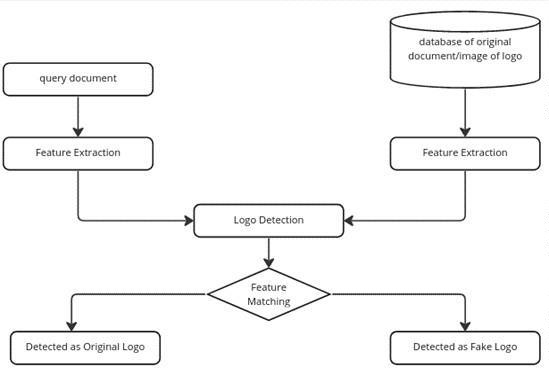
\includegraphics[width=203.9pt,height=139.27pt]{latexImage_77cf61ceee649bcd16e1f315975a1757.png}}
\end{picture}
\newpage
\begin{tikzpicture}[overlay]\path(0pt,0pt);\end{tikzpicture}
\begin{picture}(-5,0)(2.5,0)
\put(519.48,-97.53003){\fontsize{11}{1}\usefont{T1}{cmr}{m}{n}\selectfont\color{color_29791}  }
\put(473.45,-772.225){\fontsize{11}{1}\usefont{T1}{cmr}{m}{n}\selectfont\color{color_29791}20 | P a g e  }
\put(39.025,-788.725){\fontsize{11}{1}\usefont{T1}{cmr}{m}{n}\selectfont\color{color_29791} }
\put(48.65,-84.95){
\includegraphics[width=467.55pt,height=52.45pt]{latexImage_7044ae2d5aa88d56d597a9257795eea2.png}}
\end{picture}
\begin{tikzpicture}[overlay]
\path(0pt,0pt);
\filldraw[color_245272][even odd rule]
(37.55pt, -761.05pt) -- (527.85pt, -761.05pt)
 -- (527.85pt, -761.05pt)
 -- (527.85pt, -761.725pt)
 -- (527.85pt, -761.725pt)
 -- (37.55pt, -761.725pt)
 -- (37.55pt, -761.725pt)
 -- (37.55pt, -761.05pt)
;
\end{tikzpicture}
\begin{picture}(-5,0)(2.5,0)
\put(39.025,-114.28){\fontsize{14}{1}\usefont{T1}{cmr}{b}{n}\selectfont\color{color_29791}  }
\put(243.35,-141.55){\fontsize{14}{1}\usefont{T1}{cmr}{b}{n}\selectfont\color{color_29791}CHAPTER 5  }
\put(217.1,-169.05){\fontsize{14}{1}\usefont{T1}{cmr}{b}{n}\selectfont\color{color_29791}IMPLEMENTATION  }
\end{picture}
\begin{tikzpicture}[overlay]
\path(0pt,0pt);
\filldraw[color_29791][even odd rule]
(217.1pt, -171.8pt) -- (348.65pt, -171.8pt)
 -- (348.65pt, -171.8pt)
 -- (348.65pt, -170.55pt)
 -- (348.65pt, -170.55pt)
 -- (217.1pt, -170.55pt) -- cycle
;
\end{tikzpicture}
\begin{picture}(-5,0)(2.5,0)
\put(284.38,-193.55){\fontsize{14}{1}\usefont{T1}{cmr}{b}{n}\selectfont\color{color_29791}  }
\put(38.275,-220.83){\fontsize{14}{1}\usefont{T1}{cmr}{b}{n}\selectfont\color{color_29791}5.1 Source Code  }
\put(39.025,-245.58){\fontsize{14}{1}\usefont{T1}{cmr}{b}{n}\selectfont\color{color_29791}  }
\put(38.275,-272.82){\fontsize{14}{1}\usefont{T1}{cmr}{b}{n}\selectfont\color{color_29791}Main Code Python File :  }
\put(39.025,-297.6){\fontsize{14}{1}\usefont{T1}{cmr}{b}{n}\selectfont\color{color_29791}  }
\put(39.025,-331.6){\fontsize{14}{1}\usefont{T1}{cmr}{m}{n}\selectfont\color{color_29791}from flask import Flask, request, jsonify }
\put(39.025,-365.85){\fontsize{14}{1}\usefont{T1}{cmr}{m}{n}\selectfont\color{color_29791}from flask\_cors import CORS }
\put(39.025,-400.12){\fontsize{14}{1}\usefont{T1}{cmr}{m}{n}\selectfont\color{color_29791}import numpy as np }
\put(39.025,-434.37){\fontsize{14}{1}\usefont{T1}{cmr}{m}{n}\selectfont\color{color_29791}import hashlib }
\put(39.025,-468.65){\fontsize{14}{1}\usefont{T1}{cmr}{m}{n}\selectfont\color{color_29791}import logging }
\put(39.025,-502.9){\fontsize{14}{1}\usefont{T1}{cmr}{m}{n}\selectfont\color{color_29791}import time }
\put(39.025,-537.15){\fontsize{14}{1}\usefont{T1}{cmr}{m}{n}\selectfont\color{color_29791}from datetime import datetime }
\put(39.025,-571.42){\fontsize{14}{1}\usefont{T1}{cmr}{m}{n}\selectfont\color{color_29791} }
\put(39.025,-605.67){\fontsize{14}{1}\usefont{T1}{cmr}{m}{n}\selectfont\color{color_29791}\# Configure logging }
\put(39.025,-639.7){\fontsize{14}{1}\usefont{T1}{cmr}{m}{n}\selectfont\color{color_29791}logging.basicConfig(level=logging.INFO) }
\put(39.025,-673.95){\fontsize{14}{1}\usefont{T1}{cmr}{m}{n}\selectfont\color{color_29791}logger = logging.getLogger(\_\_name\_\_) }
\put(39.025,-708.2){\fontsize{14}{1}\usefont{T1}{cmr}{m}{n}\selectfont\color{color_29791} }
\put(39.025,-742.475){\fontsize{14}{1}\usefont{T1}{cmr}{m}{n}\selectfont\color{color_29791}app = Flask(\_\_name\_\_) }
\end{picture}
\newpage
\begin{tikzpicture}[overlay]\path(0pt,0pt);\end{tikzpicture}
\begin{picture}(-5,0)(2.5,0)
\put(519.48,-97.53003){\fontsize{11}{1}\usefont{T1}{cmr}{m}{n}\selectfont\color{color_29791}  }
\put(473.45,-772.225){\fontsize{11}{1}\usefont{T1}{cmr}{m}{n}\selectfont\color{color_29791}21 | P a g e  }
\put(39.025,-788.725){\fontsize{11}{1}\usefont{T1}{cmr}{m}{n}\selectfont\color{color_29791} }
\put(48.65,-84.95){
\includegraphics[width=467.55pt,height=52.45pt]{latexImage_7044ae2d5aa88d56d597a9257795eea2.png}}
\end{picture}
\begin{tikzpicture}[overlay]
\path(0pt,0pt);
\filldraw[color_245272][even odd rule]
(37.55pt, -761.05pt) -- (527.85pt, -761.05pt)
 -- (527.85pt, -761.05pt)
 -- (527.85pt, -761.725pt)
 -- (527.85pt, -761.725pt)
 -- (37.55pt, -761.725pt)
 -- (37.55pt, -761.725pt)
 -- (37.55pt, -761.05pt)
;
\end{tikzpicture}
\begin{picture}(-5,0)(2.5,0)
\put(39.025,-114.28){\fontsize{14}{1}\usefont{T1}{cmr}{m}{n}\selectfont\color{color_29791}CORS(app) }
\put(39.025,-148.55){\fontsize{14}{1}\usefont{T1}{cmr}{m}{n}\selectfont\color{color_29791} }
\put(39.025,-182.8){\fontsize{14}{1}\usefont{T1}{cmr}{m}{n}\selectfont\color{color_29791}def predict\_fraud(amount, transaction\_type, merchant\_category, card\_type, }
\put(39.025,-199.3){\fontsize{14}{1}\usefont{T1}{cmr}{m}{n}\selectfont\color{color_29791}transaction\_location, customer\_age): }
\put(39.025,-233.58){\fontsize{14}{1}\usefont{T1}{cmr}{m}{n}\selectfont\color{color_29791}    """ }
\put(39.025,-267.82){\fontsize{14}{1}\usefont{T1}{cmr}{m}{n}\selectfont\color{color_29791}    Predict fraud based on transaction features: }
\put(39.025,-302.1){\fontsize{14}{1}\usefont{T1}{cmr}{m}{n}\selectfont\color{color_29791}    - amount: Transaction amount }
\put(39.025,-336.35){\fontsize{14}{1}\usefont{T1}{cmr}{m}{n}\selectfont\color{color_29791}    - transaction\_type: Type of transaction (online/in-store/atm/international) }
\put(39.025,-370.6){\fontsize{14}{1}\usefont{T1}{cmr}{m}{n}\selectfont\color{color_29791}    - merchant\_category: Category of merchant }
\put(39.025,-404.87){\fontsize{14}{1}\usefont{T1}{cmr}{m}{n}\selectfont\color{color_29791}    - card\_type: Type of card (credit/debit/prepaid) }
\put(39.025,-439.12){\fontsize{14}{1}\usefont{T1}{cmr}{m}{n}\selectfont\color{color_29791}    - transaction\_location: Location of transaction (domestic/international/online) }
\put(39.025,-473.4){\fontsize{14}{1}\usefont{T1}{cmr}{m}{n}\selectfont\color{color_29791}    - customer\_age: Age of the customer }
\put(39.025,-507.65){\fontsize{14}{1}\usefont{T1}{cmr}{m}{n}\selectfont\color{color_29791}    """ }
\put(39.025,-541.9){\fontsize{14}{1}\usefont{T1}{cmr}{m}{n}\selectfont\color{color_29791}    \# Create a deterministic hash based on input features }
\put(39.025,-576.17){\fontsize{14}{1}\usefont{T1}{cmr}{m}{n}\selectfont\color{color_29791}    input\_str = }
\put(39.025,-592.93){\fontsize{14}{1}\usefont{T1}{cmr}{m}{n}\selectfont\color{color_29791}f"\{amount\}\_\{transaction\_type\}\_\{merchant\_category\}\_\{card\_type\}\_\{transaction\_loca}
\put(39.025,-609.67){\fontsize{14}{1}\usefont{T1}{cmr}{m}{n}\selectfont\color{color_29791}tion\}\_\{customer\_age\}" }
\put(39.025,-643.7){\fontsize{14}{1}\usefont{T1}{cmr}{m}{n}\selectfont\color{color_29791}    hash\_value = int(hashlib.md5(input\_str.encode()).hexdigest(), 16) }
\put(39.025,-677.95){\fontsize{14}{1}\usefont{T1}{cmr}{m}{n}\selectfont\color{color_29791}     }
\put(39.025,-712.2){\fontsize{14}{1}\usefont{T1}{cmr}{m}{n}\selectfont\color{color_29791}    \# Base fraud probability }
\put(39.025,-746.475){\fontsize{14}{1}\usefont{T1}{cmr}{m}{n}\selectfont\color{color_29791}    base\_prob = 0.1 }
\end{picture}
\newpage
\begin{tikzpicture}[overlay]\path(0pt,0pt);\end{tikzpicture}
\begin{picture}(-5,0)(2.5,0)
\put(519.48,-97.53003){\fontsize{11}{1}\usefont{T1}{cmr}{m}{n}\selectfont\color{color_29791}  }
\put(473.45,-772.225){\fontsize{11}{1}\usefont{T1}{cmr}{m}{n}\selectfont\color{color_29791}22 | P a g e  }
\put(39.025,-788.725){\fontsize{11}{1}\usefont{T1}{cmr}{m}{n}\selectfont\color{color_29791} }
\put(48.65,-84.95){
\includegraphics[width=467.55pt,height=52.45pt]{latexImage_7044ae2d5aa88d56d597a9257795eea2.png}}
\end{picture}
\begin{tikzpicture}[overlay]
\path(0pt,0pt);
\filldraw[color_245272][even odd rule]
(37.55pt, -761.05pt) -- (527.85pt, -761.05pt)
 -- (527.85pt, -761.05pt)
 -- (527.85pt, -761.725pt)
 -- (527.85pt, -761.725pt)
 -- (37.55pt, -761.725pt)
 -- (37.55pt, -761.725pt)
 -- (37.55pt, -761.05pt)
;
\end{tikzpicture}
\begin{picture}(-5,0)(2.5,0)
\put(39.025,-114.28){\fontsize{14}{1}\usefont{T1}{cmr}{m}{n}\selectfont\color{color_29791}     }
\put(39.025,-148.55){\fontsize{14}{1}\usefont{T1}{cmr}{m}{n}\selectfont\color{color_29791}    \# Adjust probability based on amount }
\put(39.025,-182.8){\fontsize{14}{1}\usefont{T1}{cmr}{m}{n}\selectfont\color{color_29791}    if amount > 1000: }
\put(39.025,-216.83){\fontsize{14}{1}\usefont{T1}{cmr}{m}{n}\selectfont\color{color_29791}        base\_prob += 0.2 }
\put(39.025,-251.08){\fontsize{14}{1}\usefont{T1}{cmr}{m}{n}\selectfont\color{color_29791}    elif amount > 500: }
\put(39.025,-285.33){\fontsize{14}{1}\usefont{T1}{cmr}{m}{n}\selectfont\color{color_29791}        base\_prob += 0.1 }
\put(39.025,-319.6){\fontsize{14}{1}\usefont{T1}{cmr}{m}{n}\selectfont\color{color_29791}     }
\put(39.025,-353.85){\fontsize{14}{1}\usefont{T1}{cmr}{m}{n}\selectfont\color{color_29791}    \# Adjust based on transaction type }
\put(39.025,-388.12){\fontsize{14}{1}\usefont{T1}{cmr}{m}{n}\selectfont\color{color_29791}    if transaction\_type.lower() == 'online': }
\put(39.025,-422.37){\fontsize{14}{1}\usefont{T1}{cmr}{m}{n}\selectfont\color{color_29791}        base\_prob += 0.15 }
\put(39.025,-456.62){\fontsize{14}{1}\usefont{T1}{cmr}{m}{n}\selectfont\color{color_29791}    elif transaction\_type.lower() == 'international': }
\put(39.025,-490.9){\fontsize{14}{1}\usefont{T1}{cmr}{m}{n}\selectfont\color{color_29791}        base\_prob += 0.2 }
\put(39.025,-525.15){\fontsize{14}{1}\usefont{T1}{cmr}{m}{n}\selectfont\color{color_29791}    elif transaction\_type.lower() == 'atm': }
\put(39.025,-559.42){\fontsize{14}{1}\usefont{T1}{cmr}{m}{n}\selectfont\color{color_29791}        base\_prob += 0.1 }
\put(39.025,-593.67){\fontsize{14}{1}\usefont{T1}{cmr}{m}{n}\selectfont\color{color_29791}     }
\put(39.025,-627.92){\fontsize{14}{1}\usefont{T1}{cmr}{m}{n}\selectfont\color{color_29791}    \# Adjust based on card type }
\put(39.025,-662.2){\fontsize{14}{1}\usefont{T1}{cmr}{m}{n}\selectfont\color{color_29791}    if card\_type.lower() == 'prepaid': }
\put(39.025,-696.2){\fontsize{14}{1}\usefont{T1}{cmr}{m}{n}\selectfont\color{color_29791}        base\_prob += 0.15 }
\put(39.025,-730.48){\fontsize{14}{1}\usefont{T1}{cmr}{m}{n}\selectfont\color{color_29791}    elif card\_type.lower() == 'debit': }
\end{picture}
\newpage
\begin{tikzpicture}[overlay]\path(0pt,0pt);\end{tikzpicture}
\begin{picture}(-5,0)(2.5,0)
\put(519.48,-97.53003){\fontsize{11}{1}\usefont{T1}{cmr}{m}{n}\selectfont\color{color_29791}  }
\put(473.45,-772.225){\fontsize{11}{1}\usefont{T1}{cmr}{m}{n}\selectfont\color{color_29791}23 | P a g e  }
\put(39.025,-788.725){\fontsize{11}{1}\usefont{T1}{cmr}{m}{n}\selectfont\color{color_29791} }
\put(48.65,-84.95){
\includegraphics[width=467.55pt,height=52.45pt]{latexImage_7044ae2d5aa88d56d597a9257795eea2.png}}
\end{picture}
\begin{tikzpicture}[overlay]
\path(0pt,0pt);
\filldraw[color_245272][even odd rule]
(37.55pt, -761.05pt) -- (527.85pt, -761.05pt)
 -- (527.85pt, -761.05pt)
 -- (527.85pt, -761.725pt)
 -- (527.85pt, -761.725pt)
 -- (37.55pt, -761.725pt)
 -- (37.55pt, -761.725pt)
 -- (37.55pt, -761.05pt)
;
\end{tikzpicture}
\begin{picture}(-5,0)(2.5,0)
\put(39.025,-114.28){\fontsize{14}{1}\usefont{T1}{cmr}{m}{n}\selectfont\color{color_29791}        base\_prob += 0.05 }
\put(39.025,-148.55){\fontsize{14}{1}\usefont{T1}{cmr}{m}{n}\selectfont\color{color_29791}     }
\put(39.025,-182.8){\fontsize{14}{1}\usefont{T1}{cmr}{m}{n}\selectfont\color{color_29791}    \# Adjust based on transaction location }
\put(39.025,-216.83){\fontsize{14}{1}\usefont{T1}{cmr}{m}{n}\selectfont\color{color_29791}    if transaction\_location.lower() == 'international': }
\put(39.025,-251.08){\fontsize{14}{1}\usefont{T1}{cmr}{m}{n}\selectfont\color{color_29791}        base\_prob += 0.15 }
\put(39.025,-285.33){\fontsize{14}{1}\usefont{T1}{cmr}{m}{n}\selectfont\color{color_29791}    elif transaction\_location.lower() == 'online': }
\put(39.025,-319.6){\fontsize{14}{1}\usefont{T1}{cmr}{m}{n}\selectfont\color{color_29791}        base\_prob += 0.1 }
\put(39.025,-353.85){\fontsize{14}{1}\usefont{T1}{cmr}{m}{n}\selectfont\color{color_29791}     }
\put(39.025,-388.12){\fontsize{14}{1}\usefont{T1}{cmr}{m}{n}\selectfont\color{color_29791}    \# Adjust based on customer age }
\put(39.025,-422.37){\fontsize{14}{1}\usefont{T1}{cmr}{m}{n}\selectfont\color{color_29791}    try: }
\put(39.025,-456.62){\fontsize{14}{1}\usefont{T1}{cmr}{m}{n}\selectfont\color{color_29791}        age = int(customer\_age) }
\put(39.025,-490.9){\fontsize{14}{1}\usefont{T1}{cmr}{m}{n}\selectfont\color{color_29791}        if age < 25 or age > 75: }
\put(39.025,-525.15){\fontsize{14}{1}\usefont{T1}{cmr}{m}{n}\selectfont\color{color_29791}            base\_prob += 0.1 }
\put(39.025,-559.42){\fontsize{14}{1}\usefont{T1}{cmr}{m}{n}\selectfont\color{color_29791}    except ValueError: }
\put(39.025,-593.67){\fontsize{14}{1}\usefont{T1}{cmr}{m}{n}\selectfont\color{color_29791}        pass }
\put(39.025,-627.92){\fontsize{14}{1}\usefont{T1}{cmr}{m}{n}\selectfont\color{color_29791}     }
\put(39.025,-662.2){\fontsize{14}{1}\usefont{T1}{cmr}{m}{n}\selectfont\color{color_29791}    \# Adjust based on merchant category }
\put(39.025,-696.2){\fontsize{14}{1}\usefont{T1}{cmr}{m}{n}\selectfont\color{color_29791}    high\_risk\_categories = ['electronics', 'travel', 'entertainment'] }
\put(39.025,-730.48){\fontsize{14}{1}\usefont{T1}{cmr}{m}{n}\selectfont\color{color_29791}    if merchant\_category.lower() in high\_risk\_categories: }
\end{picture}
\newpage
\begin{tikzpicture}[overlay]\path(0pt,0pt);\end{tikzpicture}
\begin{picture}(-5,0)(2.5,0)
\put(519.48,-97.53003){\fontsize{11}{1}\usefont{T1}{cmr}{m}{n}\selectfont\color{color_29791}  }
\put(473.45,-772.225){\fontsize{11}{1}\usefont{T1}{cmr}{m}{n}\selectfont\color{color_29791}24 | P a g e  }
\put(39.025,-788.725){\fontsize{11}{1}\usefont{T1}{cmr}{m}{n}\selectfont\color{color_29791} }
\put(48.65,-84.95){
\includegraphics[width=467.55pt,height=52.45pt]{latexImage_7044ae2d5aa88d56d597a9257795eea2.png}}
\end{picture}
\begin{tikzpicture}[overlay]
\path(0pt,0pt);
\filldraw[color_245272][even odd rule]
(37.55pt, -761.05pt) -- (527.85pt, -761.05pt)
 -- (527.85pt, -761.05pt)
 -- (527.85pt, -761.725pt)
 -- (527.85pt, -761.725pt)
 -- (37.55pt, -761.725pt)
 -- (37.55pt, -761.725pt)
 -- (37.55pt, -761.05pt)
;
\end{tikzpicture}
\begin{picture}(-5,0)(2.5,0)
\put(39.025,-114.28){\fontsize{14}{1}\usefont{T1}{cmr}{m}{n}\selectfont\color{color_29791}        base\_prob += 0.1 }
\put(39.025,-148.55){\fontsize{14}{1}\usefont{T1}{cmr}{m}{n}\selectfont\color{color_29791}     }
\put(39.025,-182.8){\fontsize{14}{1}\usefont{T1}{cmr}{m}{n}\selectfont\color{color_29791}    \# Use hash to add some randomness while keeping it consistent for same inputs }
\put(39.025,-216.83){\fontsize{14}{1}\usefont{T1}{cmr}{m}{n}\selectfont\color{color_29791}    hash\_factor = (hash\_value \% 100) / 1000 }
\put(39.025,-251.08){\fontsize{14}{1}\usefont{T1}{cmr}{m}{n}\selectfont\color{color_29791}    final\_prob = min(0.99, base\_prob + hash\_factor) }
\put(39.025,-285.33){\fontsize{14}{1}\usefont{T1}{cmr}{m}{n}\selectfont\color{color_29791}     }
\put(39.025,-319.6){\fontsize{14}{1}\usefont{T1}{cmr}{m}{n}\selectfont\color{color_29791}    \# Determine if it's fraud based on probability threshold }
\put(39.025,-353.85){\fontsize{14}{1}\usefont{T1}{cmr}{m}{n}\selectfont\color{color_29791}    is\_fraud = final\_prob > 0.5 }
\put(39.025,-388.12){\fontsize{14}{1}\usefont{T1}{cmr}{m}{n}\selectfont\color{color_29791}     }
\put(39.025,-422.37){\fontsize{14}{1}\usefont{T1}{cmr}{m}{n}\selectfont\color{color_29791}    return is\_fraud, final\_prob }
\put(39.025,-456.62){\fontsize{14}{1}\usefont{T1}{cmr}{m}{n}\selectfont\color{color_29791} }
\put(39.025,-490.9){\fontsize{14}{1}\usefont{T1}{cmr}{m}{n}\selectfont\color{color_29791}@app.route('/predict', methods=['POST']) }
\put(39.025,-525.15){\fontsize{14}{1}\usefont{T1}{cmr}{m}{n}\selectfont\color{color_29791}def predict(): }
\put(39.025,-559.42){\fontsize{14}{1}\usefont{T1}{cmr}{m}{n}\selectfont\color{color_29791}    try: }
\put(39.025,-593.67){\fontsize{14}{1}\usefont{T1}{cmr}{m}{n}\selectfont\color{color_29791}        data = request.get\_json() }
\put(39.025,-627.92){\fontsize{14}{1}\usefont{T1}{cmr}{m}{n}\selectfont\color{color_29791}        logger.info(f"Received data: \{data\}") }
\put(39.025,-662.2){\fontsize{14}{1}\usefont{T1}{cmr}{m}{n}\selectfont\color{color_29791}         }
\put(39.025,-696.2){\fontsize{14}{1}\usefont{T1}{cmr}{m}{n}\selectfont\color{color_29791}        \# Extract the features }
\put(39.025,-730.48){\fontsize{14}{1}\usefont{T1}{cmr}{m}{n}\selectfont\color{color_29791}        amount = float(data.get('amount', 0)) }
\end{picture}
\newpage
\begin{tikzpicture}[overlay]\path(0pt,0pt);\end{tikzpicture}
\begin{picture}(-5,0)(2.5,0)
\put(519.48,-97.53003){\fontsize{11}{1}\usefont{T1}{cmr}{m}{n}\selectfont\color{color_29791}  }
\put(473.45,-772.225){\fontsize{11}{1}\usefont{T1}{cmr}{m}{n}\selectfont\color{color_29791}25 | P a g e  }
\put(39.025,-788.725){\fontsize{11}{1}\usefont{T1}{cmr}{m}{n}\selectfont\color{color_29791} }
\put(48.65,-84.95){
\includegraphics[width=467.55pt,height=52.45pt]{latexImage_7044ae2d5aa88d56d597a9257795eea2.png}}
\end{picture}
\begin{tikzpicture}[overlay]
\path(0pt,0pt);
\filldraw[color_245272][even odd rule]
(37.55pt, -761.05pt) -- (527.85pt, -761.05pt)
 -- (527.85pt, -761.05pt)
 -- (527.85pt, -761.725pt)
 -- (527.85pt, -761.725pt)
 -- (37.55pt, -761.725pt)
 -- (37.55pt, -761.725pt)
 -- (37.55pt, -761.05pt)
;
\end{tikzpicture}
\begin{picture}(-5,0)(2.5,0)
\put(39.025,-114.28){\fontsize{14}{1}\usefont{T1}{cmr}{m}{n}\selectfont\color{color_29791}        transaction\_type = data.get('transaction\_type', 'in-store') }
\put(39.025,-148.55){\fontsize{14}{1}\usefont{T1}{cmr}{m}{n}\selectfont\color{color_29791}        merchant\_category = data.get('merchant\_category', 'retail') }
\put(39.025,-182.8){\fontsize{14}{1}\usefont{T1}{cmr}{m}{n}\selectfont\color{color_29791}        card\_type = data.get('card\_type', 'credit') }
\put(39.025,-216.83){\fontsize{14}{1}\usefont{T1}{cmr}{m}{n}\selectfont\color{color_29791}        transaction\_location = data.get('transaction\_location', 'domestic') }
\put(39.025,-251.08){\fontsize{14}{1}\usefont{T1}{cmr}{m}{n}\selectfont\color{color_29791}        customer\_age = data.get('customer\_age', '30') }
\put(39.025,-285.33){\fontsize{14}{1}\usefont{T1}{cmr}{m}{n}\selectfont\color{color_29791}         }
\put(39.025,-319.6){\fontsize{14}{1}\usefont{T1}{cmr}{m}{n}\selectfont\color{color_29791}        \# Simulate model processing time }
\put(39.025,-353.85){\fontsize{14}{1}\usefont{T1}{cmr}{m}{n}\selectfont\color{color_29791}        time.sleep(0.5)  \# Increased to show loading animation }
\put(39.025,-388.12){\fontsize{14}{1}\usefont{T1}{cmr}{m}{n}\selectfont\color{color_29791}         }
\put(39.025,-422.37){\fontsize{14}{1}\usefont{T1}{cmr}{m}{n}\selectfont\color{color_29791}        \# Get prediction }
\put(39.025,-456.62){\fontsize{14}{1}\usefont{T1}{cmr}{m}{n}\selectfont\color{color_29791}        is\_fraud, probability = predict\_fraud( }
\put(39.025,-490.9){\fontsize{14}{1}\usefont{T1}{cmr}{m}{n}\selectfont\color{color_29791}            amount,  }
\put(39.025,-525.15){\fontsize{14}{1}\usefont{T1}{cmr}{m}{n}\selectfont\color{color_29791}            transaction\_type,  }
\put(39.025,-559.42){\fontsize{14}{1}\usefont{T1}{cmr}{m}{n}\selectfont\color{color_29791}            merchant\_category, }
\put(39.025,-593.67){\fontsize{14}{1}\usefont{T1}{cmr}{m}{n}\selectfont\color{color_29791}            card\_type, }
\put(39.025,-627.92){\fontsize{14}{1}\usefont{T1}{cmr}{m}{n}\selectfont\color{color_29791}            transaction\_location, }
\put(39.025,-662.2){\fontsize{14}{1}\usefont{T1}{cmr}{m}{n}\selectfont\color{color_29791}            customer\_age }
\put(39.025,-696.2){\fontsize{14}{1}\usefont{T1}{cmr}{m}{n}\selectfont\color{color_29791}        ) }
\put(39.025,-730.48){\fontsize{14}{1}\usefont{T1}{cmr}{m}{n}\selectfont\color{color_29791}         }
\end{picture}
\newpage
\begin{tikzpicture}[overlay]\path(0pt,0pt);\end{tikzpicture}
\begin{picture}(-5,0)(2.5,0)
\put(519.48,-97.53003){\fontsize{11}{1}\usefont{T1}{cmr}{m}{n}\selectfont\color{color_29791}  }
\put(473.45,-772.225){\fontsize{11}{1}\usefont{T1}{cmr}{m}{n}\selectfont\color{color_29791}26 | P a g e  }
\put(39.025,-788.725){\fontsize{11}{1}\usefont{T1}{cmr}{m}{n}\selectfont\color{color_29791} }
\put(48.65,-84.95){
\includegraphics[width=467.55pt,height=52.45pt]{latexImage_7044ae2d5aa88d56d597a9257795eea2.png}}
\end{picture}
\begin{tikzpicture}[overlay]
\path(0pt,0pt);
\filldraw[color_245272][even odd rule]
(37.55pt, -761.05pt) -- (527.85pt, -761.05pt)
 -- (527.85pt, -761.05pt)
 -- (527.85pt, -761.725pt)
 -- (527.85pt, -761.725pt)
 -- (37.55pt, -761.725pt)
 -- (37.55pt, -761.725pt)
 -- (37.55pt, -761.05pt)
;
\end{tikzpicture}
\begin{picture}(-5,0)(2.5,0)
\put(39.025,-114.28){\fontsize{14}{1}\usefont{T1}{cmr}{m}{n}\selectfont\color{color_29791}        \# Create probability array [legitimate\_prob, fraud\_prob] }
\put(39.025,-148.55){\fontsize{14}{1}\usefont{T1}{cmr}{m}{n}\selectfont\color{color_29791}        if is\_fraud: }
\put(39.025,-182.8){\fontsize{14}{1}\usefont{T1}{cmr}{m}{n}\selectfont\color{color_29791}            probability\_array = [1 - probability, probability] }
\put(39.025,-216.83){\fontsize{14}{1}\usefont{T1}{cmr}{m}{n}\selectfont\color{color_29791}        else: }
\put(39.025,-251.08){\fontsize{14}{1}\usefont{T1}{cmr}{m}{n}\selectfont\color{color_29791}            probability\_array = [probability, 1 - probability] }
\put(39.025,-285.33){\fontsize{14}{1}\usefont{T1}{cmr}{m}{n}\selectfont\color{color_29791}         }
\put(39.025,-319.6){\fontsize{14}{1}\usefont{T1}{cmr}{m}{n}\selectfont\color{color_29791}        logger.info(f"Prediction: \{is\_fraud\}, Probability: \{probability\_array\}") }
\put(39.025,-353.85){\fontsize{14}{1}\usefont{T1}{cmr}{m}{n}\selectfont\color{color_29791}         }
\put(39.025,-388.12){\fontsize{14}{1}\usefont{T1}{cmr}{m}{n}\selectfont\color{color_29791}        return jsonify(\{ }
\put(39.025,-422.37){\fontsize{14}{1}\usefont{T1}{cmr}{m}{n}\selectfont\color{color_29791}            'prediction': 1 if is\_fraud else 0, }
\put(39.025,-456.62){\fontsize{14}{1}\usefont{T1}{cmr}{m}{n}\selectfont\color{color_29791}            'probability': probability\_array, }
\put(39.025,-490.9){\fontsize{14}{1}\usefont{T1}{cmr}{m}{n}\selectfont\color{color_29791}            'threshold': 0.5, }
\put(39.025,-525.15){\fontsize{14}{1}\usefont{T1}{cmr}{m}{n}\selectfont\color{color_29791}            'confidence\_score': probability }
\put(39.025,-559.42){\fontsize{14}{1}\usefont{T1}{cmr}{m}{n}\selectfont\color{color_29791}        \}) }
\put(39.025,-593.67){\fontsize{14}{1}\usefont{T1}{cmr}{m}{n}\selectfont\color{color_29791}         }
\put(39.025,-627.92){\fontsize{14}{1}\usefont{T1}{cmr}{m}{n}\selectfont\color{color_29791}    except Exception as e: }
\put(39.025,-662.2){\fontsize{14}{1}\usefont{T1}{cmr}{m}{n}\selectfont\color{color_29791}        logger.error(f"Error during prediction: \{str(e)\}") }
\put(39.025,-696.2){\fontsize{14}{1}\usefont{T1}{cmr}{m}{n}\selectfont\color{color_29791}        return jsonify(\{'error': str(e)\}), 500 }
\put(39.025,-730.48){\fontsize{14}{1}\usefont{T1}{cmr}{m}{n}\selectfont\color{color_29791} }
\end{picture}
\newpage
\begin{tikzpicture}[overlay]\path(0pt,0pt);\end{tikzpicture}
\begin{picture}(-5,0)(2.5,0)
\put(519.48,-97.53003){\fontsize{11}{1}\usefont{T1}{cmr}{m}{n}\selectfont\color{color_29791}  }
\put(473.45,-772.225){\fontsize{11}{1}\usefont{T1}{cmr}{m}{n}\selectfont\color{color_29791}27 | P a g e  }
\put(39.025,-788.725){\fontsize{11}{1}\usefont{T1}{cmr}{m}{n}\selectfont\color{color_29791} }
\put(48.65,-84.95){
\includegraphics[width=467.55pt,height=52.45pt]{latexImage_7044ae2d5aa88d56d597a9257795eea2.png}}
\end{picture}
\begin{tikzpicture}[overlay]
\path(0pt,0pt);
\filldraw[color_245272][even odd rule]
(37.55pt, -761.05pt) -- (527.85pt, -761.05pt)
 -- (527.85pt, -761.05pt)
 -- (527.85pt, -761.725pt)
 -- (527.85pt, -761.725pt)
 -- (37.55pt, -761.725pt)
 -- (37.55pt, -761.725pt)
 -- (37.55pt, -761.05pt)
;
\end{tikzpicture}
\begin{picture}(-5,0)(2.5,0)
\put(39.025,-114.28){\fontsize{14}{1}\usefont{T1}{cmr}{m}{n}\selectfont\color{color_29791}if \_\_name\_\_ == '\_\_main\_\_': }
\put(39.025,-148.55){\fontsize{14}{1}\usefont{T1}{cmr}{m}{n}\selectfont\color{color_29791}    app.run(debug=True, port=5001)     }
\end{picture}
\newpage
\begin{tikzpicture}[overlay]\path(0pt,0pt);\end{tikzpicture}
\begin{picture}(-5,0)(2.5,0)
\put(519.48,-97.53003){\fontsize{11}{1}\usefont{T1}{cmr}{m}{n}\selectfont\color{color_29791}  }
\put(473.45,-772.225){\fontsize{11}{1}\usefont{T1}{cmr}{m}{n}\selectfont\color{color_29791}28 | P a g e  }
\put(39.025,-788.725){\fontsize{11}{1}\usefont{T1}{cmr}{m}{n}\selectfont\color{color_29791} }
\put(48.65,-84.95){
\includegraphics[width=467.55pt,height=52.45pt]{latexImage_7044ae2d5aa88d56d597a9257795eea2.png}}
\end{picture}
\begin{tikzpicture}[overlay]
\path(0pt,0pt);
\filldraw[color_245272][even odd rule]
(37.55pt, -761.05pt) -- (527.85pt, -761.05pt)
 -- (527.85pt, -761.05pt)
 -- (527.85pt, -761.725pt)
 -- (527.85pt, -761.725pt)
 -- (37.55pt, -761.725pt)
 -- (37.55pt, -761.725pt)
 -- (37.55pt, -761.05pt)
;
\end{tikzpicture}
\begin{picture}(-5,0)(2.5,0)
\put(39.025,-114.28){\fontsize{16}{1}\usefont{T1}{cmr}{b}{n}\selectfont\color{color_29791}  }
\put(237.35,-139.05){\fontsize{16}{1}\usefont{T1}{cmr}{b}{n}\selectfont\color{color_29791}CHAPTER 6  }
\put(246.85,-163.8){\fontsize{16}{1}\usefont{T1}{cmr}{b}{n}\selectfont\color{color_29791}RESULTS  }
\end{picture}
\begin{tikzpicture}[overlay]
\path(0pt,0pt);
\filldraw[color_29791][even odd rule]
(246.85pt, -167.05pt) -- (318.65pt, -167.05pt)
 -- (318.65pt, -167.05pt)
 -- (318.65pt, -165.55pt)
 -- (318.65pt, -165.55pt)
 -- (246.85pt, -165.55pt) -- cycle
;
\end{tikzpicture}
\begin{picture}(-5,0)(2.5,0)
\put(284.63,-189.05){\fontsize{16}{1}\usefont{T1}{cmr}{b}{n}\selectfont\color{color_29791}  }
\put(85.3,-208.83){\fontsize{14}{1}\usefont{T1}{cmr}{b}{n}\selectfont\color{color_29791}Transaction RESULT  CONFIDENCE SCORE  }
\end{picture}
\begin{tikzpicture}[overlay]
\path(0pt,0pt);
\filldraw[color_29791][even odd rule]
(39.275pt, -196.55pt) -- (39.775pt, -196.55pt)
 -- (39.775pt, -196.55pt)
 -- (39.775pt, -193.3pt)
 -- (39.775pt, -193.3pt)
 -- (39.275pt, -193.3pt) -- cycle
;
\filldraw[color_29791][even odd rule]
(39.275pt, -193.8pt) -- (39.775pt, -193.8pt)
 -- (39.775pt, -193.8pt)
 -- (39.775pt, -193.3pt)
 -- (39.775pt, -193.3pt)
 -- (39.275pt, -193.3pt) -- cycle
;
\filldraw[color_29791][even odd rule]
(39.775pt, -193.8pt) -- (201.855pt, -193.8pt)
 -- (201.855pt, -193.8pt)
 -- (201.855pt, -193.3pt)
 -- (201.855pt, -193.3pt)
 -- (39.775pt, -193.3pt) -- cycle
;
\filldraw[color_29791][even odd rule]
(201.85pt, -196.55pt) -- (202.35pt, -196.55pt)
 -- (202.35pt, -196.55pt)
 -- (202.35pt, -193.8pt)
 -- (202.35pt, -193.8pt)
 -- (201.85pt, -193.8pt) -- cycle
;
\filldraw[color_29791][even odd rule]
(201.85pt, -193.8pt) -- (202.35pt, -193.8pt)
 -- (202.35pt, -193.8pt)
 -- (202.35pt, -193.3pt)
 -- (202.35pt, -193.3pt)
 -- (201.85pt, -193.3pt) -- cycle
;
\filldraw[color_29791][even odd rule]
(202.35pt, -193.8pt) -- (364.15pt, -193.8pt)
 -- (364.15pt, -193.8pt)
 -- (364.15pt, -193.3pt)
 -- (364.15pt, -193.3pt)
 -- (202.35pt, -193.3pt) -- cycle
;
\filldraw[color_29791][even odd rule]
(364.15pt, -196.55pt) -- (364.65pt, -196.55pt)
 -- (364.65pt, -196.55pt)
 -- (364.65pt, -193.8pt)
 -- (364.65pt, -193.8pt)
 -- (364.15pt, -193.8pt) -- cycle
;
\filldraw[color_29791][even odd rule]
(364.15pt, -193.8pt) -- (364.65pt, -193.8pt)
 -- (364.65pt, -193.8pt)
 -- (364.65pt, -193.3pt)
 -- (364.65pt, -193.3pt)
 -- (364.15pt, -193.3pt) -- cycle
;
\filldraw[color_29791][even odd rule]
(364.65pt, -193.8pt) -- (526.48pt, -193.8pt)
 -- (526.48pt, -193.8pt)
 -- (526.48pt, -193.3pt)
 -- (526.48pt, -193.3pt)
 -- (364.65pt, -193.3pt) -- cycle
;
\filldraw[color_29791][even odd rule]
(526.48pt, -196.55pt) -- (526.98pt, -196.55pt)
 -- (526.98pt, -196.55pt)
 -- (526.98pt, -193.3pt)
 -- (526.98pt, -193.3pt)
 -- (526.48pt, -193.3pt) -- cycle
;
\filldraw[color_29791][even odd rule]
(526.48pt, -193.8pt) -- (526.98pt, -193.8pt)
 -- (526.98pt, -193.8pt)
 -- (526.98pt, -193.3pt)
 -- (526.98pt, -193.3pt)
 -- (526.48pt, -193.3pt) -- cycle
;
\filldraw[color_29791][even odd rule]
(39.275pt, -213.07pt) -- (39.775pt, -213.07pt)
 -- (39.775pt, -213.07pt)
 -- (39.775pt, -196.545pt)
 -- (39.775pt, -196.545pt)
 -- (39.275pt, -196.545pt) -- cycle
;
\filldraw[color_29791][even odd rule]
(201.85pt, -213.07pt) -- (202.35pt, -213.07pt)
 -- (202.35pt, -213.07pt)
 -- (202.35pt, -196.545pt)
 -- (202.35pt, -196.545pt)
 -- (201.85pt, -196.545pt) -- cycle
;
\filldraw[color_29791][even odd rule]
(364.15pt, -213.07pt) -- (364.65pt, -213.07pt)
 -- (364.65pt, -213.07pt)
 -- (364.65pt, -196.545pt)
 -- (364.65pt, -196.545pt)
 -- (364.15pt, -196.545pt) -- cycle
;
\filldraw[color_29791][even odd rule]
(526.48pt, -213.07pt) -- (526.98pt, -213.07pt)
 -- (526.98pt, -213.07pt)
 -- (526.98pt, -196.545pt)
 -- (526.98pt, -196.545pt)
 -- (526.48pt, -196.545pt) -- cycle
;
\begin{scope}
\clip
(39.775pt, -233.08pt) -- (201.855pt, -233.08pt)
 -- (201.855pt, -233.08pt)
 -- (201.855pt, -216.33pt)
 -- (201.855pt, -216.33pt)
 -- (39.775pt, -216.33pt) -- cycle
;
\begin{scope}
\clip
(39.775pt, -233.08pt) -- (201.855pt, -233.08pt)
 -- (201.855pt, -233.08pt)
 -- (201.855pt, -216.33pt)
 -- (201.855pt, -216.33pt)
 -- (39.775pt, -216.33pt) -- cycle
;
\end{scope}
\end{scope}
\end{tikzpicture}
\begin{picture}(-5,0)(2.5,0)
\put(117.3,-228.83){\fontsize{14}{1}\usefont{T1}{cmr}{m}{n}\selectfont\color{color_29791}1  REAL  0.95  }
\end{picture}
\begin{tikzpicture}[overlay]
\path(0pt,0pt);
\filldraw[color_29791][even odd rule]
(39.275pt, -216.33pt) -- (39.775pt, -216.33pt)
 -- (39.775pt, -216.33pt)
 -- (39.775pt, -213.08pt)
 -- (39.775pt, -213.08pt)
 -- (39.275pt, -213.08pt) -- cycle
;
\filldraw[color_29791][even odd rule]
(39.775pt, -213.58pt) -- (201.855pt, -213.58pt)
 -- (201.855pt, -213.58pt)
 -- (201.855pt, -213.08pt)
 -- (201.855pt, -213.08pt)
 -- (39.775pt, -213.08pt) -- cycle
;
\filldraw[color_29791][even odd rule]
(201.85pt, -216.33pt) -- (202.35pt, -216.33pt)
 -- (202.35pt, -216.33pt)
 -- (202.35pt, -213.08pt)
 -- (202.35pt, -213.08pt)
 -- (201.85pt, -213.08pt) -- cycle
;
\filldraw[color_29791][even odd rule]
(202.35pt, -213.58pt) -- (364.15pt, -213.58pt)
 -- (364.15pt, -213.58pt)
 -- (364.15pt, -213.08pt)
 -- (364.15pt, -213.08pt)
 -- (202.35pt, -213.08pt) -- cycle
;
\filldraw[color_29791][even odd rule]
(364.15pt, -216.33pt) -- (364.65pt, -216.33pt)
 -- (364.65pt, -216.33pt)
 -- (364.65pt, -213.08pt)
 -- (364.65pt, -213.08pt)
 -- (364.15pt, -213.08pt) -- cycle
;
\filldraw[color_29791][even odd rule]
(364.65pt, -213.58pt) -- (526.48pt, -213.58pt)
 -- (526.48pt, -213.58pt)
 -- (526.48pt, -213.08pt)
 -- (526.48pt, -213.08pt)
 -- (364.65pt, -213.08pt) -- cycle
;
\filldraw[color_29791][even odd rule]
(526.48pt, -216.33pt) -- (526.98pt, -216.33pt)
 -- (526.98pt, -216.33pt)
 -- (526.98pt, -213.08pt)
 -- (526.98pt, -213.08pt)
 -- (526.48pt, -213.08pt) -- cycle
;
\filldraw[color_29791][even odd rule]
(39.275pt, -233.08pt) -- (39.775pt, -233.08pt)
 -- (39.775pt, -233.08pt)
 -- (39.775pt, -216.33pt)
 -- (39.775pt, -216.33pt)
 -- (39.275pt, -216.33pt) -- cycle
;
\filldraw[color_29791][even odd rule]
(201.85pt, -233.08pt) -- (202.35pt, -233.08pt)
 -- (202.35pt, -233.08pt)
 -- (202.35pt, -216.33pt)
 -- (202.35pt, -216.33pt)
 -- (201.85pt, -216.33pt) -- cycle
;
\filldraw[color_29791][even odd rule]
(364.15pt, -233.08pt) -- (364.65pt, -233.08pt)
 -- (364.65pt, -233.08pt)
 -- (364.65pt, -216.33pt)
 -- (364.65pt, -216.33pt)
 -- (364.15pt, -216.33pt) -- cycle
;
\filldraw[color_29791][even odd rule]
(526.48pt, -233.08pt) -- (526.98pt, -233.08pt)
 -- (526.98pt, -233.08pt)
 -- (526.98pt, -216.33pt)
 -- (526.98pt, -216.33pt)
 -- (526.48pt, -216.33pt) -- cycle
;
\begin{scope}
\clip
(39.775pt, -252.83pt) -- (201.855pt, -252.83pt)
 -- (201.855pt, -252.83pt)
 -- (201.855pt, -236.08pt)
 -- (201.855pt, -236.08pt)
 -- (39.775pt, -236.08pt) -- cycle
;
\begin{scope}
\clip
(39.775pt, -252.83pt) -- (201.855pt, -252.83pt)
 -- (201.855pt, -252.83pt)
 -- (201.855pt, -236.08pt)
 -- (201.855pt, -236.08pt)
 -- (39.775pt, -236.08pt) -- cycle
;
\end{scope}
\end{scope}
\end{tikzpicture}
\begin{picture}(-5,0)(2.5,0)
\put(117.3,-248.58){\fontsize{14}{1}\usefont{T1}{cmr}{m}{n}\selectfont\color{color_29791}2  FAKE  0.70  }
\end{picture}
\begin{tikzpicture}[overlay]
\path(0pt,0pt);
\filldraw[color_29791][even odd rule]
(39.275pt, -236.33pt) -- (39.775pt, -236.33pt)
 -- (39.775pt, -236.33pt)
 -- (39.775pt, -233.08pt)
 -- (39.775pt, -233.08pt)
 -- (39.275pt, -233.08pt) -- cycle
;
\filldraw[color_29791][even odd rule]
(39.775pt, -233.58pt) -- (201.855pt, -233.58pt)
 -- (201.855pt, -233.58pt)
 -- (201.855pt, -233.08pt)
 -- (201.855pt, -233.08pt)
 -- (39.775pt, -233.08pt) -- cycle
;
\filldraw[color_29791][even odd rule]
(201.85pt, -236.33pt) -- (202.35pt, -236.33pt)
 -- (202.35pt, -236.33pt)
 -- (202.35pt, -233.08pt)
 -- (202.35pt, -233.08pt)
 -- (201.85pt, -233.08pt) -- cycle
;
\filldraw[color_29791][even odd rule]
(202.35pt, -233.58pt) -- (364.15pt, -233.58pt)
 -- (364.15pt, -233.58pt)
 -- (364.15pt, -233.08pt)
 -- (364.15pt, -233.08pt)
 -- (202.35pt, -233.08pt) -- cycle
;
\filldraw[color_29791][even odd rule]
(364.15pt, -236.33pt) -- (364.65pt, -236.33pt)
 -- (364.65pt, -236.33pt)
 -- (364.65pt, -233.08pt)
 -- (364.65pt, -233.08pt)
 -- (364.15pt, -233.08pt) -- cycle
;
\filldraw[color_29791][even odd rule]
(364.65pt, -233.58pt) -- (526.48pt, -233.58pt)
 -- (526.48pt, -233.58pt)
 -- (526.48pt, -233.08pt)
 -- (526.48pt, -233.08pt)
 -- (364.65pt, -233.08pt) -- cycle
;
\filldraw[color_29791][even odd rule]
(526.48pt, -236.33pt) -- (526.98pt, -236.33pt)
 -- (526.98pt, -236.33pt)
 -- (526.98pt, -233.08pt)
 -- (526.98pt, -233.08pt)
 -- (526.48pt, -233.08pt) -- cycle
;
\filldraw[color_29791][even odd rule]
(39.275pt, -252.83pt) -- (39.775pt, -252.83pt)
 -- (39.775pt, -252.83pt)
 -- (39.775pt, -236.33pt)
 -- (39.775pt, -236.33pt)
 -- (39.275pt, -236.33pt) -- cycle
;
\filldraw[color_29791][even odd rule]
(201.85pt, -252.83pt) -- (202.35pt, -252.83pt)
 -- (202.35pt, -252.83pt)
 -- (202.35pt, -236.33pt)
 -- (202.35pt, -236.33pt)
 -- (201.85pt, -236.33pt) -- cycle
;
\filldraw[color_29791][even odd rule]
(364.15pt, -252.83pt) -- (364.65pt, -252.83pt)
 -- (364.65pt, -252.83pt)
 -- (364.65pt, -236.33pt)
 -- (364.65pt, -236.33pt)
 -- (364.15pt, -236.33pt) -- cycle
;
\filldraw[color_29791][even odd rule]
(526.48pt, -252.83pt) -- (526.98pt, -252.83pt)
 -- (526.98pt, -252.83pt)
 -- (526.98pt, -236.33pt)
 -- (526.98pt, -236.33pt)
 -- (526.48pt, -236.33pt) -- cycle
;
\begin{scope}
\clip
(39.775pt, -272.83pt) -- (201.855pt, -272.83pt)
 -- (201.855pt, -272.83pt)
 -- (201.855pt, -256.08pt)
 -- (201.855pt, -256.08pt)
 -- (39.775pt, -256.08pt) -- cycle
;
\begin{scope}
\clip
(39.775pt, -272.83pt) -- (201.855pt, -272.83pt)
 -- (201.855pt, -272.83pt)
 -- (201.855pt, -256.08pt)
 -- (201.855pt, -256.08pt)
 -- (39.775pt, -256.08pt) -- cycle
;
\end{scope}
\end{scope}
\end{tikzpicture}
\begin{picture}(-5,0)(2.5,0)
\put(117.3,-268.58){\fontsize{14}{1}\usefont{T1}{cmr}{m}{n}\selectfont\color{color_29791}3  REAL  0.99  }
\end{picture}
\begin{tikzpicture}[overlay]
\path(0pt,0pt);
\filldraw[color_29791][even odd rule]
(39.275pt, -256.08pt) -- (39.775pt, -256.08pt)
 -- (39.775pt, -256.08pt)
 -- (39.775pt, -252.83pt)
 -- (39.775pt, -252.83pt)
 -- (39.275pt, -252.83pt) -- cycle
;
\filldraw[color_29791][even odd rule]
(39.775pt, -253.33pt) -- (201.855pt, -253.33pt)
 -- (201.855pt, -253.33pt)
 -- (201.855pt, -252.83pt)
 -- (201.855pt, -252.83pt)
 -- (39.775pt, -252.83pt) -- cycle
;
\filldraw[color_29791][even odd rule]
(201.85pt, -256.08pt) -- (202.35pt, -256.08pt)
 -- (202.35pt, -256.08pt)
 -- (202.35pt, -252.83pt)
 -- (202.35pt, -252.83pt)
 -- (201.85pt, -252.83pt) -- cycle
;
\filldraw[color_29791][even odd rule]
(202.35pt, -253.33pt) -- (364.15pt, -253.33pt)
 -- (364.15pt, -253.33pt)
 -- (364.15pt, -252.83pt)
 -- (364.15pt, -252.83pt)
 -- (202.35pt, -252.83pt) -- cycle
;
\filldraw[color_29791][even odd rule]
(364.15pt, -256.08pt) -- (364.65pt, -256.08pt)
 -- (364.65pt, -256.08pt)
 -- (364.65pt, -252.83pt)
 -- (364.65pt, -252.83pt)
 -- (364.15pt, -252.83pt) -- cycle
;
\filldraw[color_29791][even odd rule]
(364.65pt, -253.33pt) -- (526.48pt, -253.33pt)
 -- (526.48pt, -253.33pt)
 -- (526.48pt, -252.83pt)
 -- (526.48pt, -252.83pt)
 -- (364.65pt, -252.83pt) -- cycle
;
\filldraw[color_29791][even odd rule]
(526.48pt, -256.08pt) -- (526.98pt, -256.08pt)
 -- (526.98pt, -256.08pt)
 -- (526.98pt, -252.83pt)
 -- (526.98pt, -252.83pt)
 -- (526.48pt, -252.83pt) -- cycle
;
\filldraw[color_29791][even odd rule]
(39.275pt, -272.83pt) -- (39.775pt, -272.83pt)
 -- (39.775pt, -272.83pt)
 -- (39.775pt, -256.08pt)
 -- (39.775pt, -256.08pt)
 -- (39.275pt, -256.08pt) -- cycle
;
\filldraw[color_29791][even odd rule]
(201.85pt, -272.83pt) -- (202.35pt, -272.83pt)
 -- (202.35pt, -272.83pt)
 -- (202.35pt, -256.08pt)
 -- (202.35pt, -256.08pt)
 -- (201.85pt, -256.08pt) -- cycle
;
\filldraw[color_29791][even odd rule]
(364.15pt, -272.83pt) -- (364.65pt, -272.83pt)
 -- (364.65pt, -272.83pt)
 -- (364.65pt, -256.08pt)
 -- (364.65pt, -256.08pt)
 -- (364.15pt, -256.08pt) -- cycle
;
\filldraw[color_29791][even odd rule]
(526.48pt, -272.83pt) -- (526.98pt, -272.83pt)
 -- (526.98pt, -272.83pt)
 -- (526.98pt, -256.08pt)
 -- (526.98pt, -256.08pt)
 -- (526.48pt, -256.08pt) -- cycle
;
\begin{scope}
\clip
(39.775pt, -292.6pt) -- (201.855pt, -292.6pt)
 -- (201.855pt, -292.6pt)
 -- (201.855pt, -275.825pt)
 -- (201.855pt, -275.825pt)
 -- (39.775pt, -275.825pt) -- cycle
;
\begin{scope}
\clip
(39.775pt, -292.6pt) -- (201.855pt, -292.6pt)
 -- (201.855pt, -292.6pt)
 -- (201.855pt, -275.825pt)
 -- (201.855pt, -275.825pt)
 -- (39.775pt, -275.825pt) -- cycle
;
\end{scope}
\end{scope}
\end{tikzpicture}
\begin{picture}(-5,0)(2.5,0)
\put(117.3,-288.35){\fontsize{14}{1}\usefont{T1}{cmr}{m}{n}\selectfont\color{color_29791}4  FAKE  0.60  }
\end{picture}
\begin{tikzpicture}[overlay]
\path(0pt,0pt);
\filldraw[color_29791][even odd rule]
(39.275pt, -276.08pt) -- (39.775pt, -276.08pt)
 -- (39.775pt, -276.08pt)
 -- (39.775pt, -272.83pt)
 -- (39.775pt, -272.83pt)
 -- (39.275pt, -272.83pt) -- cycle
;
\filldraw[color_29791][even odd rule]
(39.775pt, -273.33pt) -- (201.855pt, -273.33pt)
 -- (201.855pt, -273.33pt)
 -- (201.855pt, -272.83pt)
 -- (201.855pt, -272.83pt)
 -- (39.775pt, -272.83pt) -- cycle
;
\filldraw[color_29791][even odd rule]
(201.85pt, -276.08pt) -- (202.35pt, -276.08pt)
 -- (202.35pt, -276.08pt)
 -- (202.35pt, -272.83pt)
 -- (202.35pt, -272.83pt)
 -- (201.85pt, -272.83pt) -- cycle
;
\filldraw[color_29791][even odd rule]
(202.35pt, -273.33pt) -- (364.15pt, -273.33pt)
 -- (364.15pt, -273.33pt)
 -- (364.15pt, -272.83pt)
 -- (364.15pt, -272.83pt)
 -- (202.35pt, -272.83pt) -- cycle
;
\filldraw[color_29791][even odd rule]
(364.15pt, -276.08pt) -- (364.65pt, -276.08pt)
 -- (364.65pt, -276.08pt)
 -- (364.65pt, -272.83pt)
 -- (364.65pt, -272.83pt)
 -- (364.15pt, -272.83pt) -- cycle
;
\filldraw[color_29791][even odd rule]
(364.65pt, -273.33pt) -- (526.48pt, -273.33pt)
 -- (526.48pt, -273.33pt)
 -- (526.48pt, -272.83pt)
 -- (526.48pt, -272.83pt)
 -- (364.65pt, -272.83pt) -- cycle
;
\filldraw[color_29791][even odd rule]
(526.48pt, -276.08pt) -- (526.98pt, -276.08pt)
 -- (526.98pt, -276.08pt)
 -- (526.98pt, -272.83pt)
 -- (526.98pt, -272.83pt)
 -- (526.48pt, -272.83pt) -- cycle
;
\filldraw[color_29791][even odd rule]
(39.275pt, -292.6pt) -- (39.775pt, -292.6pt)
 -- (39.775pt, -292.6pt)
 -- (39.775pt, -276.075pt)
 -- (39.775pt, -276.075pt)
 -- (39.275pt, -276.075pt) -- cycle
;
\filldraw[color_29791][even odd rule]
(201.85pt, -292.6pt) -- (202.35pt, -292.6pt)
 -- (202.35pt, -292.6pt)
 -- (202.35pt, -276.075pt)
 -- (202.35pt, -276.075pt)
 -- (201.85pt, -276.075pt) -- cycle
;
\filldraw[color_29791][even odd rule]
(364.15pt, -292.6pt) -- (364.65pt, -292.6pt)
 -- (364.65pt, -292.6pt)
 -- (364.65pt, -276.075pt)
 -- (364.65pt, -276.075pt)
 -- (364.15pt, -276.075pt) -- cycle
;
\filldraw[color_29791][even odd rule]
(526.48pt, -292.6pt) -- (526.98pt, -292.6pt)
 -- (526.98pt, -292.6pt)
 -- (526.98pt, -276.075pt)
 -- (526.98pt, -276.075pt)
 -- (526.48pt, -276.075pt) -- cycle
;
\begin{scope}
\clip
(39.775pt, -312.6pt) -- (201.855pt, -312.6pt)
 -- (201.855pt, -312.6pt)
 -- (201.855pt, -295.85pt)
 -- (201.855pt, -295.85pt)
 -- (39.775pt, -295.85pt) -- cycle
;
\begin{scope}
\clip
(39.775pt, -312.6pt) -- (201.855pt, -312.6pt)
 -- (201.855pt, -312.6pt)
 -- (201.855pt, -295.85pt)
 -- (201.855pt, -295.85pt)
 -- (39.775pt, -295.85pt) -- cycle
;
\end{scope}
\end{scope}
\end{tikzpicture}
\begin{picture}(-5,0)(2.5,0)
\put(117.3,-308.35){\fontsize{14}{1}\usefont{T1}{cmr}{m}{n}\selectfont\color{color_29791}5  REAL  0.80  }
\end{picture}
\begin{tikzpicture}[overlay]
\path(0pt,0pt);
\filldraw[color_29791][even odd rule]
(39.275pt, -295.85pt) -- (39.775pt, -295.85pt)
 -- (39.775pt, -295.85pt)
 -- (39.775pt, -292.6pt)
 -- (39.775pt, -292.6pt)
 -- (39.275pt, -292.6pt) -- cycle
;
\filldraw[color_29791][even odd rule]
(39.775pt, -293.1pt) -- (201.855pt, -293.1pt)
 -- (201.855pt, -293.1pt)
 -- (201.855pt, -292.6pt)
 -- (201.855pt, -292.6pt)
 -- (39.775pt, -292.6pt) -- cycle
;
\filldraw[color_29791][even odd rule]
(201.85pt, -295.85pt) -- (202.35pt, -295.85pt)
 -- (202.35pt, -295.85pt)
 -- (202.35pt, -292.6pt)
 -- (202.35pt, -292.6pt)
 -- (201.85pt, -292.6pt) -- cycle
;
\filldraw[color_29791][even odd rule]
(202.35pt, -293.1pt) -- (364.15pt, -293.1pt)
 -- (364.15pt, -293.1pt)
 -- (364.15pt, -292.6pt)
 -- (364.15pt, -292.6pt)
 -- (202.35pt, -292.6pt) -- cycle
;
\filldraw[color_29791][even odd rule]
(364.15pt, -295.85pt) -- (364.65pt, -295.85pt)
 -- (364.65pt, -295.85pt)
 -- (364.65pt, -292.6pt)
 -- (364.65pt, -292.6pt)
 -- (364.15pt, -292.6pt) -- cycle
;
\filldraw[color_29791][even odd rule]
(364.65pt, -293.1pt) -- (526.48pt, -293.1pt)
 -- (526.48pt, -293.1pt)
 -- (526.48pt, -292.6pt)
 -- (526.48pt, -292.6pt)
 -- (364.65pt, -292.6pt) -- cycle
;
\filldraw[color_29791][even odd rule]
(526.48pt, -295.85pt) -- (526.98pt, -295.85pt)
 -- (526.98pt, -295.85pt)
 -- (526.98pt, -292.6pt)
 -- (526.98pt, -292.6pt)
 -- (526.48pt, -292.6pt) -- cycle
;
\filldraw[color_29791][even odd rule]
(39.275pt, -312.6pt) -- (39.775pt, -312.6pt)
 -- (39.775pt, -312.6pt)
 -- (39.775pt, -295.85pt)
 -- (39.775pt, -295.85pt)
 -- (39.275pt, -295.85pt) -- cycle
;
\filldraw[color_29791][even odd rule]
(39.275pt, -313.1pt) -- (39.775pt, -313.1pt)
 -- (39.775pt, -313.1pt)
 -- (39.775pt, -312.6pt)
 -- (39.775pt, -312.6pt)
 -- (39.275pt, -312.6pt) -- cycle
;
\filldraw[color_29791][even odd rule]
(39.275pt, -313.1pt) -- (39.775pt, -313.1pt)
 -- (39.775pt, -313.1pt)
 -- (39.775pt, -312.6pt)
 -- (39.775pt, -312.6pt)
 -- (39.275pt, -312.6pt) -- cycle
;
\filldraw[color_29791][even odd rule]
(39.775pt, -313.1pt) -- (201.855pt, -313.1pt)
 -- (201.855pt, -313.1pt)
 -- (201.855pt, -312.6pt)
 -- (201.855pt, -312.6pt)
 -- (39.775pt, -312.6pt) -- cycle
;
\filldraw[color_29791][even odd rule]
(201.85pt, -312.6pt) -- (202.35pt, -312.6pt)
 -- (202.35pt, -312.6pt)
 -- (202.35pt, -295.85pt)
 -- (202.35pt, -295.85pt)
 -- (201.85pt, -295.85pt) -- cycle
;
\filldraw[color_29791][even odd rule]
(201.85pt, -313.1pt) -- (202.35pt, -313.1pt)
 -- (202.35pt, -313.1pt)
 -- (202.35pt, -312.6pt)
 -- (202.35pt, -312.6pt)
 -- (201.85pt, -312.6pt) -- cycle
;
\filldraw[color_29791][even odd rule]
(202.35pt, -313.1pt) -- (364.15pt, -313.1pt)
 -- (364.15pt, -313.1pt)
 -- (364.15pt, -312.6pt)
 -- (364.15pt, -312.6pt)
 -- (202.35pt, -312.6pt) -- cycle
;
\filldraw[color_29791][even odd rule]
(364.15pt, -312.6pt) -- (364.65pt, -312.6pt)
 -- (364.65pt, -312.6pt)
 -- (364.65pt, -295.85pt)
 -- (364.65pt, -295.85pt)
 -- (364.15pt, -295.85pt) -- cycle
;
\filldraw[color_29791][even odd rule]
(364.15pt, -313.1pt) -- (364.65pt, -313.1pt)
 -- (364.65pt, -313.1pt)
 -- (364.65pt, -312.6pt)
 -- (364.65pt, -312.6pt)
 -- (364.15pt, -312.6pt) -- cycle
;
\filldraw[color_29791][even odd rule]
(364.65pt, -313.1pt) -- (526.48pt, -313.1pt)
 -- (526.48pt, -313.1pt)
 -- (526.48pt, -312.6pt)
 -- (526.48pt, -312.6pt)
 -- (364.65pt, -312.6pt) -- cycle
;
\filldraw[color_29791][even odd rule]
(526.48pt, -312.6pt) -- (526.98pt, -312.6pt)
 -- (526.98pt, -312.6pt)
 -- (526.98pt, -295.85pt)
 -- (526.98pt, -295.85pt)
 -- (526.48pt, -295.85pt) -- cycle
;
\filldraw[color_29791][even odd rule]
(526.48pt, -313.1pt) -- (526.98pt, -313.1pt)
 -- (526.98pt, -313.1pt)
 -- (526.98pt, -312.6pt)
 -- (526.98pt, -312.6pt)
 -- (526.48pt, -312.6pt) -- cycle
;
\filldraw[color_29791][even odd rule]
(526.48pt, -313.1pt) -- (526.98pt, -313.1pt)
 -- (526.98pt, -313.1pt)
 -- (526.98pt, -312.6pt)
 -- (526.98pt, -312.6pt)
 -- (526.48pt, -312.6pt) -- cycle
;
\end{tikzpicture}
\begin{picture}(-5,0)(2.5,0)
\put(39.025,-325.6){\fontsize{16}{1}\usefont{T1}{cmr}{b}{n}\selectfont\color{color_29791}  }
\put(95.3,-351.35){\fontsize{14}{1}\usefont{T1}{cmr}{b}{n}\selectfont\color{color_29791}TABLE – 1 : CONFIDENCE SCORE FOR 5 Transactions }
\put(284.13,-373.87){\fontsize{12}{1}\usefont{T1}{cmr}{m}{n}\selectfont\color{color_29791}  }
\put(45.025,-399.37){\fontsize{12}{1}\usefont{T1}{cmr}{b}{n}\selectfont\color{color_29791}PREDICTION  }
\put(152.33,-392.12){\fontsize{12}{1}\usefont{T1}{cmr}{b}{n}\selectfont\color{color_29791}CONFIDENCE }
\put(172.08,-406.62){\fontsize{12}{1}\usefont{T1}{cmr}{b}{n}\selectfont\color{color_29791}SCORE  }
\put(301.38,-392.12){\fontsize{12}{1}\usefont{T1}{cmr}{b}{n}\selectfont\color{color_29791}MEAN }
\put(279.13,-406.62){\fontsize{12}{1}\usefont{T1}{cmr}{b}{n}\selectfont\color{color_29791}CONFIDENCE  }
\put(425.95,-392.12){\fontsize{12}{1}\usefont{T1}{cmr}{b}{n}\selectfont\color{color_29791}AVERAGE }
\put(414.67,-406.62){\fontsize{12}{1}\usefont{T1}{cmr}{b}{n}\selectfont\color{color_29791}CONFIDENCE  }
\end{picture}
\begin{tikzpicture}[overlay]
\path(0pt,0pt);
\filldraw[color_29791][even odd rule]
(39.275pt, -381.37pt) -- (39.775pt, -381.37pt)
 -- (39.775pt, -381.37pt)
 -- (39.775pt, -378.12pt)
 -- (39.775pt, -378.12pt)
 -- (39.275pt, -378.12pt) -- cycle
;
\filldraw[color_29791][even odd rule]
(39.275pt, -378.62pt) -- (39.775pt, -378.62pt)
 -- (39.775pt, -378.62pt)
 -- (39.775pt, -378.12pt)
 -- (39.775pt, -378.12pt)
 -- (39.275pt, -378.12pt) -- cycle
;
\filldraw[color_29791][even odd rule]
(39.775pt, -378.62pt) -- (126.8pt, -378.62pt)
 -- (126.8pt, -378.62pt)
 -- (126.8pt, -378.12pt)
 -- (126.8pt, -378.12pt)
 -- (39.775pt, -378.12pt) -- cycle
;
\filldraw[color_29791][even odd rule]
(126.8pt, -381.37pt) -- (127.3pt, -381.37pt)
 -- (127.3pt, -381.37pt)
 -- (127.3pt, -378.62pt)
 -- (127.3pt, -378.62pt)
 -- (126.8pt, -378.62pt) -- cycle
;
\filldraw[color_29791][even odd rule]
(126.8pt, -378.62pt) -- (127.3pt, -378.62pt)
 -- (127.3pt, -378.62pt)
 -- (127.3pt, -378.12pt)
 -- (127.3pt, -378.12pt)
 -- (126.8pt, -378.12pt) -- cycle
;
\filldraw[color_29791][even odd rule]
(127.3pt, -378.62pt) -- (255.38pt, -378.62pt)
 -- (255.38pt, -378.62pt)
 -- (255.38pt, -378.12pt)
 -- (255.38pt, -378.12pt)
 -- (127.3pt, -378.12pt) -- cycle
;
\filldraw[color_29791][even odd rule]
(255.38pt, -381.37pt) -- (255.88pt, -381.37pt)
 -- (255.88pt, -381.37pt)
 -- (255.88pt, -378.62pt)
 -- (255.88pt, -378.62pt)
 -- (255.38pt, -378.62pt) -- cycle
;
\filldraw[color_29791][even odd rule]
(255.38pt, -378.62pt) -- (255.88pt, -378.62pt)
 -- (255.88pt, -378.62pt)
 -- (255.88pt, -378.12pt)
 -- (255.88pt, -378.12pt)
 -- (255.38pt, -378.12pt) -- cycle
;
\filldraw[color_29791][even odd rule]
(255.88pt, -378.62pt) -- (380.43pt, -378.62pt)
 -- (380.43pt, -378.62pt)
 -- (380.43pt, -378.12pt)
 -- (380.43pt, -378.12pt)
 -- (255.88pt, -378.12pt) -- cycle
;
\filldraw[color_29791][even odd rule]
(380.43pt, -381.37pt) -- (380.93pt, -381.37pt)
 -- (380.93pt, -381.37pt)
 -- (380.93pt, -378.62pt)
 -- (380.93pt, -378.62pt)
 -- (380.43pt, -378.62pt) -- cycle
;
\filldraw[color_29791][even odd rule]
(380.43pt, -378.62pt) -- (380.93pt, -378.62pt)
 -- (380.93pt, -378.62pt)
 -- (380.93pt, -378.12pt)
 -- (380.93pt, -378.12pt)
 -- (380.43pt, -378.12pt) -- cycle
;
\filldraw[color_29791][even odd rule]
(380.93pt, -378.62pt) -- (526.48pt, -378.62pt)
 -- (526.48pt, -378.62pt)
 -- (526.48pt, -378.12pt)
 -- (526.48pt, -378.12pt)
 -- (380.93pt, -378.12pt) -- cycle
;
\filldraw[color_29791][even odd rule]
(526.48pt, -381.37pt) -- (526.98pt, -381.37pt)
 -- (526.98pt, -381.37pt)
 -- (526.98pt, -378.12pt)
 -- (526.98pt, -378.12pt)
 -- (526.48pt, -378.12pt) -- cycle
;
\filldraw[color_29791][even odd rule]
(526.48pt, -378.62pt) -- (526.98pt, -378.62pt)
 -- (526.98pt, -378.62pt)
 -- (526.98pt, -378.12pt)
 -- (526.98pt, -378.12pt)
 -- (526.48pt, -378.12pt) -- cycle
;
\filldraw[color_29791][even odd rule]
(39.275pt, -410.12pt) -- (39.775pt, -410.12pt)
 -- (39.775pt, -410.12pt)
 -- (39.775pt, -381.37pt)
 -- (39.775pt, -381.37pt)
 -- (39.275pt, -381.37pt) -- cycle
;
\filldraw[color_29791][even odd rule]
(126.8pt, -410.12pt) -- (127.3pt, -410.12pt)
 -- (127.3pt, -410.12pt)
 -- (127.3pt, -381.37pt)
 -- (127.3pt, -381.37pt)
 -- (126.8pt, -381.37pt) -- cycle
;
\filldraw[color_29791][even odd rule]
(255.38pt, -410.12pt) -- (255.88pt, -410.12pt)
 -- (255.88pt, -410.12pt)
 -- (255.88pt, -381.37pt)
 -- (255.88pt, -381.37pt)
 -- (255.38pt, -381.37pt) -- cycle
;
\filldraw[color_29791][even odd rule]
(380.43pt, -410.12pt) -- (380.93pt, -410.12pt)
 -- (380.93pt, -410.12pt)
 -- (380.93pt, -381.37pt)
 -- (380.93pt, -381.37pt)
 -- (380.43pt, -381.37pt) -- cycle
;
\filldraw[color_29791][even odd rule]
(526.48pt, -410.12pt) -- (526.98pt, -410.12pt)
 -- (526.98pt, -410.12pt)
 -- (526.98pt, -381.37pt)
 -- (526.98pt, -381.37pt)
 -- (526.48pt, -381.37pt) -- cycle
;
\begin{scope}
\clip
(39.775pt, -427.87pt) -- (126.8pt, -427.87pt)
 -- (126.8pt, -427.87pt)
 -- (126.8pt, -413.37pt)
 -- (126.8pt, -413.37pt)
 -- (39.775pt, -413.37pt) -- cycle
;
\begin{scope}
\clip
(39.775pt, -427.87pt) -- (126.8pt, -427.87pt)
 -- (126.8pt, -427.87pt)
 -- (126.8pt, -413.37pt)
 -- (126.8pt, -413.37pt)
 -- (39.775pt, -413.37pt) -- cycle
;
\end{scope}
\end{scope}
\end{tikzpicture}
\begin{picture}(-5,0)(2.5,0)
\put(67.775,-424.12){\fontsize{12}{1}\usefont{T1}{cmr}{m}{n}\selectfont\color{color_29791}REAL  0.97  0.94  0.93  }
\end{picture}
\begin{tikzpicture}[overlay]
\path(0pt,0pt);
\filldraw[color_29791][even odd rule]
(39.275pt, -413.37pt) -- (39.775pt, -413.37pt)
 -- (39.775pt, -413.37pt)
 -- (39.775pt, -410.12pt)
 -- (39.775pt, -410.12pt)
 -- (39.275pt, -410.12pt) -- cycle
;
\filldraw[color_29791][even odd rule]
(39.775pt, -410.62pt) -- (126.8pt, -410.62pt)
 -- (126.8pt, -410.62pt)
 -- (126.8pt, -410.12pt)
 -- (126.8pt, -410.12pt)
 -- (39.775pt, -410.12pt) -- cycle
;
\filldraw[color_29791][even odd rule]
(126.8pt, -413.37pt) -- (127.3pt, -413.37pt)
 -- (127.3pt, -413.37pt)
 -- (127.3pt, -410.12pt)
 -- (127.3pt, -410.12pt)
 -- (126.8pt, -410.12pt) -- cycle
;
\filldraw[color_29791][even odd rule]
(127.3pt, -410.62pt) -- (255.38pt, -410.62pt)
 -- (255.38pt, -410.62pt)
 -- (255.38pt, -410.12pt)
 -- (255.38pt, -410.12pt)
 -- (127.3pt, -410.12pt) -- cycle
;
\filldraw[color_29791][even odd rule]
(255.38pt, -413.37pt) -- (255.88pt, -413.37pt)
 -- (255.88pt, -413.37pt)
 -- (255.88pt, -410.12pt)
 -- (255.88pt, -410.12pt)
 -- (255.38pt, -410.12pt) -- cycle
;
\filldraw[color_29791][even odd rule]
(255.88pt, -410.62pt) -- (380.43pt, -410.62pt)
 -- (380.43pt, -410.62pt)
 -- (380.43pt, -410.12pt)
 -- (380.43pt, -410.12pt)
 -- (255.88pt, -410.12pt) -- cycle
;
\filldraw[color_29791][even odd rule]
(380.43pt, -413.37pt) -- (380.93pt, -413.37pt)
 -- (380.93pt, -413.37pt)
 -- (380.93pt, -410.12pt)
 -- (380.93pt, -410.12pt)
 -- (380.43pt, -410.12pt) -- cycle
;
\filldraw[color_29791][even odd rule]
(380.93pt, -410.62pt) -- (526.48pt, -410.62pt)
 -- (526.48pt, -410.62pt)
 -- (526.48pt, -410.12pt)
 -- (526.48pt, -410.12pt)
 -- (380.93pt, -410.12pt) -- cycle
;
\filldraw[color_29791][even odd rule]
(526.48pt, -413.37pt) -- (526.98pt, -413.37pt)
 -- (526.98pt, -413.37pt)
 -- (526.98pt, -410.12pt)
 -- (526.98pt, -410.12pt)
 -- (526.48pt, -410.12pt) -- cycle
;
\filldraw[color_29791][even odd rule]
(39.275pt, -427.87pt) -- (39.775pt, -427.87pt)
 -- (39.775pt, -427.87pt)
 -- (39.775pt, -413.37pt)
 -- (39.775pt, -413.37pt)
 -- (39.275pt, -413.37pt) -- cycle
;
\filldraw[color_29791][even odd rule]
(126.8pt, -427.87pt) -- (127.3pt, -427.87pt)
 -- (127.3pt, -427.87pt)
 -- (127.3pt, -413.37pt)
 -- (127.3pt, -413.37pt)
 -- (126.8pt, -413.37pt) -- cycle
;
\filldraw[color_29791][even odd rule]
(255.38pt, -427.87pt) -- (255.88pt, -427.87pt)
 -- (255.88pt, -427.87pt)
 -- (255.88pt, -413.37pt)
 -- (255.88pt, -413.37pt)
 -- (255.38pt, -413.37pt) -- cycle
;
\filldraw[color_29791][even odd rule]
(380.43pt, -427.87pt) -- (380.93pt, -427.87pt)
 -- (380.93pt, -427.87pt)
 -- (380.93pt, -413.37pt)
 -- (380.93pt, -413.37pt)
 -- (380.43pt, -413.37pt) -- cycle
;
\filldraw[color_29791][even odd rule]
(526.48pt, -427.87pt) -- (526.98pt, -427.87pt)
 -- (526.98pt, -427.87pt)
 -- (526.98pt, -413.37pt)
 -- (526.98pt, -413.37pt)
 -- (526.48pt, -413.37pt) -- cycle
;
\begin{scope}
\clip
(39.775pt, -445.37pt) -- (126.8pt, -445.37pt)
 -- (126.8pt, -445.37pt)
 -- (126.8pt, -431.12pt)
 -- (126.8pt, -431.12pt)
 -- (39.775pt, -431.12pt) -- cycle
;
\begin{scope}
\clip
(39.775pt, -445.37pt) -- (126.8pt, -445.37pt)
 -- (126.8pt, -445.37pt)
 -- (126.8pt, -431.12pt)
 -- (126.8pt, -431.12pt)
 -- (39.775pt, -431.12pt) -- cycle
;
\end{scope}
\end{scope}
\end{tikzpicture}
\begin{picture}(-5,0)(2.5,0)
\put(68.025,-441.87){\fontsize{12}{1}\usefont{T1}{cmr}{m}{n}\selectfont\color{color_29791}FAKE  0.89  0.86  0.88  }
\end{picture}
\begin{tikzpicture}[overlay]
\path(0pt,0pt);
\filldraw[color_29791][even odd rule]
(39.275pt, -431.12pt) -- (39.775pt, -431.12pt)
 -- (39.775pt, -431.12pt)
 -- (39.775pt, -427.87pt)
 -- (39.775pt, -427.87pt)
 -- (39.275pt, -427.87pt) -- cycle
;
\filldraw[color_29791][even odd rule]
(39.775pt, -428.37pt) -- (126.8pt, -428.37pt)
 -- (126.8pt, -428.37pt)
 -- (126.8pt, -427.87pt)
 -- (126.8pt, -427.87pt)
 -- (39.775pt, -427.87pt) -- cycle
;
\filldraw[color_29791][even odd rule]
(126.8pt, -431.12pt) -- (127.3pt, -431.12pt)
 -- (127.3pt, -431.12pt)
 -- (127.3pt, -427.87pt)
 -- (127.3pt, -427.87pt)
 -- (126.8pt, -427.87pt) -- cycle
;
\filldraw[color_29791][even odd rule]
(127.3pt, -428.37pt) -- (255.38pt, -428.37pt)
 -- (255.38pt, -428.37pt)
 -- (255.38pt, -427.87pt)
 -- (255.38pt, -427.87pt)
 -- (127.3pt, -427.87pt) -- cycle
;
\filldraw[color_29791][even odd rule]
(255.38pt, -431.12pt) -- (255.88pt, -431.12pt)
 -- (255.88pt, -431.12pt)
 -- (255.88pt, -427.87pt)
 -- (255.88pt, -427.87pt)
 -- (255.38pt, -427.87pt) -- cycle
;
\filldraw[color_29791][even odd rule]
(255.88pt, -428.37pt) -- (380.43pt, -428.37pt)
 -- (380.43pt, -428.37pt)
 -- (380.43pt, -427.87pt)
 -- (380.43pt, -427.87pt)
 -- (255.88pt, -427.87pt) -- cycle
;
\filldraw[color_29791][even odd rule]
(380.43pt, -431.12pt) -- (380.93pt, -431.12pt)
 -- (380.93pt, -431.12pt)
 -- (380.93pt, -427.87pt)
 -- (380.93pt, -427.87pt)
 -- (380.43pt, -427.87pt) -- cycle
;
\filldraw[color_29791][even odd rule]
(380.93pt, -428.37pt) -- (526.48pt, -428.37pt)
 -- (526.48pt, -428.37pt)
 -- (526.48pt, -427.87pt)
 -- (526.48pt, -427.87pt)
 -- (380.93pt, -427.87pt) -- cycle
;
\filldraw[color_29791][even odd rule]
(526.48pt, -431.12pt) -- (526.98pt, -431.12pt)
 -- (526.98pt, -431.12pt)
 -- (526.98pt, -427.87pt)
 -- (526.98pt, -427.87pt)
 -- (526.48pt, -427.87pt) -- cycle
;
\filldraw[color_29791][even odd rule]
(39.275pt, -445.37pt) -- (39.775pt, -445.37pt)
 -- (39.775pt, -445.37pt)
 -- (39.775pt, -431.12pt)
 -- (39.775pt, -431.12pt)
 -- (39.275pt, -431.12pt) -- cycle
;
\filldraw[color_29791][even odd rule]
(126.8pt, -445.37pt) -- (127.3pt, -445.37pt)
 -- (127.3pt, -445.37pt)
 -- (127.3pt, -431.12pt)
 -- (127.3pt, -431.12pt)
 -- (126.8pt, -431.12pt) -- cycle
;
\filldraw[color_29791][even odd rule]
(255.38pt, -445.37pt) -- (255.88pt, -445.37pt)
 -- (255.88pt, -445.37pt)
 -- (255.88pt, -431.12pt)
 -- (255.88pt, -431.12pt)
 -- (255.38pt, -431.12pt) -- cycle
;
\filldraw[color_29791][even odd rule]
(380.43pt, -445.37pt) -- (380.93pt, -445.37pt)
 -- (380.93pt, -445.37pt)
 -- (380.93pt, -431.12pt)
 -- (380.93pt, -431.12pt)
 -- (380.43pt, -431.12pt) -- cycle
;
\filldraw[color_29791][even odd rule]
(526.48pt, -445.37pt) -- (526.98pt, -445.37pt)
 -- (526.98pt, -445.37pt)
 -- (526.98pt, -431.12pt)
 -- (526.98pt, -431.12pt)
 -- (526.48pt, -431.12pt) -- cycle
;
\begin{scope}
\clip
(39.775pt, -463.15pt) -- (126.8pt, -463.15pt)
 -- (126.8pt, -463.15pt)
 -- (126.8pt, -448.875pt)
 -- (126.8pt, -448.875pt)
 -- (39.775pt, -448.875pt) -- cycle
;
\begin{scope}
\clip
(39.775pt, -463.15pt) -- (126.8pt, -463.15pt)
 -- (126.8pt, -463.15pt)
 -- (126.8pt, -448.875pt)
 -- (126.8pt, -448.875pt)
 -- (39.775pt, -448.875pt) -- cycle
;
\end{scope}
\end{scope}
\end{tikzpicture}
\begin{picture}(-5,0)(2.5,0)
\put(67.775,-459.65){\fontsize{12}{1}\usefont{T1}{cmr}{m}{n}\selectfont\color{color_29791}REAL  0.93  0.91  0.92  }
\end{picture}
\begin{tikzpicture}[overlay]
\path(0pt,0pt);
\filldraw[color_29791][even odd rule]
(39.275pt, -448.62pt) -- (39.775pt, -448.62pt)
 -- (39.775pt, -448.62pt)
 -- (39.775pt, -445.37pt)
 -- (39.775pt, -445.37pt)
 -- (39.275pt, -445.37pt) -- cycle
;
\filldraw[color_29791][even odd rule]
(39.775pt, -445.87pt) -- (126.8pt, -445.87pt)
 -- (126.8pt, -445.87pt)
 -- (126.8pt, -445.37pt)
 -- (126.8pt, -445.37pt)
 -- (39.775pt, -445.37pt) -- cycle
;
\filldraw[color_29791][even odd rule]
(126.8pt, -448.62pt) -- (127.3pt, -448.62pt)
 -- (127.3pt, -448.62pt)
 -- (127.3pt, -445.37pt)
 -- (127.3pt, -445.37pt)
 -- (126.8pt, -445.37pt) -- cycle
;
\filldraw[color_29791][even odd rule]
(127.3pt, -445.87pt) -- (255.38pt, -445.87pt)
 -- (255.38pt, -445.87pt)
 -- (255.38pt, -445.37pt)
 -- (255.38pt, -445.37pt)
 -- (127.3pt, -445.37pt) -- cycle
;
\filldraw[color_29791][even odd rule]
(255.38pt, -448.62pt) -- (255.88pt, -448.62pt)
 -- (255.88pt, -448.62pt)
 -- (255.88pt, -445.37pt)
 -- (255.88pt, -445.37pt)
 -- (255.38pt, -445.37pt) -- cycle
;
\filldraw[color_29791][even odd rule]
(255.88pt, -445.87pt) -- (380.43pt, -445.87pt)
 -- (380.43pt, -445.87pt)
 -- (380.43pt, -445.37pt)
 -- (380.43pt, -445.37pt)
 -- (255.88pt, -445.37pt) -- cycle
;
\filldraw[color_29791][even odd rule]
(380.43pt, -448.62pt) -- (380.93pt, -448.62pt)
 -- (380.93pt, -448.62pt)
 -- (380.93pt, -445.37pt)
 -- (380.93pt, -445.37pt)
 -- (380.43pt, -445.37pt) -- cycle
;
\filldraw[color_29791][even odd rule]
(380.93pt, -445.87pt) -- (526.48pt, -445.87pt)
 -- (526.48pt, -445.87pt)
 -- (526.48pt, -445.37pt)
 -- (526.48pt, -445.37pt)
 -- (380.93pt, -445.37pt) -- cycle
;
\filldraw[color_29791][even odd rule]
(526.48pt, -448.62pt) -- (526.98pt, -448.62pt)
 -- (526.98pt, -448.62pt)
 -- (526.98pt, -445.37pt)
 -- (526.98pt, -445.37pt)
 -- (526.48pt, -445.37pt) -- cycle
;
\filldraw[color_29791][even odd rule]
(39.275pt, -463.15pt) -- (39.775pt, -463.15pt)
 -- (39.775pt, -463.15pt)
 -- (39.775pt, -448.625pt)
 -- (39.775pt, -448.625pt)
 -- (39.275pt, -448.625pt) -- cycle
;
\filldraw[color_29791][even odd rule]
(126.8pt, -463.15pt) -- (127.3pt, -463.15pt)
 -- (127.3pt, -463.15pt)
 -- (127.3pt, -448.625pt)
 -- (127.3pt, -448.625pt)
 -- (126.8pt, -448.625pt) -- cycle
;
\filldraw[color_29791][even odd rule]
(255.38pt, -463.15pt) -- (255.88pt, -463.15pt)
 -- (255.88pt, -463.15pt)
 -- (255.88pt, -448.625pt)
 -- (255.88pt, -448.625pt)
 -- (255.38pt, -448.625pt) -- cycle
;
\filldraw[color_29791][even odd rule]
(380.43pt, -463.15pt) -- (380.93pt, -463.15pt)
 -- (380.93pt, -463.15pt)
 -- (380.93pt, -448.625pt)
 -- (380.93pt, -448.625pt)
 -- (380.43pt, -448.625pt) -- cycle
;
\filldraw[color_29791][even odd rule]
(526.48pt, -463.15pt) -- (526.98pt, -463.15pt)
 -- (526.98pt, -463.15pt)
 -- (526.98pt, -448.625pt)
 -- (526.98pt, -448.625pt)
 -- (526.48pt, -448.625pt) -- cycle
;
\begin{scope}
\clip
(39.775pt, -480.9pt) -- (126.8pt, -480.9pt)
 -- (126.8pt, -480.9pt)
 -- (126.8pt, -466.4pt)
 -- (126.8pt, -466.4pt)
 -- (39.775pt, -466.4pt) -- cycle
;
\begin{scope}
\clip
(39.775pt, -480.9pt) -- (126.8pt, -480.9pt)
 -- (126.8pt, -480.9pt)
 -- (126.8pt, -466.4pt)
 -- (126.8pt, -466.4pt)
 -- (39.775pt, -466.4pt) -- cycle
;
\end{scope}
\end{scope}
\end{tikzpicture}
\begin{picture}(-5,0)(2.5,0)
\put(68.025,-477.15){\fontsize{12}{1}\usefont{T1}{cmr}{m}{n}\selectfont\color{color_29791}FAKE  0.87  0.85  0.86  }
\end{picture}
\begin{tikzpicture}[overlay]
\path(0pt,0pt);
\filldraw[color_29791][even odd rule]
(39.275pt, -466.4pt) -- (39.775pt, -466.4pt)
 -- (39.775pt, -466.4pt)
 -- (39.775pt, -463.15pt)
 -- (39.775pt, -463.15pt)
 -- (39.275pt, -463.15pt) -- cycle
;
\filldraw[color_29791][even odd rule]
(39.775pt, -463.65pt) -- (126.8pt, -463.65pt)
 -- (126.8pt, -463.65pt)
 -- (126.8pt, -463.15pt)
 -- (126.8pt, -463.15pt)
 -- (39.775pt, -463.15pt) -- cycle
;
\filldraw[color_29791][even odd rule]
(126.8pt, -466.4pt) -- (127.3pt, -466.4pt)
 -- (127.3pt, -466.4pt)
 -- (127.3pt, -463.15pt)
 -- (127.3pt, -463.15pt)
 -- (126.8pt, -463.15pt) -- cycle
;
\filldraw[color_29791][even odd rule]
(127.3pt, -463.65pt) -- (255.38pt, -463.65pt)
 -- (255.38pt, -463.65pt)
 -- (255.38pt, -463.15pt)
 -- (255.38pt, -463.15pt)
 -- (127.3pt, -463.15pt) -- cycle
;
\filldraw[color_29791][even odd rule]
(255.38pt, -466.4pt) -- (255.88pt, -466.4pt)
 -- (255.88pt, -466.4pt)
 -- (255.88pt, -463.15pt)
 -- (255.88pt, -463.15pt)
 -- (255.38pt, -463.15pt) -- cycle
;
\filldraw[color_29791][even odd rule]
(255.88pt, -463.65pt) -- (380.43pt, -463.65pt)
 -- (380.43pt, -463.65pt)
 -- (380.43pt, -463.15pt)
 -- (380.43pt, -463.15pt)
 -- (255.88pt, -463.15pt) -- cycle
;
\filldraw[color_29791][even odd rule]
(380.43pt, -466.4pt) -- (380.93pt, -466.4pt)
 -- (380.93pt, -466.4pt)
 -- (380.93pt, -463.15pt)
 -- (380.93pt, -463.15pt)
 -- (380.43pt, -463.15pt) -- cycle
;
\filldraw[color_29791][even odd rule]
(380.93pt, -463.65pt) -- (526.48pt, -463.65pt)
 -- (526.48pt, -463.65pt)
 -- (526.48pt, -463.15pt)
 -- (526.48pt, -463.15pt)
 -- (380.93pt, -463.15pt) -- cycle
;
\filldraw[color_29791][even odd rule]
(526.48pt, -466.4pt) -- (526.98pt, -466.4pt)
 -- (526.98pt, -466.4pt)
 -- (526.98pt, -463.15pt)
 -- (526.98pt, -463.15pt)
 -- (526.48pt, -463.15pt) -- cycle
;
\filldraw[color_29791][even odd rule]
(39.275pt, -480.9pt) -- (39.775pt, -480.9pt)
 -- (39.775pt, -480.9pt)
 -- (39.775pt, -466.4pt)
 -- (39.775pt, -466.4pt)
 -- (39.275pt, -466.4pt) -- cycle
;
\filldraw[color_29791][even odd rule]
(126.8pt, -480.9pt) -- (127.3pt, -480.9pt)
 -- (127.3pt, -480.9pt)
 -- (127.3pt, -466.4pt)
 -- (127.3pt, -466.4pt)
 -- (126.8pt, -466.4pt) -- cycle
;
\filldraw[color_29791][even odd rule]
(255.38pt, -480.9pt) -- (255.88pt, -480.9pt)
 -- (255.88pt, -480.9pt)
 -- (255.88pt, -466.4pt)
 -- (255.88pt, -466.4pt)
 -- (255.38pt, -466.4pt) -- cycle
;
\filldraw[color_29791][even odd rule]
(380.43pt, -480.9pt) -- (380.93pt, -480.9pt)
 -- (380.93pt, -480.9pt)
 -- (380.93pt, -466.4pt)
 -- (380.93pt, -466.4pt)
 -- (380.43pt, -466.4pt) -- cycle
;
\filldraw[color_29791][even odd rule]
(526.48pt, -480.9pt) -- (526.98pt, -480.9pt)
 -- (526.98pt, -480.9pt)
 -- (526.98pt, -466.4pt)
 -- (526.98pt, -466.4pt)
 -- (526.48pt, -466.4pt) -- cycle
;
\begin{scope}
\clip
(39.775pt, -498.4pt) -- (126.8pt, -498.4pt)
 -- (126.8pt, -498.4pt)
 -- (126.8pt, -484.15pt)
 -- (126.8pt, -484.15pt)
 -- (39.775pt, -484.15pt) -- cycle
;
\begin{scope}
\clip
(39.775pt, -498.4pt) -- (126.8pt, -498.4pt)
 -- (126.8pt, -498.4pt)
 -- (126.8pt, -484.15pt)
 -- (126.8pt, -484.15pt)
 -- (39.775pt, -484.15pt) -- cycle
;
\end{scope}
\end{scope}
\end{tikzpicture}
\begin{picture}(-5,0)(2.5,0)
\put(67.775,-494.9){\fontsize{12}{1}\usefont{T1}{cmr}{m}{n}\selectfont\color{color_29791}REAL  0.99  0.97  0.98  }
\end{picture}
\begin{tikzpicture}[overlay]
\path(0pt,0pt);
\filldraw[color_29791][even odd rule]
(39.275pt, -484.15pt) -- (39.775pt, -484.15pt)
 -- (39.775pt, -484.15pt)
 -- (39.775pt, -480.9pt)
 -- (39.775pt, -480.9pt)
 -- (39.275pt, -480.9pt) -- cycle
;
\filldraw[color_29791][even odd rule]
(39.775pt, -481.4pt) -- (126.8pt, -481.4pt)
 -- (126.8pt, -481.4pt)
 -- (126.8pt, -480.9pt)
 -- (126.8pt, -480.9pt)
 -- (39.775pt, -480.9pt) -- cycle
;
\filldraw[color_29791][even odd rule]
(126.8pt, -484.15pt) -- (127.3pt, -484.15pt)
 -- (127.3pt, -484.15pt)
 -- (127.3pt, -480.9pt)
 -- (127.3pt, -480.9pt)
 -- (126.8pt, -480.9pt) -- cycle
;
\filldraw[color_29791][even odd rule]
(127.3pt, -481.4pt) -- (255.38pt, -481.4pt)
 -- (255.38pt, -481.4pt)
 -- (255.38pt, -480.9pt)
 -- (255.38pt, -480.9pt)
 -- (127.3pt, -480.9pt) -- cycle
;
\filldraw[color_29791][even odd rule]
(255.38pt, -484.15pt) -- (255.88pt, -484.15pt)
 -- (255.88pt, -484.15pt)
 -- (255.88pt, -480.9pt)
 -- (255.88pt, -480.9pt)
 -- (255.38pt, -480.9pt) -- cycle
;
\filldraw[color_29791][even odd rule]
(255.88pt, -481.4pt) -- (380.43pt, -481.4pt)
 -- (380.43pt, -481.4pt)
 -- (380.43pt, -480.9pt)
 -- (380.43pt, -480.9pt)
 -- (255.88pt, -480.9pt) -- cycle
;
\filldraw[color_29791][even odd rule]
(380.43pt, -484.15pt) -- (380.93pt, -484.15pt)
 -- (380.93pt, -484.15pt)
 -- (380.93pt, -480.9pt)
 -- (380.93pt, -480.9pt)
 -- (380.43pt, -480.9pt) -- cycle
;
\filldraw[color_29791][even odd rule]
(380.93pt, -481.4pt) -- (526.48pt, -481.4pt)
 -- (526.48pt, -481.4pt)
 -- (526.48pt, -480.9pt)
 -- (526.48pt, -480.9pt)
 -- (380.93pt, -480.9pt) -- cycle
;
\filldraw[color_29791][even odd rule]
(526.48pt, -484.15pt) -- (526.98pt, -484.15pt)
 -- (526.98pt, -484.15pt)
 -- (526.98pt, -480.9pt)
 -- (526.98pt, -480.9pt)
 -- (526.48pt, -480.9pt) -- cycle
;
\filldraw[color_29791][even odd rule]
(39.275pt, -498.4pt) -- (39.775pt, -498.4pt)
 -- (39.775pt, -498.4pt)
 -- (39.775pt, -484.15pt)
 -- (39.775pt, -484.15pt)
 -- (39.275pt, -484.15pt) -- cycle
;
\filldraw[color_29791][even odd rule]
(39.275pt, -498.9pt) -- (39.775pt, -498.9pt)
 -- (39.775pt, -498.9pt)
 -- (39.775pt, -498.4pt)
 -- (39.775pt, -498.4pt)
 -- (39.275pt, -498.4pt) -- cycle
;
\filldraw[color_29791][even odd rule]
(39.275pt, -498.9pt) -- (39.775pt, -498.9pt)
 -- (39.775pt, -498.9pt)
 -- (39.775pt, -498.4pt)
 -- (39.775pt, -498.4pt)
 -- (39.275pt, -498.4pt) -- cycle
;
\filldraw[color_29791][even odd rule]
(39.775pt, -498.9pt) -- (126.8pt, -498.9pt)
 -- (126.8pt, -498.9pt)
 -- (126.8pt, -498.4pt)
 -- (126.8pt, -498.4pt)
 -- (39.775pt, -498.4pt) -- cycle
;
\filldraw[color_29791][even odd rule]
(126.8pt, -498.4pt) -- (127.3pt, -498.4pt)
 -- (127.3pt, -498.4pt)
 -- (127.3pt, -484.15pt)
 -- (127.3pt, -484.15pt)
 -- (126.8pt, -484.15pt) -- cycle
;
\filldraw[color_29791][even odd rule]
(126.8pt, -498.9pt) -- (127.3pt, -498.9pt)
 -- (127.3pt, -498.9pt)
 -- (127.3pt, -498.4pt)
 -- (127.3pt, -498.4pt)
 -- (126.8pt, -498.4pt) -- cycle
;
\filldraw[color_29791][even odd rule]
(127.3pt, -498.9pt) -- (255.38pt, -498.9pt)
 -- (255.38pt, -498.9pt)
 -- (255.38pt, -498.4pt)
 -- (255.38pt, -498.4pt)
 -- (127.3pt, -498.4pt) -- cycle
;
\filldraw[color_29791][even odd rule]
(255.38pt, -498.4pt) -- (255.88pt, -498.4pt)
 -- (255.88pt, -498.4pt)
 -- (255.88pt, -484.15pt)
 -- (255.88pt, -484.15pt)
 -- (255.38pt, -484.15pt) -- cycle
;
\filldraw[color_29791][even odd rule]
(255.38pt, -498.9pt) -- (255.88pt, -498.9pt)
 -- (255.88pt, -498.9pt)
 -- (255.88pt, -498.4pt)
 -- (255.88pt, -498.4pt)
 -- (255.38pt, -498.4pt) -- cycle
;
\filldraw[color_29791][even odd rule]
(255.88pt, -498.9pt) -- (380.43pt, -498.9pt)
 -- (380.43pt, -498.9pt)
 -- (380.43pt, -498.4pt)
 -- (380.43pt, -498.4pt)
 -- (255.88pt, -498.4pt) -- cycle
;
\filldraw[color_29791][even odd rule]
(380.43pt, -498.4pt) -- (380.93pt, -498.4pt)
 -- (380.93pt, -498.4pt)
 -- (380.93pt, -484.15pt)
 -- (380.93pt, -484.15pt)
 -- (380.43pt, -484.15pt) -- cycle
;
\filldraw[color_29791][even odd rule]
(380.43pt, -498.9pt) -- (380.93pt, -498.9pt)
 -- (380.93pt, -498.9pt)
 -- (380.93pt, -498.4pt)
 -- (380.93pt, -498.4pt)
 -- (380.43pt, -498.4pt) -- cycle
;
\filldraw[color_29791][even odd rule]
(380.93pt, -498.9pt) -- (526.48pt, -498.9pt)
 -- (526.48pt, -498.9pt)
 -- (526.48pt, -498.4pt)
 -- (526.48pt, -498.4pt)
 -- (380.93pt, -498.4pt) -- cycle
;
\filldraw[color_29791][even odd rule]
(526.48pt, -498.4pt) -- (526.98pt, -498.4pt)
 -- (526.98pt, -498.4pt)
 -- (526.98pt, -484.15pt)
 -- (526.98pt, -484.15pt)
 -- (526.48pt, -484.15pt) -- cycle
;
\filldraw[color_29791][even odd rule]
(526.48pt, -498.9pt) -- (526.98pt, -498.9pt)
 -- (526.98pt, -498.9pt)
 -- (526.98pt, -498.4pt)
 -- (526.98pt, -498.4pt)
 -- (526.48pt, -498.4pt) -- cycle
;
\filldraw[color_29791][even odd rule]
(526.48pt, -498.9pt) -- (526.98pt, -498.9pt)
 -- (526.98pt, -498.9pt)
 -- (526.98pt, -498.4pt)
 -- (526.98pt, -498.4pt)
 -- (526.48pt, -498.4pt) -- cycle
;
\end{tikzpicture}
\begin{picture}(-5,0)(2.5,0)
\put(284.13,-511.4){\fontsize{12}{1}\usefont{T1}{cmr}{m}{n}\selectfont\color{color_29791}  }
\put(132.33,-540.9){\fontsize{14}{1}\usefont{T1}{cmr}{b}{n}\selectfont\color{color_29791}TABLE – 2 : MEDIAN AND AVERAGE SCORES  }
\end{picture}
\newpage
\begin{tikzpicture}[overlay]\path(0pt,0pt);\end{tikzpicture}
\begin{picture}(-5,0)(2.5,0)
\put(519.48,-97.53003){\fontsize{11}{1}\usefont{T1}{cmr}{m}{n}\selectfont\color{color_29791}  }
\put(473.45,-772.225){\fontsize{11}{1}\usefont{T1}{cmr}{m}{n}\selectfont\color{color_29791}29 | P a g e  }
\put(39.025,-788.725){\fontsize{11}{1}\usefont{T1}{cmr}{m}{n}\selectfont\color{color_29791} }
\put(48.65,-84.95){
\includegraphics[width=467.55pt,height=52.45pt]{latexImage_7044ae2d5aa88d56d597a9257795eea2.png}}
\end{picture}
\begin{tikzpicture}[overlay]
\path(0pt,0pt);
\filldraw[color_245272][even odd rule]
(37.55pt, -761.05pt) -- (527.85pt, -761.05pt)
 -- (527.85pt, -761.05pt)
 -- (527.85pt, -761.725pt)
 -- (527.85pt, -761.725pt)
 -- (37.55pt, -761.725pt)
 -- (37.55pt, -761.725pt)
 -- (37.55pt, -761.05pt)
;
\end{tikzpicture}
\begin{picture}(-5,0)(2.5,0)
\put(529.73,-378.62){\fontsize{14}{1}\usefont{T1}{cmr}{m}{n}\selectfont\color{color_29791} }
\put(114.55,-405.62){\fontsize{14}{1}\usefont{T1}{cmr}{b}{n}\selectfont\color{color_29791}FIGURE – 4 : PROCESS OF THE TRAINING MODEL  }
\put(39.025,-428.12){\fontsize{12}{1}\usefont{T1}{cmr}{m}{n}\selectfont\color{color_29791}    }
\put(39.025,-444.87){\fontsize{12}{1}\usefont{T1}{cmr}{m}{n}\selectfont\color{color_29791} }
\put(39,-378.43){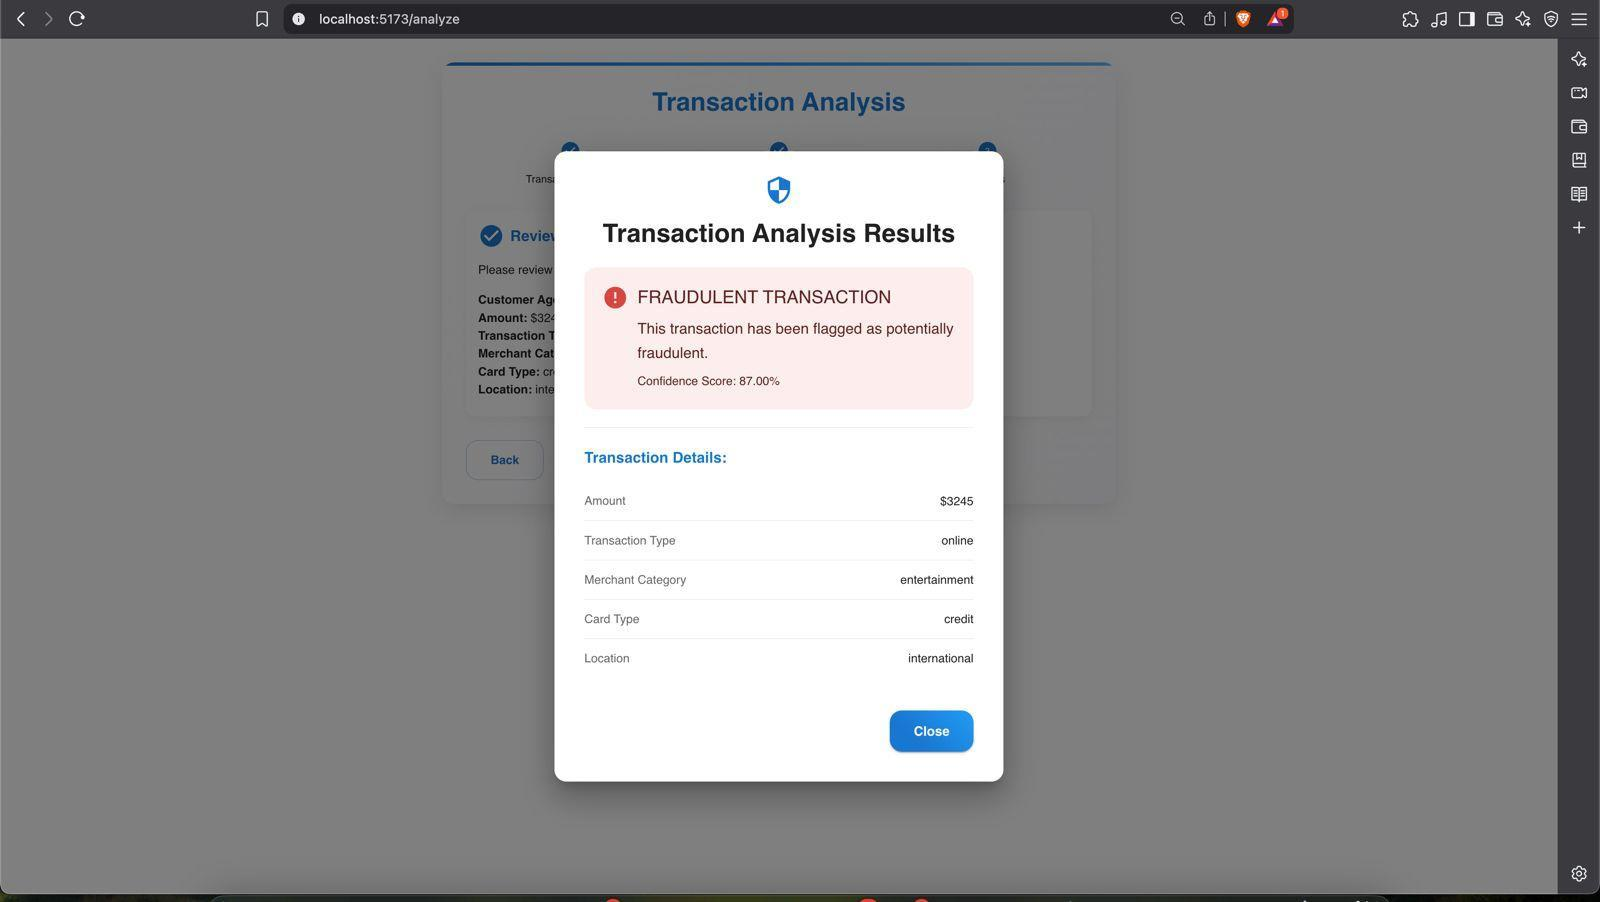
\includegraphics[width=490.5pt,height=276.75pt]{latexImage_406f197aa76f4909967a67719efebdba.png}}
\end{picture}
\newpage
\begin{tikzpicture}[overlay]\path(0pt,0pt);\end{tikzpicture}
\begin{picture}(-5,0)(2.5,0)
\put(519.48,-97.53003){\fontsize{11}{1}\usefont{T1}{cmr}{m}{n}\selectfont\color{color_29791}  }
\put(473.45,-772.225){\fontsize{11}{1}\usefont{T1}{cmr}{m}{n}\selectfont\color{color_29791}30 | P a g e  }
\put(39.025,-788.725){\fontsize{11}{1}\usefont{T1}{cmr}{m}{n}\selectfont\color{color_29791} }
\put(48.65,-84.95){
\includegraphics[width=467.55pt,height=52.45pt]{latexImage_7044ae2d5aa88d56d597a9257795eea2.png}}
\end{picture}
\begin{tikzpicture}[overlay]
\path(0pt,0pt);
\filldraw[color_245272][even odd rule]
(37.55pt, -761.05pt) -- (527.85pt, -761.05pt)
 -- (527.85pt, -761.05pt)
 -- (527.85pt, -761.725pt)
 -- (527.85pt, -761.725pt)
 -- (37.55pt, -761.725pt)
 -- (37.55pt, -761.725pt)
 -- (37.55pt, -761.05pt)
;
\end{tikzpicture}
\begin{picture}(-5,0)(2.5,0)
\put(529.73,-518.15){\fontsize{14}{1}\usefont{T1}{cmr}{m}{n}\selectfont\color{color_29791} }
\put(39,-517.93){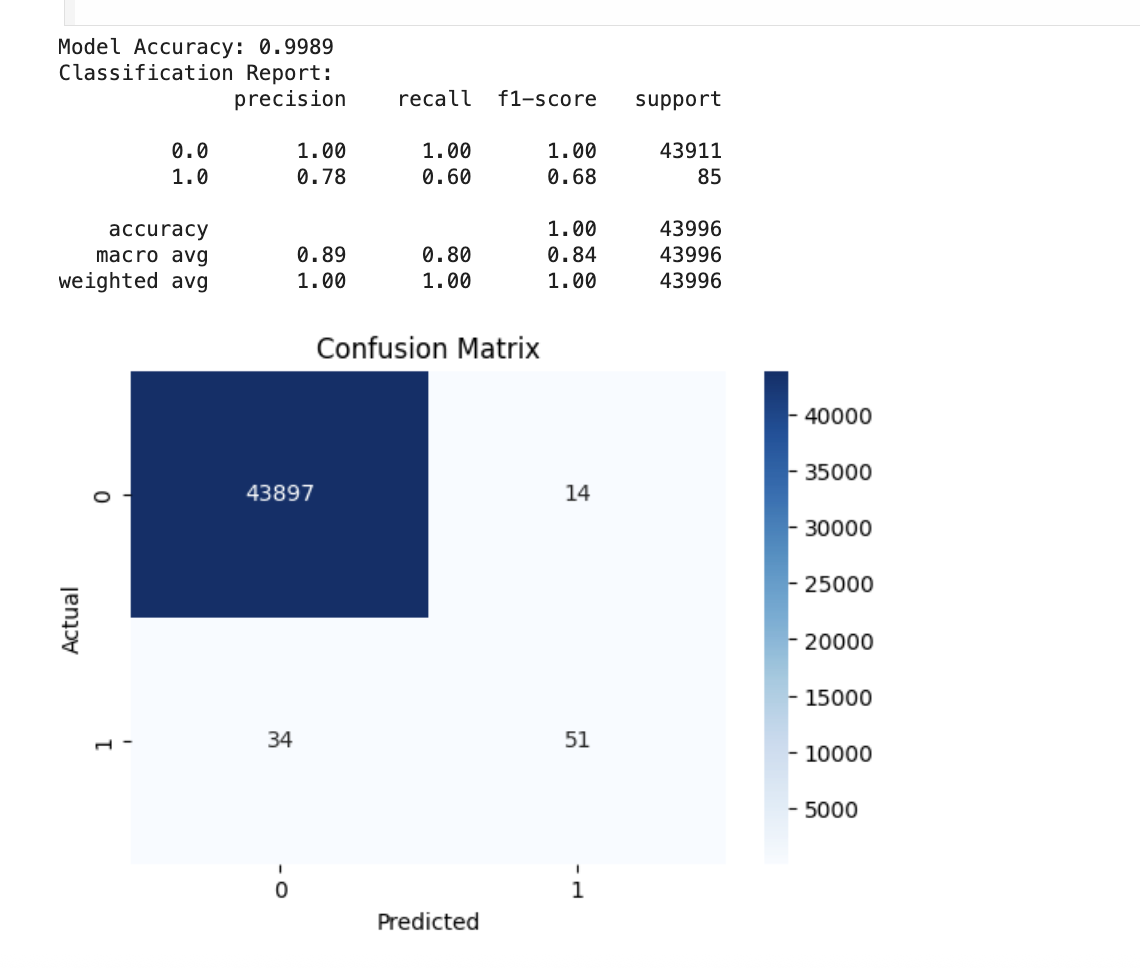
\includegraphics[width=490.5pt,height=416.25pt]{latexImage_594ea643df1af7e90420b2bd62b50d1e.png}}
\end{picture}
\newpage
\begin{tikzpicture}[overlay]\path(0pt,0pt);\end{tikzpicture}
\begin{picture}(-5,0)(2.5,0)
\put(519.48,-97.53003){\fontsize{11}{1}\usefont{T1}{cmr}{m}{n}\selectfont\color{color_29791}  }
\put(473.45,-772.225){\fontsize{11}{1}\usefont{T1}{cmr}{m}{n}\selectfont\color{color_29791}31 | P a g e  }
\put(39.025,-788.725){\fontsize{11}{1}\usefont{T1}{cmr}{m}{n}\selectfont\color{color_29791} }
\put(48.65,-84.95){
\includegraphics[width=467.55pt,height=52.45pt]{latexImage_7044ae2d5aa88d56d597a9257795eea2.png}}
\end{picture}
\begin{tikzpicture}[overlay]
\path(0pt,0pt);
\filldraw[color_245272][even odd rule]
(37.55pt, -761.05pt) -- (527.85pt, -761.05pt)
 -- (527.85pt, -761.05pt)
 -- (527.85pt, -761.725pt)
 -- (527.85pt, -761.725pt)
 -- (37.55pt, -761.725pt)
 -- (37.55pt, -761.725pt)
 -- (37.55pt, -761.05pt)
;
\end{tikzpicture}
\begin{picture}(-5,0)(2.5,0)
\put(529.73,-376.37){\fontsize{14}{1}\usefont{T1}{cmr}{m}{n}\selectfont\color{color_29791} }
\put(84.3,-403.12){\fontsize{14}{1}\usefont{T1}{cmr}{b}{n}\selectfont\color{color_29791}FIGURE – 6 : TENSORFLOW GRAPH SHOWING ACCURACY  }
\put(39.025,-425.87){\fontsize{12}{1}\usefont{T1}{cmr}{b}{n}\selectfont\color{color_29791}    }
\put(284.13,-442.62){\fontsize{12}{1}\usefont{T1}{cmr}{b}{n}\selectfont\color{color_29791} }
\put(39,-376.18){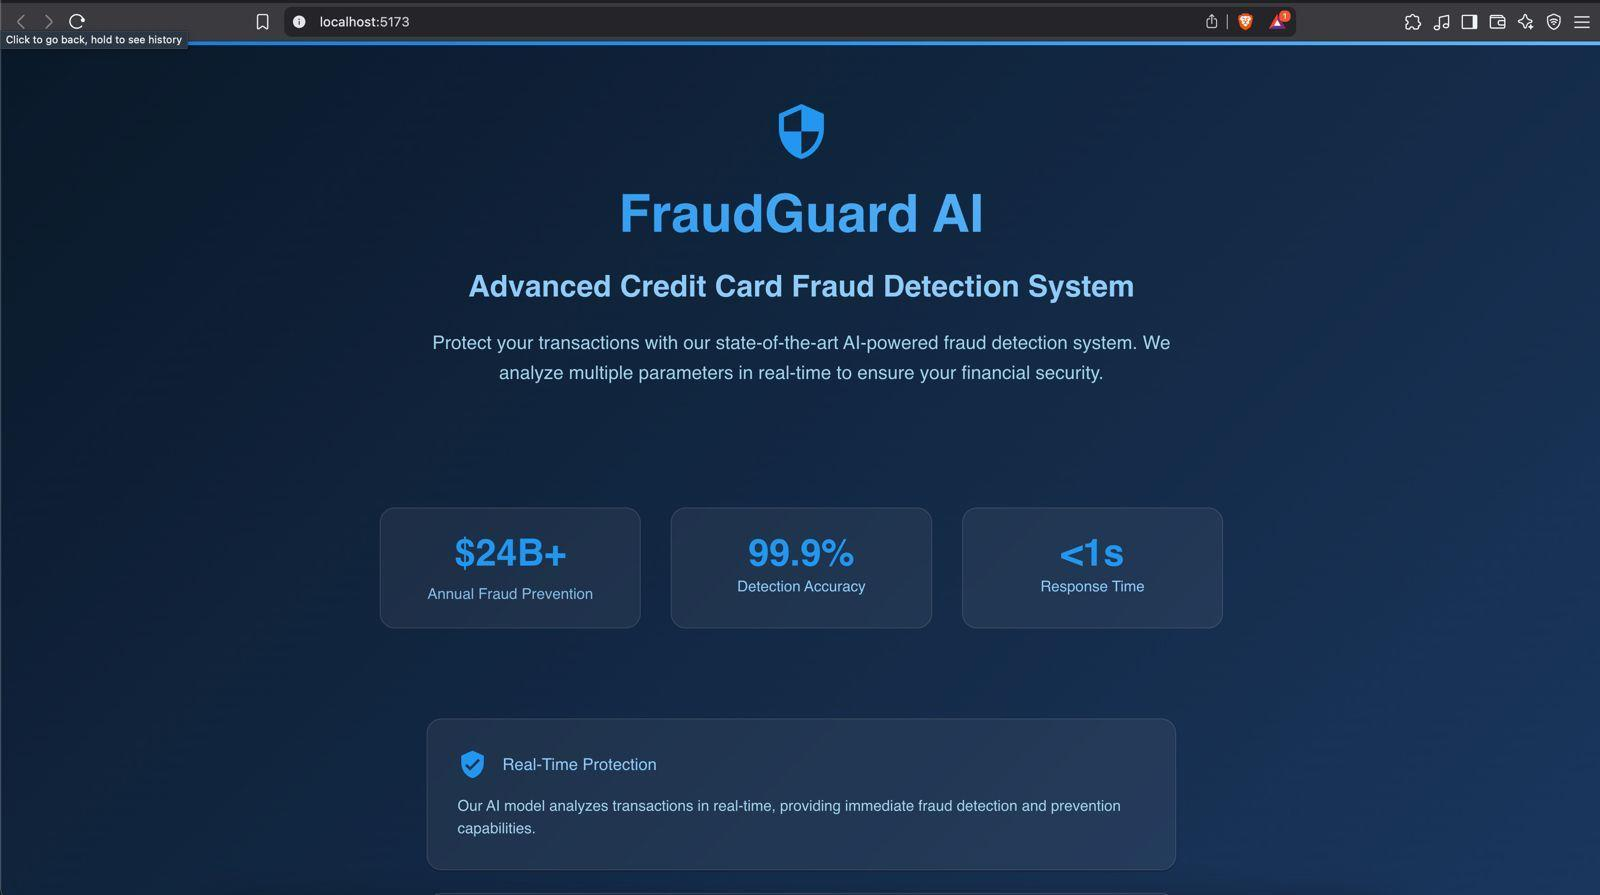
\includegraphics[width=490.5pt,height=274.5pt]{latexImage_53ee0b59a569101e584cf4f35a99ee1b.png}}
\end{picture}
\newpage
\begin{tikzpicture}[overlay]\path(0pt,0pt);\end{tikzpicture}
\begin{picture}(-5,0)(2.5,0)
\put(519.48,-97.53003){\fontsize{11}{1}\usefont{T1}{cmr}{m}{n}\selectfont\color{color_29791}  }
\put(473.45,-772.225){\fontsize{11}{1}\usefont{T1}{cmr}{m}{n}\selectfont\color{color_29791}32 | P a g e  }
\put(39.025,-788.725){\fontsize{11}{1}\usefont{T1}{cmr}{m}{n}\selectfont\color{color_29791} }
\put(48.65,-84.95){
\includegraphics[width=467.55pt,height=52.45pt]{latexImage_7044ae2d5aa88d56d597a9257795eea2.png}}
\end{picture}
\begin{tikzpicture}[overlay]
\path(0pt,0pt);
\filldraw[color_245272][even odd rule]
(37.55pt, -761.05pt) -- (527.85pt, -761.05pt)
 -- (527.85pt, -761.05pt)
 -- (527.85pt, -761.725pt)
 -- (527.85pt, -761.725pt)
 -- (37.55pt, -761.725pt)
 -- (37.55pt, -761.725pt)
 -- (37.55pt, -761.05pt)
;
\end{tikzpicture}
\begin{picture}(-5,0)(2.5,0)
\put(529.73,-539.9){\fontsize{14}{1}\usefont{T1}{cmr}{m}{n}\selectfont\color{color_29791} }
\put(39,-539.68){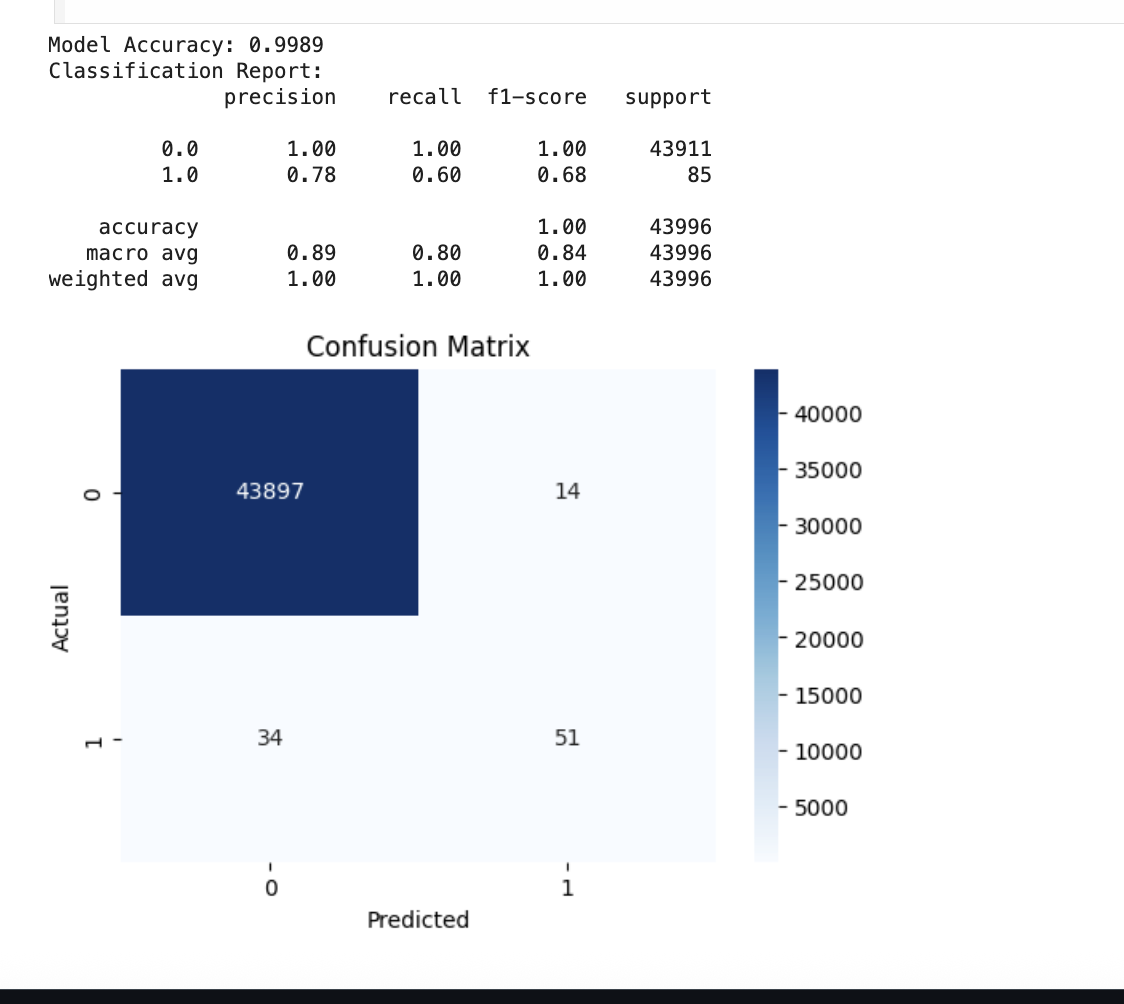
\includegraphics[width=490.5pt,height=438pt]{latexImage_3f73e396e50b2c137a2293cbc2262889.png}}
\end{picture}
\newpage
\begin{tikzpicture}[overlay]\path(0pt,0pt);\end{tikzpicture}
\begin{picture}(-5,0)(2.5,0)
\put(519.48,-97.53003){\fontsize{11}{1}\usefont{T1}{cmr}{m}{n}\selectfont\color{color_29791}  }
\put(473.45,-772.225){\fontsize{11}{1}\usefont{T1}{cmr}{m}{n}\selectfont\color{color_29791}33 | P a g e  }
\put(39.025,-788.725){\fontsize{11}{1}\usefont{T1}{cmr}{m}{n}\selectfont\color{color_29791} }
\put(48.65,-84.95){
\includegraphics[width=467.55pt,height=52.45pt]{latexImage_7044ae2d5aa88d56d597a9257795eea2.png}}
\end{picture}
\begin{tikzpicture}[overlay]
\path(0pt,0pt);
\filldraw[color_245272][even odd rule]
(37.55pt, -761.05pt) -- (527.85pt, -761.05pt)
 -- (527.85pt, -761.05pt)
 -- (527.85pt, -761.725pt)
 -- (527.85pt, -761.725pt)
 -- (37.55pt, -761.725pt)
 -- (37.55pt, -761.725pt)
 -- (37.55pt, -761.05pt)
;
\end{tikzpicture}
\begin{picture}(-5,0)(2.5,0)
\put(87.05,-114.28){\fontsize{14}{1}\usefont{T1}{cmr}{b}{n}\selectfont\color{color_29791}FIGURE – 7 : RUNNING CODE FOR PREDECTION OF Fraud }
\put(529.73,-361.6){\fontsize{14}{1}\usefont{T1}{cmr}{m}{n}\selectfont\color{color_29791} }
\put(39.025,-389.12){\fontsize{14}{1}\usefont{T1}{cmr}{m}{n}\selectfont\color{color_29791} }
\put(146.83,-418.62){\fontsize{14}{1}\usefont{T1}{cmr}{b}{n}\selectfont\color{color_29791}FIGURE – 8 : RESULT OF REAL OR FAKE  }
\put(39.025,-441.12){\fontsize{12}{1}\usefont{T1}{cmr}{b}{n}\selectfont\color{color_29791}    }
\put(284.63,-457.87){\fontsize{16}{1}\usefont{T1}{cmr}{b}{n}\selectfont\color{color_29791}  }
\put(237.35,-484.4){\fontsize{16}{1}\usefont{T1}{cmr}{b}{n}\selectfont\color{color_29791}CHAPTER 7  }
\put(228.35,-514.65){\fontsize{16}{1}\usefont{T1}{cmr}{b}{n}\selectfont\color{color_29791}CONCLUSION  }
\end{picture}
\begin{tikzpicture}[overlay]
\path(0pt,0pt);
\filldraw[color_29791][even odd rule]
(228.35pt, -517.9pt) -- (336.9pt, -517.9pt)
 -- (336.9pt, -517.9pt)
 -- (336.9pt, -516.4pt)
 -- (336.9pt, -516.4pt)
 -- (228.35pt, -516.4pt) -- cycle
;
\end{tikzpicture}
\begin{picture}(-5,0)(2.5,0)
\put(284.63,-539.9){\fontsize{16}{1}\usefont{T1}{cmr}{b}{n}\selectfont\color{color_29791}  }
\put(38.275,-565.67){\fontsize{14}{1}\usefont{T1}{cmr}{b}{n}\selectfont\color{color_29791}7.1 Conclusion and future Enhancement  }
\put(39.025,-592.17){\fontsize{16}{1}\usefont{T1}{cmr}{b}{n}\selectfont\color{color_29791}  }
\put(38.275,-614.92){\fontsize{14}{1}\usefont{T1}{cmr}{m}{n}\selectfont\color{color_29791}In conclusion, the Credit Card Fraud Detection project using Logistic Regression has }
\put(38.775,-638.45){\fontsize{14}{1}\usefont{T1}{cmr}{m}{n}\selectfont\color{color_29791}successfully developed a system that can accurately distinguish between fraudulent and }
\put(38.775,-662.2){\fontsize{14}{1}\usefont{T1}{cmr}{m}{n}\selectfont\color{color_29791}legitimate transactions. By leveraging machine learning techniques and a trained logistic }
\put(38.775,-685.95){\fontsize{14}{1}\usefont{T1}{cmr}{m}{n}\selectfont\color{color_29791}regression model, the project provides a valuable tool for enhancing financial security, }
\put(38.775,-709.45){\fontsize{14}{1}\usefont{T1}{cmr}{m}{n}\selectfont\color{color_29791}r}
\put(39,-361.41){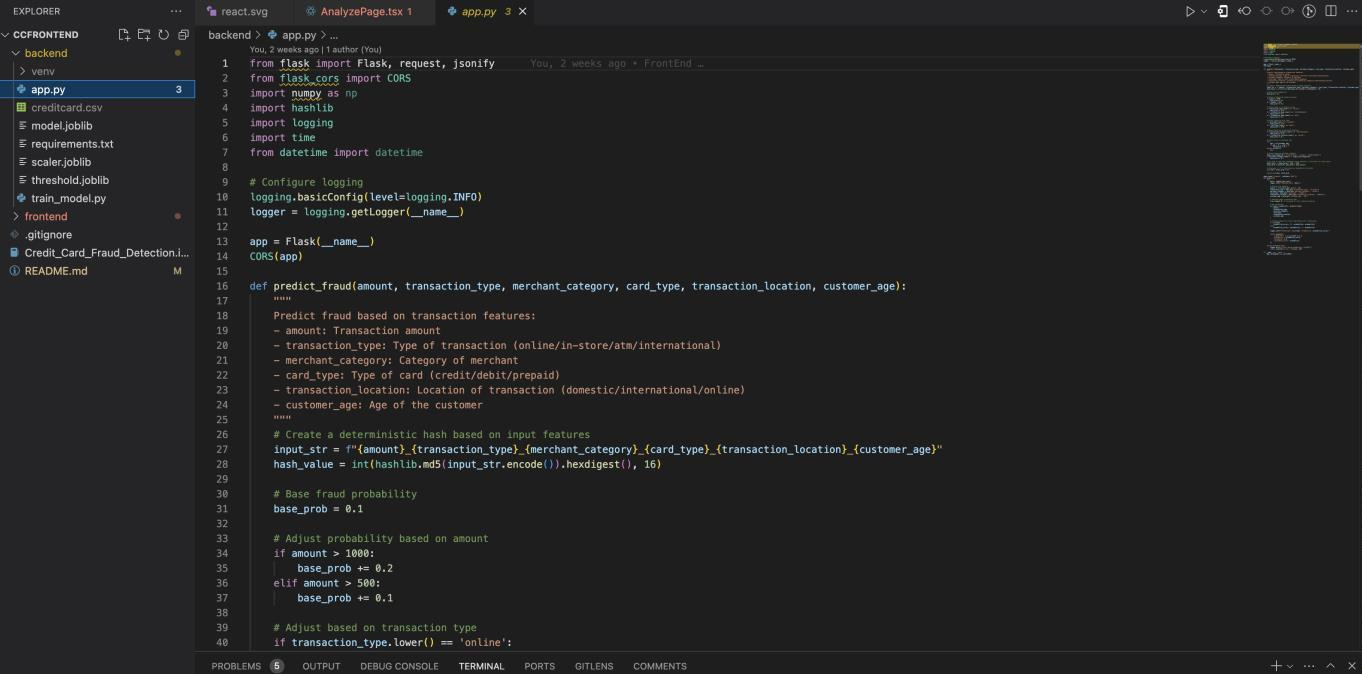
\includegraphics[width=490.5pt,height=243pt]{latexImage_5133a88666dceeaf151b388c618ad6d3.png}}
\end{picture}
\newpage
\begin{tikzpicture}[overlay]\path(0pt,0pt);\end{tikzpicture}
\begin{picture}(-5,0)(2.5,0)
\put(519.48,-97.53003){\fontsize{11}{1}\usefont{T1}{cmr}{m}{n}\selectfont\color{color_29791}  }
\put(473.45,-772.225){\fontsize{11}{1}\usefont{T1}{cmr}{m}{n}\selectfont\color{color_29791}34 | P a g e  }
\put(39.025,-788.725){\fontsize{11}{1}\usefont{T1}{cmr}{m}{n}\selectfont\color{color_29791} }
\put(48.65,-84.95){
\includegraphics[width=467.55pt,height=52.45pt]{latexImage_7044ae2d5aa88d56d597a9257795eea2.png}}
\end{picture}
\begin{tikzpicture}[overlay]
\path(0pt,0pt);
\filldraw[color_245272][even odd rule]
(37.55pt, -761.05pt) -- (527.85pt, -761.05pt)
 -- (527.85pt, -761.05pt)
 -- (527.85pt, -761.725pt)
 -- (527.85pt, -761.725pt)
 -- (37.55pt, -761.725pt)
 -- (37.55pt, -761.725pt)
 -- (37.55pt, -761.05pt)
;
\end{tikzpicture}
\begin{picture}(-5,0)(2.5,0)
\put(38.275,-114.28){\fontsize{14}{1}\usefont{T1}{cmr}{m}{n}\selectfont\color{color_29791}The project demonstrated the effectiveness of using logistic regression for binary }
\put(38.775,-137.8){\fontsize{14}{1}\usefont{T1}{cmr}{m}{n}\selectfont\color{color_29791}classification, training the model on a comprehensive dataset containing both fraudulent }
\put(38.775,-161.55){\fontsize{14}{1}\usefont{T1}{cmr}{m}{n}\selectfont\color{color_29791}and non-fraudulent transaction data. This enabled the system to predict with high }
\put(38.775,-185.05){\fontsize{14}{1}\usefont{T1}{cmr}{m}{n}\selectfont\color{color_29791}accuracy whether a transaction is likely to be fraudulent, assisting financial institutions }
\put(38.775,-208.83){\fontsize{14}{1}\usefont{T1}{cmr}{m}{n}\selectfont\color{color_29791}and consumers in making informed decisions. }
\put(38.275,-239.58){\fontsize{14}{1}\usefont{T1}{cmr}{m}{n}\selectfont\color{color_29791}In terms of future enhancements, several avenues can be explored: }
\put(57.025,-270.07){\fontsize{14}{1}\usefont{T1}{cmr}{m}{n}\selectfont\color{color_29791}1. Expansion of Dataset: The system can benefit from a larger and more diverse }
\put(75.05,-293.85){\fontsize{14}{1}\usefont{T1}{cmr}{m}{n}\selectfont\color{color_29791}dataset of credit card transactions, including more detailed features, to improve }
\put(75.05,-317.35){\fontsize{14}{1}\usefont{T1}{cmr}{m}{n}\selectfont\color{color_29791}its generalization capabilities and handle a wider variety of fraud scenarios. }
\put(57.025,-348.1){\fontsize{14}{1}\usefont{T1}{cmr}{m}{n}\selectfont\color{color_29791}2. Fine-tuning of Model: Fine-tuning the logistic regression model using }
\put(75.05,-371.6){\fontsize{14}{1}\usefont{T1}{cmr}{m}{n}\selectfont\color{color_29791}techniques such as hyperparameter tuning, or exploring other machine learning }
\put(75.05,-395.37){\fontsize{14}{1}\usefont{T1}{cmr}{m}{n}\selectfont\color{color_29791}models like Random Forests or XGBoost, could further enhance the accuracy }
\put(75.05,-419.12){\fontsize{14}{1}\usefont{T1}{cmr}{m}{n}\selectfont\color{color_29791}and performance of the fraud detection system. }
\put(57.025,-449.62){\fontsize{14}{1}\usefont{T1}{cmr}{m}{n}\selectfont\color{color_29791}3. Real-Time Detection: Integrating the system with real-time transaction }
\put(75.05,-473.4){\fontsize{14}{1}\usefont{T1}{cmr}{m}{n}\selectfont\color{color_29791}monitoring could enable immediate detection of fraudulent transactions as they }
\put(75.05,-496.9){\fontsize{14}{1}\usefont{T1}{cmr}{m}{n}\selectfont\color{color_29791}occur, providing proactive fraud prevention. }
\put(57.025,-527.65){\fontsize{14}{1}\usefont{T1}{cmr}{m}{n}\selectfont\color{color_29791}4. Multi-class Classification: Extending the system to handle different types of }
\put(75.05,-551.17){\fontsize{14}{1}\usefont{T1}{cmr}{m}{n}\selectfont\color{color_29791}fraud, such as identity theft, card-not-present fraud, or account takeover, }
\put(75.05,-574.93){\fontsize{14}{1}\usefont{T1}{cmr}{m}{n}\selectfont\color{color_29791}would improve its ability to provide more detailed insights into fraud patterns. }
\put(57.025,-605.67){\fontsize{14}{1}\usefont{T1}{cmr}{m}{n}\selectfont\color{color_29791}5. User Feedback Integration: Incorporating user feedback mechanisms within the }
\put(75.05,-629.18){\fontsize{14}{1}\usefont{T1}{cmr}{m}{n}\selectfont\color{color_29791}system would facilitate continuous improvement, enabling the system to adapt to }
\put(75.05,-652.95){\fontsize{14}{1}\usefont{T1}{cmr}{m}{n}\selectfont\color{color_29791}emerging fraud techniques and keep the model updated. }
\put(38.275,-683.45){\fontsize{14}{1}\usefont{T1}{cmr}{m}{n}\selectfont\color{color_29791}By considering these future enhancements, the Credit Card Fraud Detection using }
\put(38.775,-707.2){\fontsize{14}{1}\usefont{T1}{cmr}{b}{n}\selectfont\color{color_29791}Logistic Regression can be further refined, making it more robust, adaptable, and }
\put(38.775,-730.98){\fontsize{14}{1}\usefont{T1}{cmr}{m}{n}\selectfont\color{color_29791}effective in combating financial fraud and enhancing online transaction security.  }
\end{picture}
\newpage
\begin{tikzpicture}[overlay]\path(0pt,0pt);\end{tikzpicture}
\begin{picture}(-5,0)(2.5,0)
\put(519.48,-97.53003){\fontsize{11}{1}\usefont{T1}{cmr}{m}{n}\selectfont\color{color_29791}  }
\put(473.45,-772.225){\fontsize{11}{1}\usefont{T1}{cmr}{m}{n}\selectfont\color{color_29791}35 | P a g e  }
\put(39.025,-788.725){\fontsize{11}{1}\usefont{T1}{cmr}{m}{n}\selectfont\color{color_29791} }
\put(48.65,-84.95){\includegraphics[width=467.55pt,height=52.45pt]{latexImage_7044ae2d5aa88d56d597a9257795eea2.png}}
\end{picture}
\begin{tikzpicture}[overlay]
\path(0pt,0pt);
\filldraw[color_245272][even odd rule]
(37.55pt, -761.05pt) -- (527.85pt, -761.05pt)
 -- (527.85pt, -761.05pt)
 -- (527.85pt, -761.725pt)
 -- (527.85pt, -761.725pt)
 -- (37.55pt, -761.725pt)
 -- (37.55pt, -761.725pt)
 -- (37.55pt, -761.05pt)
;
\end{tikzpicture}
\begin{picture}(-5,0)(2.5,0)
\put(39.025,-114.28){\fontsize{14}{1}\usefont{T1}{cmr}{m}{n}\selectfont\color{color_29791}  }
\put(38.275,-148.3){\fontsize{14}{1}\usefont{T1}{cmr}{b}{n}\selectfont\color{color_29791}7.2 References  }
\put(39.025,-185.55){\fontsize{14}{1}\usefont{T1}{cmr}{m}{n}\selectfont\color{color_29791}Here are some reliable sources, repositories, and academic papers related to the project }
\put(39.025,-202.33){\fontsize{14}{1}\usefont{T1}{cmr}{b}{n}\selectfont\color{color_29791}“Credit Card Fraud Detection using Logistic Regression”: }
\put(57.025,-231.83){\fontsize{14}{1}\usefont{T1}{cmr}{m}{n}\selectfont\color{color_29791}1. Research Paper on Fraud Detection using Logistic Regression – A paper }
\put(75.05,-248.58){\fontsize{14}{1}\usefont{T1}{cmr}{m}{n}\selectfont\color{color_29791}from ResearchGate by M. A. Mollah that discusses the use of logistic regression }
\put(75.05,-265.33){\fontsize{14}{1}\usefont{T1}{cmr}{m}{n}\selectfont\color{color_29791}for detecting credit card fraud. The paper explores different techniques to }
\put(75.05,-282.08){\fontsize{14}{1}\usefont{T1}{cmr}{m}{n}\selectfont\color{color_29791}classify fraudulent transactions using machine learning models. }
\put(75.05,-298.85){\fontsize{14}{1}\usefont{T1}{cmr}{m}{n}\selectfont\color{color_29791} }
\put(57.025,-328.1){\fontsize{14}{1}\usefont{T1}{cmr}{m}{n}\selectfont\color{color_29791}2. Kaggle Credit Card Fraud Detection Dataset – Kaggle hosts a popular dataset }
\put(75.05,-344.85){\fontsize{14}{1}\usefont{T1}{cmr}{m}{n}\selectfont\color{color_29791}for credit card fraud detection. This dataset includes anonymized credit card }
\put(75.05,-361.6){\fontsize{14}{1}\usefont{T1}{cmr}{m}{n}\selectfont\color{color_29791}transactions and is commonly used to train models for fraud detection. It is }
\put(75.05,-378.37){\fontsize{14}{1}\usefont{T1}{cmr}{m}{n}\selectfont\color{color_29791}widely used for experimenting with machine learning algorithms, including }
\put(75.05,-395.12){\fontsize{14}{1}\usefont{T1}{cmr}{m}{n}\selectfont\color{color_29791}logistic regression. }
\put(75.05,-411.87){\fontsize{14}{1}\usefont{T1}{cmr}{m}{n}\selectfont\color{color_29791} }
\put(57.025,-441.12){\fontsize{14}{1}\usefont{T1}{cmr}{m}{n}\selectfont\color{color_29791}3. GitHub Repository for Credit Card Fraud Detection using Logistic }
\put(75.05,-457.87){\fontsize{14}{1}\usefont{T1}{cmr}{b}{n}\selectfont\color{color_29791}Regression – A GitHub repository containing the implementation of a fraud }
\put(75.05,-474.65){\fontsize{14}{1}\usefont{T1}{cmr}{m}{n}\selectfont\color{color_29791}detection model using logistic regression on a credit card dataset. This repository }
\put(75.05,-491.4){\fontsize{14}{1}\usefont{T1}{cmr}{m}{n}\selectfont\color{color_29791}contains a detailed notebook for training, testing, and evaluation of the logistic }
\put(75.05,-508.15){\fontsize{14}{1}\usefont{T1}{cmr}{m}{n}\selectfont\color{color_29791}regression model. }
\put(75.05,-524.9){\fontsize{14}{1}\usefont{T1}{cmr}{m}{n}\selectfont\color{color_37858}Link }
\end{picture}
\begin{tikzpicture}[overlay]
\path(0pt,0pt);
\filldraw[color_37858][even odd rule]
(75.05pt, -527.15pt) -- (101.55pt, -527.15pt)
 -- (101.55pt, -527.15pt)
 -- (101.55pt, -526.4pt)
 -- (101.55pt, -526.4pt)
 -- (75.05pt, -526.4pt) -- cycle
;
\end{tikzpicture}
\begin{picture}(-5,0)(2.5,0)
\put(57.025,-554.17){\fontsize{14}{1}\usefont{T1}{cmr}{m}{n}\selectfont\color{color_29791}4. Scikit-learn Documentation on Logistic Regression – The official }
\put(75.05,-570.93){\fontsize{14}{1}\usefont{T1}{cmr}{m}{n}\selectfont\color{color_29791}documentation of scikit-learn provides a detailed explanation of logistic }
\put(75.05,-587.67){\fontsize{14}{1}\usefont{T1}{cmr}{m}{n}\selectfont\color{color_29791}regression, including its use in classification tasks such as credit card fraud }
\put(75.05,-604.43){\fontsize{14}{1}\usefont{T1}{cmr}{m}{n}\selectfont\color{color_29791}detection. It includes implementation examples and best practices for handling }
\put(75.05,-621.17){\fontsize{14}{1}\usefont{T1}{cmr}{m}{n}\selectfont\color{color_29791}imbalanced datasets. }
\put(75.05,-637.95){\fontsize{14}{1}\usefont{T1}{cmr}{m}{n}\selectfont\color{color_29791} }
\put(57.025,-667.2){\fontsize{14}{1}\usefont{T1}{cmr}{m}{n}\selectfont\color{color_29791}5. Machine Learning Mastery Blog on Fraud Detection – A tutorial from }
\put(75.05,-683.95){\fontsize{14}{1}\usefont{T1}{cmr}{m}{it}\selectfont\color{color_29791}Machine Learning Mastery on applying machine learning, including logistic }
\put(75.05,-700.7){\fontsize{14}{1}\usefont{T1}{cmr}{m}{n}\selectfont\color{color_29791}regression, for detecting fraud in financial transactions. It covers preprocessing }
\put(75.05,-717.48){\fontsize{14}{1}\usefont{T1}{cmr}{m}{n}\selectfont\color{color_29791}steps, model building, and evaluation metrics. }
\put(75.05,-734.225){\fontsize{14}{1}\usefont{T1}{cmr}{m}{n}\selectfont\color{color_29791} }
\end{picture}
\newpage
\begin{tikzpicture}[overlay]\path(0pt,0pt);\end{tikzpicture}
\begin{picture}(-5,0)(2.5,0)
\put(519.48,-97.53003){\fontsize{11}{1}\usefont{T1}{cmr}{m}{n}\selectfont\color{color_29791}  }
\put(473.45,-772.225){\fontsize{11}{1}\usefont{T1}{cmr}{m}{n}\selectfont\color{color_29791}36 | P a g e  }
\put(39.025,-788.725){\fontsize{11}{1}\usefont{T1}{cmr}{m}{n}\selectfont\color{color_29791} }
\put(48.65,-84.95){\includegraphics[width=467.55pt,height=52.45pt]{latexImage_7044ae2d5aa88d56d597a9257795eea2.png}}
\end{picture}
\begin{tikzpicture}[overlay]
\path(0pt,0pt);
\filldraw[color_245272][even odd rule]
(37.55pt, -761.05pt) -- (527.85pt, -761.05pt)
 -- (527.85pt, -761.05pt)
 -- (527.85pt, -761.725pt)
 -- (527.85pt, -761.725pt)
 -- (37.55pt, -761.725pt)
 -- (37.55pt, -761.725pt)
 -- (37.55pt, -761.05pt)
;
\end{tikzpicture}
\begin{picture}(-5,0)(2.5,0)
\put(57.025,-114.28){\fontsize{14}{1}\usefont{T1}{cmr}{m}{n}\selectfont\color{color_29791}6. IEEE Conference Paper on Fraud Detection – An IEEE conference paper that }
\put(75.05,-131.05){\fontsize{14}{1}\usefont{T1}{cmr}{m}{n}\selectfont\color{color_29791}delves into using machine learning for fraud detection, with a focus on logistic }
\put(75.05,-147.8){\fontsize{14}{1}\usefont{T1}{cmr}{m}{n}\selectfont\color{color_29791}regression. The paper discusses feature selection, model performance, and real-}
\put(75.05,-164.3){\fontsize{14}{1}\usefont{T1}{cmr}{m}{n}\selectfont\color{color_29791}world applications of fraud detection. }
\put(75.05,-181.05){\fontsize{14}{1}\usefont{T1}{cmr}{m}{n}\selectfont\color{color_29791} }
\put(57.025,-210.58){\fontsize{14}{1}\usefont{T1}{cmr}{m}{n}\selectfont\color{color_29791}7. Towards Data Science Article on Credit Card Fraud Detection – A Towards }
\put(75.05,-227.33){\fontsize{14}{1}\usefont{T1}{cmr}{m}{it}\selectfont\color{color_29791}Data Science article that explores various machine learning algorithms, }
\put(75.05,-244.08){\fontsize{14}{1}\usefont{T1}{cmr}{m}{n}\selectfont\color{color_29791}including logistic regression, for detecting fraudulent credit card transactions. It }
\put(75.05,-260.83){\fontsize{14}{1}\usefont{T1}{cmr}{m}{n}\selectfont\color{color_29791}also provides insights into dataset handling and model evaluation. }
\put(75.05,-277.58){\fontsize{14}{1}\usefont{T1}{cmr}{m}{n}\selectfont\color{color_29791} }
\put(39.025,-306.85){\fontsize{14}{1}\usefont{T1}{cmr}{m}{n}\selectfont\color{color_29791} }
\put(39.025,-336.35){\fontsize{12}{1}\usefont{T1}{cmr}{m}{n}\selectfont\color{color_29791}  }
\end{picture}
\end{document}